\documentclass[url, 11pt, fleqn, openany, chapterprefix=off]{scrbook}
%\documentclass[url, 11pt, fleqn, openany, chapterprefix=off]{book}
%\documentclass[url,11pt,fleqn]{book} % Default font size and left-justified equations
%\documentclass[url,11pt,fleqn]{article} % Default font size and left-justified equations
%\addtokomafont{disposition}{\rmfamily}
%%% colors for quick comments
\newcommand{\tcr}{\textcolor{red}}
\newcommand{\tcb}{\textcolor{blue}}
\newcommand{\tcm}{\textcolor{magenta}}
\newcommand{\tcg}{\textcolor{green}}
\newcommand{\tcp}{\textcolor{purple}}

\usepackage[pagestyles]{titlesec}


%----------------------------------------------------------------------------------------
%	VARIOUS REQUIRED PACKAGES
%----------------------------------------------------------------------------------------
%\usepackage[top=3cm,bottom=3cm,left=3.2cm,right=3.2cm,headsep=30pt]{geometry} % Page margins
\usepackage[top=3cm,bottom=3cm,left=2.5cm,right=2.5cm,headsep=10pt,a4paper]{geometry} % Page margins
\usepackage{xcolor} % Required for specifying colors by name
\definecolor{ocre}{RGB}{52,177,201} % Define the orange color used for highlighting throughout the book

\usepackage[colorinlistoftodos,prependcaption,textsize=tiny]{todonotes}


% Font Settings
\usepackage{avant} % Use the Avantgarde font for headings
%\usepackage{times} % Use the Times font for headings
\usepackage{mathptmx} % Use the Adobe Times Roman as the default text font together with math symbols from the Sym­bol, Chancery and Computer Modern fonts

\usepackage{microtype} % Slightly tweak font spacing for aesthetics
\usepackage[utf8]{inputenc} % Required for including letters with accents
\usepackage[T1]{fontenc} % Use 8-bit encoding that has 256 glyphs

% Bibliography
%\usepackage[style=alphabetic,sorting=nyt,sortcites=true,autopunct=true,babel=hyphen,hyperref=true,abbreviate=false,backref=true,backend=biber]{biblatex}
%\addbibresource{bibliography.bib} % BibTeX bibliography file
%\defbibheading{bibempty}{}

\usepackage{placeins} % allows floatbarriers
%\usepackage{titlesec} % Allows customization of titles
%\titleformat{\chapter} % command
%[display] % shape
%{\bfseries\huge} % format
%{Chapter \ \thechapter} % label
%{-2.7ex} % sep
%{\vspace{0ex} \centering} % before-code
%[] % after-code

\usepackage{parskip}
\setlength{\parskip}{.2\baselineskip plus 0pt}

\usepackage{subcaption} %enables subfigures

\usepackage{graphicx} % Required for including pictures
\graphicspath{{Pictures/}{figures/cosmo/}} % Specifies the directory where pictures are stored
\usepackage{wrapfig}
\usepackage{textcomp}
\usepackage{lipsum} % Inserts dummy text

\usepackage{tikz} % Required for drawing custom shapes

\usepackage[english]{babel} % English language/hyphenation

\usepackage{enumitem} % Customize lists
\setlist{nolistsep} % Reduce spacing between bullet points and numbered lists

\usepackage{booktabs} % Required for nicer horizontal rules in tables

\usepackage{eso-pic} % Required for specifying an image background in the title page

%----------------------------------------------------------------------------------------
%	MAIN TABLE OF CONTENTS
%----------------------------------------------------------------------------------------

\usepackage{titletoc} % Required for manipulating the table of contents

\contentsmargin{0cm} % Removes the default margin
% % Chapter text styling
% \titlecontents{chapter}[1.25cm] % Indentation
% {\addvspace{15pt}\large\sffamily\bfseries} % Spacing and font options for chapters
% {\color{ocre!60}\contentslabel[\Large\thecontentslabel]{1.25cm}\color{ocre}} % Chapter number
% {}
% {\color{ocre!60}\normalsize\sffamily\bfseries\;\titlerule*[.5pc]{.}\;\thecontentspage} % Page number

% Section text styling
\titlecontents{section}[1.25cm] % Indentation
{\addvspace{5pt}\sffamily\bfseries} % Spacing and font options for sections
{\contentslabel[\thecontentslabel]{1.25cm}} % Section number
{}
{\sffamily\hfill\color{black}\thecontentspage} % Page number
[]
% Subsection text styling
\titlecontents{subsection}[1.25cm] % Indentation
{\addvspace{1pt}\sffamily\small} % Spacing and font options for subsections
{\contentslabel[\thecontentslabel]{1.25cm}} % Subsection number
{}
{\sffamily\;\titlerule*[.5pc]{.}\;\thecontentspage} % Page number
[]





%----------------------------------------------------------------------------------------
%	PAGE HEADERS
%----------------------------------------------------------------------------------------



\usepackage{fancyhdr} % Required for header and footer configuration

\pagestyle{fancy}
%\renewcommand{\chaptermark}[1]{\markboth{\sffamily\normalsize\bfseries\chaptername\ \thechapter.\ #1}{}} % Chapter text font settings
\renewcommand{\sectionmark}[1]{\markright{\sffamily\normalsize\thesection\hspace{5pt}#1}{}} % Section text font settings
\fancyhf{} \fancyhead[LE,RO]{\sffamily\normalsize\thepage} % Font setting for the page number in the header
\fancyhead[LO]{\rightmark} % Print the nearest section name on the left side of odd pages
\fancyhead[RE]{\leftmark} % Print the current chapter name on the right side of even pages
\renewcommand{\headrulewidth}{0.5pt} % Width of the rule under the header
%\addtolength{\headheight}{26pt} % Increase the spacing around the header slightly
\renewcommand{\footrulewidth}{0pt} % Removes the rule in the footer
\fancypagestyle{plain}{\fancyhead{}\renewcommand{\headrulewidth}{0pt}} % Style for when a plain pagestyle is specified

% Removes the header from odd empty pages at the end of chapters
\makeatletter
\renewcommand{\cleardoublepage}{
\clearpage\ifodd\c@page\else
\hbox{}
\vspace*{\fill}
\thispagestyle{empty}
\newpage
\fi}

%----------------------------------------------------------------------------------------
%	SECTION NUMBERING IN THE MARGIN
%----------------------------------------------------------------------------------------

\makeatletter
\renewcommand{\@seccntformat}[1]{\llap{\textcolor{ocre}{\csname the#1\endcsname}\hspace{1em}}}
\renewcommand{\section}{\@startsection{section}{1}{\z@}
{-4ex \@plus -1ex \@minus -.4ex}
{1ex \@plus.2ex }
{\normalfont\large\sffamily\bfseries}}
\renewcommand{\subsection}{\@startsection {subsection}{2}{\z@}
{-3ex \@plus -0.1ex \@minus -.4ex}
{0.5ex \@plus.2ex }
{\normalfont\sffamily\bfseries}}
\renewcommand{\subsubsection}{\@startsection {subsubsection}{3}{\z@}
{-2ex \@plus -0.1ex \@minus -.2ex}
{.2ex \@plus.2ex }
{\normalfont\small\sffamily\bfseries}}
\renewcommand\paragraph{\@startsection{paragraph}{4}{\z@}
{-2ex \@plus-.2ex \@minus .2ex}
{.1ex}
{\normalfont\small\sffamily\bfseries}}

%----------------------------------------------------------------------------------------
%	HYPERLINKS IN THE DOCUMENTS
%----------------------------------------------------------------------------------------

% For an unclear reason, the package should be loaded now and not later
\usepackage{hyperref}
%\hypersetup{hidelinks,backref=true,pagebackref=true,hyperindex=true,colorlinks=false,breaklinks=true,urlcolor= ocre,bookmarks=true,bookmarksopen=false,pdftitle={Title},pdfauthor={Author}}
 \hypersetup{hidelinks,
            %backref=true,
            %pagebackref=true,
            %hyperindex=true,
            breaklinks=true,
            %bookmarks=true,
            bookmarksopen=false,
            pdftitle={Title},
            pdfauthor={Author}
            colorlinks=true,
            pdfstartview=FitV,
            linkcolor=Blue,
            citecolor=MediumBlue,
            urlcolor=IndianRed}

%needed for cosmo
\usepackage{graphicx}
\graphicspath{{./figures/}}
%\usepackage{psfrag}
\usepackage{appendix}
\usepackage{latexsym,amsmath,amsfonts,amssymb,booktabs}
\usepackage[font=small]{caption}
\usepackage{slashed,upgreek,amscd,cancel,tensor,color}
\usepackage{adjustbox}
\usepackage[numbers,compress,square]{natbib}
\usepackage{epsfig,latexsym}
%\usepackage[pdfencoding=auto]{hyperref}
\usepackage{url}
\numberwithin{equation}{section}% numera le equazioni seconde le sezioni , e.g. 1.15 invece che consecutivamente; anche le appendici, eq. (A.1) etc. Richiede amsmath
\usepackage{doi}
\usepackage{subcaption}
\usepackage{mathtools}
\usepackage{upgreek}
\usepackage{stfloats}
\usepackage{afterpage}
\usepackage{multirow}

%\usepackage{hyperref}
%\usepackage[usenames,table,dvipsnames,svgnames]{xcolor}
\usepackage{pdfpages}
\usepackage[squaren]{SIunits}
\usepackage{acronym}
\usepackage{tcolorbox}
%\usepackage{etoolbox}
\usepackage{multicol}
 \usepackage{vwcol}
\usepackage{placeins}
\usepackage[absolute]{textpos}
\usepackage{ulem} \normalem

\newcommand{\redcomment}[1]{{\noindent\color{red}{\it [[#1]] }}}
\newcommand{\bluecomment}[1]{{\color{blue}{\it[[#1]]}}}
\newcommand{\magentacomment}[1]{{\color{magenta}{[[ #1]]}}}
\newcommand{\greencomment}[1]{{\color{green}{[[ #1]]}}}
\newcommand{\redtext}[1]{{\noindent\color{red}{\it #1 }}}

 
\newcommand{\beq}{\begin{equation}}
\newcommand{\eeq}{\end{equation}}
\newcommand{\bear}{\begin{array}}
\newcommand{\ear}{\end{array}}
\newcommand{\dy}{\displaystyle}
\newcommand{\beg}{\begin{gathered}}
\newcommand{\eeg}{\end{gathered}}           

% \textwidth 6in
% \oddsidemargin 0.25 in
% \textheight 8.5in
% \topmargin -0.25in



%\newcommand{\mnras}{MNRAS}
%\newcommand{\aap}{A\&A}
%\newcommand{\nat}{Nature}
%\newcommand{\araa}{Annual Review of Astronomy and Astrophysics}
%\newcommand{\araa}{ARAA}
%\newcommand{\apj}{ApJ}
%\newcommand{\apjl}{ApJL}
%\newcommand{\aj}{AJ}
%\newcommand{\prd}{Physical Reviews D}
\newcommand{\aapr}{Astronomy and Astrophysics Reviews}

\usepackage{float}
\floatstyle{ruled} 
%%%%%%%%%%  %%%%%%%%


%%% begin:  macros for creating the Glossary %%%%%%%
\usepackage{ifthen}
\usepackage[cfg, intoc]{nomencl}

\renewcommand{\nomname}{Nomenclature}
\makenomenclature
       %%% end:  macros for creating the  Glossary %%%%%%%

%\usepackage{framed} 
\usepackage{ifthen}

%%%%%%%%% begin: macros for creating  ET boxes %%%%%%%% 
\newcommand{\titlecolor}{white}
\newcommand{\captioncolor}{white}
\newcommand{\contentcolor}{white}
\newcommand{\ccolor}{\definecolor{citecolor}{rgb}{0,.5,0}}
\newcommand{\lcolor}{\definecolor{linkcolor}{rgb}{.8,0,0}}
\newcommand{\ucolor}{\definecolor{urlcolor}{rgb}{0,0,.7}}
\newcommand{\etboxwidth}{0.975\textwidth}
\newcommand{\etboxskip}{0.0125\textwidth} % this is (1-\etboxwidth)/2
\newcommand{\etboxmargin}{0.5cm}

\floatstyle{ruled} 
\newfloat{ETbox}{t}{lop}[section] %bhp

\newenvironment{ETboxenvironment}[1][\hsize]{%
\def\FrameCommand{\fcolorbox{framecolor}{shadecolor}}%
\MakeFramed{\hsize#1\advance\hsize-\width\FrameRestore}}%
{\endMakeFramed}


%%% The long ET box %%%%
\def\longetbox#1#2#3#4{ 
\definecolor{framecolor}{cmyk}{1,1,1,1}%
\ifthenelse{\equal{#1}{r}}{%
\definecolor{darkred}{rgb}{0.6,0,0}
\definecolor{semidarkred}{rgb}{0.8,0,0}
\floatname{ETbox}{\color{darkred}\large Box}% 
\renewcommand{\titlecolor}{darkred}%
\renewcommand{\captioncolor}{darkred}%
\renewcommand{\contentcolor}{semidarkred}%
\renewcommand{\ccolor}{\definecolor{citecolor}{rgb}{0,0,0.8}}%
\renewcommand{\lcolor}{\definecolor{linkcolor}{rgb}{.0,.8,0}}%
\renewcommand{\ucolor}{\definecolor{urlcolor}{rgb}{0,0.8,0.8}}%
\definecolor{shadecolor}{rgb}{1,0.9,0.7}}{%
\ifthenelse{\equal{#1}{i}}{%
\floatname{ETbox}{\color{blue}\large Box}% 
\renewcommand{\titlecolor}{blue}%
\renewcommand{\captioncolor}{blue}%
\renewcommand{\contentcolor}{blue}%
\renewcommand{\ccolor}{\definecolor{citecolor}{rgb}{0,.5,0}}
\renewcommand{\lcolor}{\definecolor{linkcolor}{rgb}{.8,0,0}}
\renewcommand{\ucolor}{\definecolor{urlcolor}{rgb}{0.9,0.,0.9}}
\definecolor{shadecolor}{cmyk}{.07,.01,0,0}}{%
\ifthenelse{\equal{#1}{h}}{%
\floatname{ETbox}{\color{blue}\large Box}% %%%%%%%%%%%%%%%%%%
\renewcommand{\titlecolor}{blue}%
\renewcommand{\captioncolor}{blue}%
\renewcommand{\contentcolor}{black}%
\renewcommand{\ccolor}{\definecolor{citecolor}{rgb}{0,.5,0}}%
\renewcommand{\lcolor}{\definecolor{linkcolor}{rgb}{.8,0,0}}%
\renewcommand{\ucolor}{\definecolor{urlcolor}{rgb}{0,0,.7}}%
\definecolor{shadecolor}{cmyk}{0,0,.3,0}}{}{}}}%
\vspace{\parskip} 
\color{\contentcolor}
\fboxrule 0.75pt
\setlength{\fboxsep}{\etboxmargin}
\begin{ETboxenvironment}[\etboxwidth] 
\arrayrulecolor{\contentcolor}
\ccolor
\lcolor
\ucolor
\captionsetup{labelfont={color=\contentcolor,bf}, textfont={color=\contentcolor}, labelsep=colon}%, margin=\etboxskip}%
\captionof{ETbox}[#3]{\textcolor{\captioncolor}{\large\bf#3}} 
\captionsetup{labelfont={color=\contentcolor,bf}, textfont={color=\contentcolor},labelsep=colon}%, margin=\etboxskip}  % add something of geometry
#4
\label{#2} 
\end{ETboxenvironment} 
\arrayrulecolor{black} 
\color{black} 
%\definecolor{citecolor}{rgb}{0,.5,0}
%\definecolor{linkcolor}{rgb}{.8,0,0}
%\definecolor{urlcolor}{rgb}{0,0,.7}

}
%%%%%%%%%%  %%%%%%%%


%%%%%%% the one-page ETbox %%%%%%%% 

\def\etbox#1#2#3#4{ 
\definecolor{framecolor}{cmyk}{1,1,1,1}%
\ifthenelse{\equal{#1}{r}}{%
\definecolor{darkred}{rgb}{0.6,0,0}
\definecolor{semidarkred}{rgb}{0.8,0,0}
\floatname{ETbox}{\color{darkred}\large Box}% 
\renewcommand{\titlecolor}{darkred}%
\renewcommand{\captioncolor}{darkred}%
\renewcommand{\contentcolor}{semidarkred}%
\renewcommand{\ccolor}{\definecolor{citecolor}{rgb}{0,0,0.8}}%
\renewcommand{\lcolor}{\definecolor{linkcolor}{rgb}{.0,.8,0}}%
\renewcommand{\ucolor}{\definecolor{urlcolor}{rgb}{0,0.8,0.8}}%
%\floatname{ETbox}{\color{white}\large Box}% 
%\renewcommand{\titlecolor}{white}%
%\renewcommand{\captioncolor}{white}%
%\renewcommand{\contentcolor}{white}%
%\renewcommand{\ccolor}{\definecolor{citecolor}{rgb}{.4,.9,.9}}%
%\renewcommand{\lcolor}{\definecolor{linkcolor}{rgb}{.9,.9,0}}%
%\renewcommand{\ucolor}{\definecolor{urlcolor}{rgb}{0,0.9,.5}}%
%\definecolor{shadecolor}{cmyk}{.0,.8,.7,0}}{%
\definecolor{shadecolor}{rgb}{1,0.9,0.7}}{%
%\definecolor{shadecolor}{rgb}{0.65,0.09,0.09}}{%
\ifthenelse{\equal{#1}{i}}{%
\floatname{ETbox}{\color{blue}\large Box}% 
\renewcommand{\titlecolor}{blue}%
\renewcommand{\captioncolor}{blue}%
\renewcommand{\contentcolor}{blue}%
\renewcommand{\ccolor}{\definecolor{citecolor}{rgb}{0,.5,0}}
\renewcommand{\lcolor}{\definecolor{linkcolor}{rgb}{.8,0,0}}
\renewcommand{\ucolor}{\definecolor{urlcolor}{rgb}{0.9,0.,0.9}}
\definecolor{shadecolor}{cmyk}{.07,.01,0,0}}{%
\ifthenelse{\equal{#1}{h}}{%
\floatname{ETbox}{\color{blue}\large Box}% 
\renewcommand{\titlecolor}{blue}%
\renewcommand{\captioncolor}{blue}%
\renewcommand{\contentcolor}{black}%
\renewcommand{\ccolor}{\definecolor{citecolor}{rgb}{0,.5,0}}%
\renewcommand{\lcolor}{\definecolor{linkcolor}{rgb}{.8,0,0}}%
\renewcommand{\ucolor}{\definecolor{urlcolor}{rgb}{0,0,.7}}%
\definecolor{shadecolor}{cmyk}{0,0,.3,0}}{}{}}}%
\begingroup
\begin{center}   
\begin{minipage}[t]{\etboxwidth} 
\leftskip=\etboxskip
\rightskip=\etboxskip
\definecolor{framecolor}{cmyk}{1,1,1,1}
\begin{framed} 
\vspace{-9pt} 
\arrayrulecolor{\contentcolor}
\begin{shaded}       
\lcolor
\ccolor
\ucolor
\captionsetup{labelfont={color=\captioncolor,bf}, textfont={color=\captioncolor}, labelsep=colon, margin=\etboxskip}%
\captionof{ETbox}[#3]{\textcolor{\captioncolor}{\large\bf#3}} 
\captionsetup{labelfont={color=\titlecolor,bf}, textfont={color=\contentcolor},labelsep=colon, margin=\etboxskip}%\etboxmargin} 
\textcolor{\contentcolor}{#4} 
\label{#2} 
\end{shaded} 
\vspace{-9pt} 
\end{framed} 
\end{minipage} 
\end{center} 
\endgroup
\vspace{9pt} 
\arrayrulecolor{black} 
\color{black} 
%\definecolor{citecolor}{rgb}{0,.5,0}
%\definecolor{linkcolor}{rgb}{.8,0,0}
%\definecolor{urlcolor}{rgb}{0,0,.7}
}
%%%%%%%%%%% end: macros for creating a box %%%%%%%%
%





%%% begin:  macros for creating the Glossary %%%%%%%
% \usepackage{ifthen}
% \usepackage[cfg, intoc]{nomencl}
\renewcommand{\nomgroup}[1]{%
 \ifthenelse{\equal{#1}{S}}{\vspace{30pt}\item[]\hspace*{-\leftmargin}%
 \rule[2pt]{0.45\linewidth}{1pt}%
 \hfill \textbf{Symbols} \hfill
 \rule[2pt]{0.45\linewidth}{1pt}\vspace{-5pt} \item[]\hspace*{-\leftmargin}\vspace{5pt}\hspace{1.1cm}Please note that some symbols might stand for more than one quantity depending on the context}{%
\ifthenelse{\equal{#1}{A}}{\item[]\hspace*{-\leftmargin}
\rule[2pt]{0.45\linewidth}{1pt}%
\hfill \textbf{Abbreviations} \hfill
\rule[2pt]{0.45\linewidth}{1pt}}{%
\ifthenelse{\equal{#1}{G}}{\vspace{30pt}\item[]\hspace*{-\leftmargin}
\rule[2pt]{0.45\linewidth}{1pt}%
\hfill \textbf{Glossary} \hfill
\rule[2pt]{0.45\linewidth}{1pt}}{}{}}}}
\renewcommand{\nomname}{Nomenclature}
\makenomenclature
       %%% end:  macros for creating the  Glossary %%%%%%%



\definecolor{antiquewhite}{rgb}{0.98, 0.92, 0.84}
\definecolor{aliceblue}{rgb}{0.94, 0.97, 1.0}
\definecolor{blanchedalmond}{rgb}{1.0, 0.92, 0.8}
\definecolor{beaublue}{rgb}{0.74, 0.83, 0.9}
\definecolor{beaubluedark}{rgb}{0.79, 0.85, 0.95}
\definecolor{amber(sae/ece)}{rgb}{1.0, 0.49, 0.0}
\definecolor{airforceblue}{rgb}{0.36, 0.54, 0.66}
\definecolor{aliceblue}{rgb}{0.94, 0.97, 1.0}
\definecolor{alizarin}{rgb}{0.82, 0.1, 0.26}
\definecolor{almond}{rgb}{0.94, 0.87, 0.8}
\definecolor{amaranth}{rgb}{0.9, 0.17, 0.31}
\definecolor{amber}{rgb}{1.0, 0.75, 0.0}
\definecolor{amber(sae/ece)}{rgb}{1.0, 0.49, 0.0}
\definecolor{americanrose}{rgb}{1.0, 0.01, 0.24}
\definecolor{amethyst}{rgb}{0.6, 0.4, 0.8}
\definecolor{anti-flashwhite}{rgb}{0.95, 0.95, 0.96}
\definecolor{antiquebrass}{rgb}{0.8, 0.58, 0.46}
\definecolor{antiquefuchsia}{rgb}{0.57, 0.36, 0.51}
\definecolor{antiquewhite}{rgb}{0.98, 0.92, 0.84}
\definecolor{ao}{rgb}{0.0, 0.0, 1.0}
\definecolor{ao(english)}{rgb}{0.0, 0.5, 0.0}
\definecolor{applegreen}{rgb}{0.55, 0.71, 0.0}
\definecolor{apricot}{rgb}{0.98, 0.81, 0.69}
\definecolor{aqua}{rgb}{0.0, 1.0, 1.0}
\definecolor{aquamarine}{rgb}{0.5, 1.0, 0.83}
\definecolor{beaver}{rgb}{0.62, 0.51, 0.44}
\definecolor{blizzardblue}{rgb}{0.67, 0.9, 0.93}
\definecolor{azure}{rgb}{0.0, 0.5, 1.0}


\def\newacronym#1#2#3{\gdef#1{#3 (#2)\gdef#1{#2}}}

%%%%%%%% common commands
\def\gw#1{gravitational-wave#1 (GW#1)\gdef\gw{GW}}
\def\grb#1{gamma ray burst#1 (GRB#1)\gdef\grb{GRB}}

\newacronym{\NR}{NR}{Numerical Relativity}
\newacronym{\GR}{GR}{General Relativity}


\def\th{\textrm{\mbox{\tiny{th}}}}
\def\Tobs{T_{\textrm{\mbox{\tiny{obs}}}}}
\def\Tcoh{T_{\textrm{\mbox{\tiny{coh}}}}}
\def\nd{{\mathbf{n}}_d}
\def\SSB{\textrm{\mbox{\tiny{ssb}}}}
\def\ns{\textrm{\mbox{\tiny{NS}}}}
\def\min{\textrm{\mbox{\tiny{min}}}}
\def\max{\textrm{\mbox{\tiny{max}}}}
\def\bea{\begin{eqnarray}}
\def\eea{\end{eqnarray}}
\def\N{\textit{\mbox{\tiny{N}}}}
\def \calf {\cal F}
\def\etal{{\it et al.}}

\newcommand{\abs}[1]{\left|#1\right|}
\newcommand{\un}[1]{\mathrm{\,#1}}
\newcommand{\ee}[1]{\!\times\!10^{#1}}
\newcommand{\Qhat}{{\widehat{Q}}}
\newcommand{\What}{{\widehat{W}}}
\newcommand{\rd}{\,{\rm d}}
\newcommand{\avec}{\mbox{\boldmath$a$}}
\newcommand{\F}{\mathcal{F}}

\newcommand{\mtot}{\mathrm{M}_{\mathrm{T}}}
\newcommand{\msun}{\mathrm{M}_{\odot}}
\newcommand{\Msun}{\mathrm{M}_{\odot}}
\newcommand{\Mtot}{\mathrm{M}_{T}}

\newcommand{\np}{\vspace{0.2cm}\noindent}


\def\th{\textrm{\mbox{\tiny{th}}}}
\def\Tobs{T_{\textrm{\mbox{\tiny{obs}}}}}
\def\Tcoh{T_{\textrm{\mbox{\tiny{coh}}}}}
\def\nd{{\mathbf{n}}_d}
\def\SSB{\textrm{\mbox{\tiny{ssb}}}}
\def\ns{\textrm{\mbox{\tiny{NS}}}}
\def\min{\textrm{\mbox{\tiny{min}}}}
\def\max{\textrm{\mbox{\tiny{max}}}}
\def\bea{\begin{eqnarray}}
\def\eea{\end{eqnarray}}
\def\N{\textit{\mbox{\tiny{N}}}}
\def \calf {\cal F}
\def\ie{{\it i.e.}}
\def\eg{{\it e.g.}}
\def\vs{{\it vs.}}
\def\fstat{$\calf$-statistic}
\newcommand{\G}{\mathcal{G}}

% ---- Burst-specific commands.
\newcommand{\cwb}{\textsc{cwb2g}}
\newcommand{\stamp}{\textsc{stamp}}
\newcommand{\stampas}{\textsc{stamp-as}}
\newcommand{\ep}{\textsc{excesspower}}
\newcommand{\xp}{\textsc{x-pipeline}}
\newcommand{\lib}{\textsc{lib}}
\newcommand{\bw}{\textsc{bayeswave}}
\newcommand{\kw}{\textsc{kleine-welle}}
\newcommand{\om}{\textsc{omicron}}  
\newcommand{\bwg}{Burst Group}

% CBC group definitions
\newcommand{\MBTA}{\textsc{\ac{MBTA}}\xspace}
\newcommand{\LLOID}{\ac{LLOID}\xspace}
\newcommand{\GSTLALCBC}{\textsc{Gstlal-CBC}\xspace}
\newcommand{\ahope}{\textsc{aHope}\xspace}
\newcommand{\bayestar}{\textsc{Bayestar}\xspace}
\newcommand{\lalinference}{\textsc{LALInference}\xspace}
\newcommand{\pycbc}{\textsc{pyCBC}\xspace}
\acrodef{CBC}{Compact Binary Coalescence}
\acrodef{GW}{gravitational-wave}
\acrodef{BNS}{binary neutron star}
\acrodef{NS}{neutron star}
\acrodef{NSBH}{neutron star black hole binary}
\newacronym{\BBH}{BBH}{black hole binary}
\acrodef{EM}{electromagnetic}
\acrodef{EOS}{equation of state}
\acrodef{GRB}{gamma-ray burst}
\acrodef{LLOID}{Low-Latency Online Inspiral Detector}
\acrodef{MBTA}{Multi-Band Template Analysis}

% Computing definitions
\newcommand\ligocomputing{LIGO Computing}
\newcommand\tieronesites{Tier-1-Observatories}
\newcommand\tieronecit{Tier-1-Caltech}
\newcommand\tiertwoshared{Tier-2-Shared}
\newcommand\tiertwoother{Tier-2-Other}
\newcommand\ldg{LDG}
\acrodef{LSC}{LIGO Scientific Collaboration}
\acrodef{LDR}{LIGO Data Replicator}
\acrodef{LDG}{LIGO Data Grid}
\acrodef{iLIGO}{initial LIGO}
\acrodef{aLIGO}{advanced LIGO}
\newacronym{\aligo}{aLIGO}{Advanced LIGO}


% from the Observing Scenario Document
\def\aLIGOEarly{60}
\def\aLIGOEarlyU{40 -- 80}
\def\aLIGOMid{100}
\def\aLIGOMidU{80 -- 120}
\def\aLIGOLate{140}
\def\aLIGOLateU{120 -- 170}
\def\aLIGOFinal{200}
\def\aLIGOFinalBNS{215}
\def\AdVInitial{20}
\def\AdVEarly{40}
\def\AdVEarlyU{20 -- 60}
\def\AdVMid{70}
\def\AdVMidU{60 -- 85}
\def\AdVLate{100}
\def\AdVLateU{65 -- 115}
\def\AdVFinal{130}
\def\AdVFinalBNS{145}

% journals
\providecommand{\jcap}[0]{JCAP}
\def\aj{Astronomical Journal}                 % Astronomical Journal
\def\apj{Astrophysical Journal}                % Astrophysical Journal
\def\apjl{Astrophysical Journal Letters}             % Astrophysical Journal, Letters
\def\pasj{PASJ}
\def\apjs{ApJS}              % Astrophysical Journal, Supplement
\def\mnras{MNRAS}            % Monthly Notices of the RAS
\def\prd{Physical Review D}       % Physical Review D
\def\prx{Physical Review X}       % Physical Review X
\def\prl{Physical Review Letters}    % Physical Review Letters
\def\cqg{Classical \& Quantum Gravity}%Classical and Quantum Gravity
\def\nat{Nature}              % Nature
\def\physrep{Physics Reports} % Physics Reports
\def\na{New Astronomy}		% New Astronomy
\def\aapr{Astronomy \& Astrophysics Reviews}	%Astronomy and Astrophysics Reviews
\def\araa{Annual Reviews of Astronomy \& Astrophysics} 
\def\aap{Astronomy \& Astrophysics}

% other
\newacronym{\APPEC}{APPEC}{Astro-Particle Physics European Consortium}
\newacronym{\ILC}{ILC}{International Linear Collider}
\newacronym{\FALC}{FALC}{Funding Agencies for Large Colliders}
\newacronym{\ICFA}{ICFA}{International Committee for Future Accelerators}
\newacronym{\TMT}{TMT}{Thirty Meter Telescope}

\setkomafont{chapter}{\normalfont\LARGE\sffamily\bfseries}
\setkomafont{section}{\normalfont\large\sffamily\bfseries}
%\usepackage{framed} 
\usepackage{ifthen}

%%%%%%%%% begin: macros for creating  ET boxes %%%%%%%% 
\newcommand{\titlecolor}{white}
\newcommand{\captioncolor}{white}
\newcommand{\contentcolor}{white}
\newcommand{\ccolor}{\definecolor{citecolor}{rgb}{0,.5,0}}
\newcommand{\lcolor}{\definecolor{linkcolor}{rgb}{.8,0,0}}
\newcommand{\ucolor}{\definecolor{urlcolor}{rgb}{0,0,.7}}
\newcommand{\etboxwidth}{0.975\textwidth}
\newcommand{\etboxskip}{0.0125\textwidth} % this is (1-\etboxwidth)/2
\newcommand{\etboxmargin}{0.5cm}

\floatstyle{ruled} 
\newfloat{ETbox}{t}{lop}[section] %bhp

\newenvironment{ETboxenvironment}[1][\hsize]{%
\def\FrameCommand{\fcolorbox{framecolor}{shadecolor}}%
\MakeFramed{\hsize#1\advance\hsize-\width\FrameRestore}}%
{\endMakeFramed}


%%% The long ET box %%%%
\def\longetbox#1#2#3#4{ 
\definecolor{framecolor}{cmyk}{1,1,1,1}%
\ifthenelse{\equal{#1}{r}}{%
\definecolor{darkred}{rgb}{0.6,0,0}
\definecolor{semidarkred}{rgb}{0.8,0,0}
\floatname{ETbox}{\color{darkred}\large Box}% 
\renewcommand{\titlecolor}{darkred}%
\renewcommand{\captioncolor}{darkred}%
\renewcommand{\contentcolor}{semidarkred}%
\renewcommand{\ccolor}{\definecolor{citecolor}{rgb}{0,0,0.8}}%
\renewcommand{\lcolor}{\definecolor{linkcolor}{rgb}{.0,.8,0}}%
\renewcommand{\ucolor}{\definecolor{urlcolor}{rgb}{0,0.8,0.8}}%
\definecolor{shadecolor}{rgb}{1,0.9,0.7}}{%
\ifthenelse{\equal{#1}{i}}{%
\floatname{ETbox}{\color{blue}\large Box}% 
\renewcommand{\titlecolor}{blue}%
\renewcommand{\captioncolor}{blue}%
\renewcommand{\contentcolor}{blue}%
\renewcommand{\ccolor}{\definecolor{citecolor}{rgb}{0,.5,0}}
\renewcommand{\lcolor}{\definecolor{linkcolor}{rgb}{.8,0,0}}
\renewcommand{\ucolor}{\definecolor{urlcolor}{rgb}{0.9,0.,0.9}}
\definecolor{shadecolor}{cmyk}{.07,.01,0,0}}{%
\ifthenelse{\equal{#1}{h}}{%
\floatname{ETbox}{\color{blue}\large Box}% %%%%%%%%%%%%%%%%%%
\renewcommand{\titlecolor}{blue}%
\renewcommand{\captioncolor}{blue}%
\renewcommand{\contentcolor}{black}%
\renewcommand{\ccolor}{\definecolor{citecolor}{rgb}{0,.5,0}}%
\renewcommand{\lcolor}{\definecolor{linkcolor}{rgb}{.8,0,0}}%
\renewcommand{\ucolor}{\definecolor{urlcolor}{rgb}{0,0,.7}}%
\definecolor{shadecolor}{cmyk}{0,0,.3,0}}{}{}}}%
\vspace{\parskip} 
\color{\contentcolor}
\fboxrule 0.75pt
\setlength{\fboxsep}{\etboxmargin}
\begin{ETboxenvironment}[\etboxwidth] 
\arrayrulecolor{\contentcolor}
\ccolor
\lcolor
\ucolor
\captionsetup{labelfont={color=\contentcolor,bf}, textfont={color=\contentcolor}, labelsep=colon}%, margin=\etboxskip}%
\captionof{ETbox}[#3]{\textcolor{\captioncolor}{\large\bf#3}} 
\captionsetup{labelfont={color=\contentcolor,bf}, textfont={color=\contentcolor},labelsep=colon}%, margin=\etboxskip}  % add something of geometry
#4
\label{#2} 
\end{ETboxenvironment} 
\arrayrulecolor{black} 
\color{black} 
%\definecolor{citecolor}{rgb}{0,.5,0}
%\definecolor{linkcolor}{rgb}{.8,0,0}
%\definecolor{urlcolor}{rgb}{0,0,.7}

}
%%%%%%%%%%  %%%%%%%%


%%%%%%% the one-page ETbox %%%%%%%% 

\def\etbox#1#2#3#4{ 
\definecolor{framecolor}{cmyk}{1,1,1,1}%
\ifthenelse{\equal{#1}{r}}{%
\definecolor{darkred}{rgb}{0.6,0,0}
\definecolor{semidarkred}{rgb}{0.8,0,0}
\floatname{ETbox}{\color{darkred}\large Box}% 
\renewcommand{\titlecolor}{darkred}%
\renewcommand{\captioncolor}{darkred}%
\renewcommand{\contentcolor}{semidarkred}%
\renewcommand{\ccolor}{\definecolor{citecolor}{rgb}{0,0,0.8}}%
\renewcommand{\lcolor}{\definecolor{linkcolor}{rgb}{.0,.8,0}}%
\renewcommand{\ucolor}{\definecolor{urlcolor}{rgb}{0,0.8,0.8}}%
%\floatname{ETbox}{\color{white}\large Box}% 
%\renewcommand{\titlecolor}{white}%
%\renewcommand{\captioncolor}{white}%
%\renewcommand{\contentcolor}{white}%
%\renewcommand{\ccolor}{\definecolor{citecolor}{rgb}{.4,.9,.9}}%
%\renewcommand{\lcolor}{\definecolor{linkcolor}{rgb}{.9,.9,0}}%
%\renewcommand{\ucolor}{\definecolor{urlcolor}{rgb}{0,0.9,.5}}%
%\definecolor{shadecolor}{cmyk}{.0,.8,.7,0}}{%
\definecolor{shadecolor}{rgb}{1,0.9,0.7}}{%
%\definecolor{shadecolor}{rgb}{0.65,0.09,0.09}}{%
\ifthenelse{\equal{#1}{i}}{%
\floatname{ETbox}{\color{blue}\large Box}% 
\renewcommand{\titlecolor}{blue}%
\renewcommand{\captioncolor}{blue}%
\renewcommand{\contentcolor}{blue}%
\renewcommand{\ccolor}{\definecolor{citecolor}{rgb}{0,.5,0}}
\renewcommand{\lcolor}{\definecolor{linkcolor}{rgb}{.8,0,0}}
\renewcommand{\ucolor}{\definecolor{urlcolor}{rgb}{0.9,0.,0.9}}
\definecolor{shadecolor}{cmyk}{.07,.01,0,0}}{%
\ifthenelse{\equal{#1}{h}}{%
\floatname{ETbox}{\color{blue}\large Box}% 
\renewcommand{\titlecolor}{blue}%
\renewcommand{\captioncolor}{blue}%
\renewcommand{\contentcolor}{black}%
\renewcommand{\ccolor}{\definecolor{citecolor}{rgb}{0,.5,0}}%
\renewcommand{\lcolor}{\definecolor{linkcolor}{rgb}{.8,0,0}}%
\renewcommand{\ucolor}{\definecolor{urlcolor}{rgb}{0,0,.7}}%
\definecolor{shadecolor}{cmyk}{0,0,.3,0}}{}{}}}%
\begingroup
\begin{center}   
\begin{minipage}[t]{\etboxwidth} 
\leftskip=\etboxskip
\rightskip=\etboxskip
\definecolor{framecolor}{cmyk}{1,1,1,1}
\begin{framed} 
\vspace{-9pt} 
\arrayrulecolor{\contentcolor}
\begin{shaded}       
\lcolor
\ccolor
\ucolor
\captionsetup{labelfont={color=\captioncolor,bf}, textfont={color=\captioncolor}, labelsep=colon, margin=\etboxskip}%
\captionof{ETbox}[#3]{\textcolor{\captioncolor}{\large\bf#3}} 
\captionsetup{labelfont={color=\titlecolor,bf}, textfont={color=\contentcolor},labelsep=colon, margin=\etboxskip}%\etboxmargin} 
\textcolor{\contentcolor}{#4} 
\label{#2} 
\end{shaded} 
\vspace{-9pt} 
\end{framed} 
\end{minipage} 
\end{center} 
\endgroup
\vspace{9pt} 
\arrayrulecolor{black} 
\color{black} 
%\definecolor{citecolor}{rgb}{0,.5,0}
%\definecolor{linkcolor}{rgb}{.8,0,0}
%\definecolor{urlcolor}{rgb}{0,0,.7}
}
%%%%%%%%%%% end: macros for creating a box %%%%%%%%
%





%%% begin:  macros for creating the Glossary %%%%%%%
% \usepackage{ifthen}
% \usepackage[cfg, intoc]{nomencl}
\renewcommand{\nomgroup}[1]{%
 \ifthenelse{\equal{#1}{S}}{\vspace{30pt}\item[]\hspace*{-\leftmargin}%
 \rule[2pt]{0.45\linewidth}{1pt}%
 \hfill \textbf{Symbols} \hfill
 \rule[2pt]{0.45\linewidth}{1pt}\vspace{-5pt} \item[]\hspace*{-\leftmargin}\vspace{5pt}\hspace{1.1cm}Please note that some symbols might stand for more than one quantity depending on the context}{%
\ifthenelse{\equal{#1}{A}}{\item[]\hspace*{-\leftmargin}
\rule[2pt]{0.45\linewidth}{1pt}%
\hfill \textbf{Abbreviations} \hfill
\rule[2pt]{0.45\linewidth}{1pt}}{%
\ifthenelse{\equal{#1}{G}}{\vspace{30pt}\item[]\hspace*{-\leftmargin}
\rule[2pt]{0.45\linewidth}{1pt}%
\hfill \textbf{Glossary} \hfill
\rule[2pt]{0.45\linewidth}{1pt}}{}{}}}}
\renewcommand{\nomname}{Nomenclature}
\makenomenclature
       %%% end:  macros for creating the  Glossary %%%%%%%



\RedeclareSectionCommand[beforeskip=0pt, afterskip=10pt, style=section,indent=0pt]{chapter}
%\RedeclareSectionCommand[beforeskip=0pt, afterskip=10pt]{chapter}
\RedeclareSectionCommand[afterskip=5pt, beforeskip=8pt]{section}

% Andreas: removing all cite commands for now
\renewcommand{\cite}[1]{\ignorespaces}
% change paragraph format
\usepackage{parskip}

\begin{document}

{\huge\bfseries
\noindent Einstein Telescope:

\vspace{2mm}
\noindent Science Case, Design Study and Feasibility 
Report}

\vspace{3mm}
{\noindent\Large January 2020}

\vspace{6mm}
{\let\clearpage\relax \chapter*{Executive Summary}}\label{chap:Summary}
\noindent The Einstein Telescope (ET) is a planned European 3rd Generation
Gravitational Wave (GW) Observatory, a new research infrastructure designed to observe the entire Universe using gravitational waves. ET will be a multi-interferometer observatory covering the whole gravitational wave spectrum observable from Earth using interferometric detectors. 

\vspace{3mm}
This document provides a summary of the science case for ET, the design and feasibility of the required infrastructure, and the design study of the ET detectors. For a more extensive treatment of the same topics please see the ET Design Report Update 2020, available at: \url{https://tds.virgo-gw.eu/ql/?c=15418}.
%TODO add reference to the larger design document

\vspace{3mm}
%\section*{Introduction}
After the 11 detections (10\, BBH,  and a BNS seen in coincidence with a GRB) observed in the first two joint observation runs (O1 and O2) of the LIGO and Virgo detectors, GW candidates have been detected during O3 at an average rate of approximately one per week, and public alerts have been released for potential follow-up investigations with other telescopes. From O3 LIGO and Virgo have already reported another BNS observation, and interesting physical effects associated with two other BBH events. Additional important O3 detections are still to be announced.
For the next decade, the scientific program of the network of the LIGO, Virgo and KAGRA detectors foresees two more data taking periods (O4 in [2022/2023] and O5 in [2025/2026]),
alternating with periods of detector upgrades, until $\sim$ 2026~-~2027. During
this period, the detector sensitivity will increase by up to a factor $\sim 3-5$
for Virgo and $\sim 3$ for LIGO, i.e. about a factor of two
beyond their design sensitivities. The Japanese detector KAGRA plans to join the network
in 2020 and LIGO India will be operational around 2025. Concrete plans for the
period after 2027 have not yet been made. However, it is likely that the three
LIGO detectors together with Virgo and KAGRA (five detectors in total) will be operating until the end of the next decade. 

The current infrastructures will then have reached physical limitations,
both in terms of durability and performance, and hence won't allow further 
significant sensitivity improvements. A new, third generation of
Earth-based detectors will be needed.
The Virgo and LIGO infrastructures initially carried the first generation
(1G) of GW detectors, and now host the upgraded second-generation (2G) detectors
Advanced Virgo and Advanced LIGO.
The Einstein Telescope will be a new infrastructure, which will first host a 3G
observatory. A similar effort is being pursued in the US (Cosmic Explorer).
After a design and preparatory phase, the Einstein Telescope can be constructed
between 2026 and 2035 and then remain in operation for a period of 50 years. 

\vspace{5mm}
\section*{The instrument}
ET will improve the sensitivity by an order of magnitude with respect to the
design sensitivity of Advanced Virgo and Advanced LIGO and furthermore extend
the observation band towards lower frequencies, i.e. down to 
about 3\,Hz
(compared to $\sim 10$\,Hz for Virgo). ET will be based on
the same basic concept demonstrated in the framework of LIGO and Virgo: a
modified Michelson interferometer, with Fabry-Perot cavities in the arms and the
techniques of power recycling and signal recycling. However, ET's ambitious
sensitivity target, in particular at low frequencies, is based on several 
technology innovations. Specific ET design concepts are: 

%\vspace{1mm}
%\noindent 
\textit{Triangle}\quad ET will be composed of three nested detectors in a
configuration of an equilateral triangle, pair-wise sharing a (10\,km) tunnel.
This configuration will enable ET to resolve the GW polarization and provide
continuous operation during maintenance with a minimum physical infrastructure.

%\vspace{1mm}
%\noindent 
\textit{10\,km}\quad The ET detectors will have 10\,km long arms, to
increase the signal produced by the GWs. 
%and thereby to reduce the impact of most of the sensitivity-limiting noises. 
This change will provide a factor of three improvement compared to Virgo (3\,km long) with respect to virtually all of the sensitivity-limiting noises.

%\vspace{1mm}
%\noindent  
\textit{Xylophone}\quad 
Each of the three ET detectors will be composed of a pair of complementary interferometers, one with a peak sensitivity at low frequencies and the other with a sensitivity optimised for higher frequencies. The reason is to separate the challenges related to the use of cryogenic techniques (needed to reduce the Brownian thermal noise of suspensions and mirrors) together with high power stored in the arms (needed to reduce the photon shot noise). The 
%cryogenic and 
low-power (cold) detector, operating at a temperature of 20\,K,  will be optimised for low frequency gravitational wave sources (ET-LF) and the high-power (warm) detector, operating at room temperature, will work at high frequencies (ET-HF). 

\textit{Underground operation}\quad In order to reduce the impact of seismic noise and gravity gradient noise induced by seismic waves and 
%motion of air masses
compression waves of the surrounding air, ET will be built underground. The underground operation will allow to extend the frequency band of the oservatory down to a few Hz. 
The three 10\,km long tunnels, each having an inner diameter of 6.5\,m and containing 4 vacuum pipes, and the caverns containing the large vacuum tanks, will be excavated using well-established tunneling and underground excavation techniques. 
Besides the main caverns (at the vertices of the triangle), several auxiliary caverns will host further interferometer components. 

\section*{The site}
One of the consequences of the extension of the observation band towards lower frequencies is that environmental disturbances and therefore the quality of the observatory location play an increasingly important role. A strong reduction of environmental noise is achieved by placing the detectors in an underground location, provided that a suitable site is chosen.
The key evaluation criteria for the site selection for the Einstein Telescope include: impact on infrastructure lifetime, observatory sensitivity, observatory operation and duty cycle, site-quality preservation, construction cost, and socio-economic impact of the observatory. Two candidate sites have been identified for a detailed site-characterization:
one in the north of Lula on Sardinia, and one in the Meuse-Rhine Euroregion. 

\section*{The technologies}

The ET design is based on well proven and experimentally tested concepts. However, to achieve the ambitious sensitivity goal of the Einstein Telescope
it will be necessary to exploit many state-of-the-art technologies and drive
them to their physical limits. The Einstein Telescope combines the %well-proven
technologies from the Advanced LIGO and Virgo detectors (ultra-sensitive optical interferometry, complex active and passive seismic isolation systems and injection of non-classical 'squeezed' light)  with upgrades envisaged for the Advanced Detectors (cryogenic mirrors and frequency-dependent squeezing). 
The infrastructure is designed to accommodate several technology upgrades during 50\,years of operation.

Cryogenic optics will be tested in specific testbenches and integrated prototypes within the ET consortium. In addition, important experience will be gained from the operation of the the Japanese project KAGRA, which already uses cryotechnology. Frequency dependent squeezing will be tested in upgraded versions of Virgo and LIGO.  Specific technologies implemented in ET are the
following: 

%\vspace{1mm}
%\noindent
%\textit{Light source and squeezing}

%\vspace{1mm}
%\noindent
\textit{Seismic isolation and Suspensions}\quad Seismic isolation and suspension
systems are needed to isolate the mirrors from the seismic motion of the ground.
ET is aiming at a lower cut-off frequency than the 2nd detector generation. The
baseline for ET, defined in the 2011 Conceptual Design Report and detailed
there, consists of using a longer Virgo-style Superattenuator. An increased
length (17\,m) allows to reduce the normal mode frequencies and push the `seismic
wall' down to $\sim 2$\,Hz. A possible alternative to be investigated via a dedicated research and development program could be coupling a Superattenuator to an inertial platform actively controlled in six degrees of freedom.

%\vspace{1mm}
%\noindent
\textit{Materials for mirrors and suspensions}\quad
Monolithic suspensions, i.e. from the same material as the mirrors, will be used in the cryogenic and in the room-temperature interferometers of ET for managing suspension thermal noise.
%, which is most important in the mid-frequency band. 
The HF interferometer will use special-grade fused silica mirrors and suspensions, as used in GEO\,600, Advanced Virgo and Advanced LIGO. The ET-LF interferometer will use ultra-pure crystalline silicon. The KAGRA detector currently uses Sapphire as a cryogenic material, providing a valuable in-situ test of an alternative material.

%\vspace{1mm}
%\noindent
\textit{Vacuum}\quad
To keep the residual refractive index fluctuations low enough, the 10\,km optical path between the mirror test masses must be evacuated. The residual gas composition will be dominated by hydrogen in the presence of water and other gases; we will keep the total residual pressure at about $10^{-10}$\,mbar, which corresponds to a strain noise level below $10^{-25}\, \mathrm{Hz}^{-1/2}$. The hydrocarbon partial pressure ($>100~amu$) will be below a level of $10^{-14}$\,mbar.

%\vspace{1mm}
%\noindent
\textit{Cryogenics}\quad
The ET-LF test masses will be cooled to a temperature below 20\,K in order to
reduce thermal noise of the interferometers. 
The last stage of the suspension is composed by the test mass, suspended from a
penultimate mass (the so called "marionette"), a mechanical system able to
steer the test mass in several degrees of freedom. 
The silicon mirror, i.e. the main test mass,  is suspended from this penultimate
mass by silicon fibres. The total mass of this stage will be about one ton. It will be cooled in a dedicated cryostat, which will include two radiation shields at 8\,K and 80\,K. Removal of heat from absorbed laser light or environmental thermal radiation is done %almost entirely 
by heat conduction through the suspension fibres.

%\vspace{1mm}
%\noindent
\textit{Computing}\quad
The data collected by ET must be analyzed in real time to generate timely alerts for multi-messenger observations together with other astronomical observatories, such as optical telescopes. 
The deep analyses of individual GW observations requires an enormous amount of computing power due to the sheer number of events, the lower cut-off frequency of ET compared to the current detector generation, and the expected better signal quality and therefore a larger number of necessary templates. Since this computing capacity must be available 24/7, dedicated data centers will be necessary. However, a mere increase in computing capacity will not be sufficient. In addition, new, more efficient algorithms will have to be developed to meet the increased demand. 

\section*{The science}
\label{sect:ScienceCaseKeyQuestions}

%We conclude with a summary of the key scientific questions that ET will be able to tackle. 

GW detection has literally opened a new window on the Universe. With new
third-generation observatories such as ET we will begin to look far out through
this window. As with any scientific enterprise of this scale, there will be
certain questions for which, based on our current understanding, we can say that
ET is guaranteed to provide the answers, but ET will also be a discovery
machine. It will venture into unexplored territories where further surprises are
expected. A summary of the key science capabilities is as follows:

%\vspace{1mm}
%\noindent
(1)  ET will \textbf{detect binary black hole coalescences up to cosmological distances}.
For a total mass of the system between a few tens and a few hundreds solar
masses, as typical of the population of BH binaries revealed by 2G detectors, ET
will be able to detect their coalescence up to redshift $z\sim 20$ and higher,
see Fig.~\ref{fig:gw_horizons} on page~\pageref{fig:gw_horizons}. The corresponding rates will be of order
$10^5-10^6$ events per year. This  will  provide a census of the population of
BHs across the whole epoch of star formation and beyond, answering crucial
questions on the progenitors, formation, binary evolution and demographics of
stellar BHs. The astrophysical potential in this direction is
guaranteed. An observatory network of two or more 3rd-generation observatories 
would of course be beneficial, in particular for
source localization, but even ET as a single observatory 
is adequate to uncover much of this compelling science.

%\vspace{1mm}
%\noindent
(2) ET will \textbf{extend the region of BH masses} compared to that explored by 2G detectors, including sources of several hundreds of solar masses, that could be detected up to redshifts of order 10 or more, see Fig.~\ref{fig:gw_horizons}, 
and sources of several thousands solar masses, that could be detected up to $z\sim 1-5$.  
This opens the possibility of detecting  these intermediate mass BHs, providing
the first clear evidence for their existence and  studying the possibility that
they are the seeds of the supermassive BHs in the center of galaxies. On the
low-mass side, ET would detect, up to $z\sim 0.5-1$,  the coalescence of
hypothetical binary BHs with a total mass of order one solar mass; any BH with
such a mass would necessarily be of primordial, rather than stellar, origin.

%\vspace{1mm}
%\noindent
(3) ET will \textbf{detect the coalescence of binary neutron stars up to} $\mathbf{z\simeq\,2-3}$, with a rate of about $6\times 10^4$ events per year. This range  reaches the peak of the star formation rate and therefore covers the vast majority of NS binaries coalescing throughout the Universe. This will allow us to investigate their formation mechanisms, evolution, and demographics. The sensitivity of ET in the high-frequency regime will allow us to access the GW signal of the merger phase that is inaccessible to 2G detectors and carries detailed information on the internal structure of neutron stars and on their equation of state. This will have  important implications also for fundamental physics, allowing us to study QCD at ultra-high density and  the possibility of phase transitions in the NS core, such as a transition to deconfined quarks or the formation of exotic states of matter. These detections, and a rich science output coming from them, are guaranteed. Again, these goals can be obtained even by ET as a single observatory. A network of three 3G observatories would bring, on top of this, the possibility of accurate localization of the source, allowing to give information to electromagnetic telescopes necessary to identify an electromagnetic counterpart and perform multi-messenger studies.

%\vspace{1mm}
%\noindent
(4) ET  could \textbf{detect several new astrophysical sources of GWs}, such as signals
emitted during core collapse supernovae, continuous signals from isolated rotating NSs, and possibly burst signals from NSs. While not guaranteed, these signals would bring rich information. Detecting the GWs from supernovae would elucidate the mechanisms of supernova explosions and its post-collapse phase.
The detection of continuous GWs from NSs would allow us to explore the condition of formation and evolutions of isolated NS, providing information on their spin, thermal evolution and magnetic field. ET will be able to detect `mountains' on the surface of a NS as small as $10^{-2}$~mm, which in turn would again give us information on the inner structure of NS and on the corresponding aspects of nuclear and particle physics, such as the existence of exotic matter in the NS core.

%\vspace{1mm}
%\noindent
(5) The waveform from the loudest BH-BH and NS-NS coalescences will be \textbf{observed
by ET with exquisite precision}. This will allow accurate tests of General
Relativity, both in the inspiral phase, where one can test the validity of the
post-Newtonian expansion of GR to sub-permille accuracy, and in the merger and
post-merger phase. The latter is particularly interesting since it would allow
us to test the nature of BHs and the dynamics of space-time close to the horizon
of the final BH, through the observation of  the frequencies and lifetimes of
its longer-lived quasi-normal modes. This would allow us to perform 
%for the first time 
new accurate quantitative tests of the predictions of GR in this extreme
domain. The possibility of performing such accurate tests is guaranteed, and can
also  be performed by ET as a single observatory. These tests could also in
principle lead to  surprises, such as revealing  the existence of exotic compact
objects, and could even carry observable imprints of quantum gravity effects.
While the latter goals are more speculative, their impact would be
revolutionary.

%\vspace{1mm}
%\noindent
(6) ET will \textbf{test several dark matter candidates}, such as primordial black
holes, ultralight scalars or vector fields, or dark matter particles accreting on compact objects.
ET will be able to explore these possibilities even as a single observatory.  

%\vspace{1mm}
%\noindent
(7) ET will \textbf{explore the nature of dark energy} and the possibility of
modifications of General Relativity at cosmological distances. The crucial point
here is again the ability to detect compact binary coalescences up to
cosmological distances, providing an absolute measurement of their distance. The
relation between luminosity distance and redshift, in the range of redshifts
explored by  ET, carries very distinctive signature of the dark energy sector of
a modified gravity theory, through the dark energy equation of state and,
especially, through  an observable related to modified GW propagation. The
latter is a particularly powerful probe of dark energy, which is accessible only
by GW observations.  From the point of view of cosmology, ET is guaranteed to
obtain  important results (accurate measurement of $H_0$, significant limits on
the equation of state of dark energy), complementary to measurements obtained
with electromagnetic probes. 
The possibility of detecting  modifications of
General Relativity at cosmological scales and understanding the origin of dark
energy is not guaranteed, but would be revolutionary.

%\vspace{1mm}
%\noindent
(8) ET will \textbf{search for stochastic backgrounds of GWs}, which are relics of the
earliest cosmological epochs.  Such a background, if detected, would carry
information of the earliest moment of the Universe (much earlier than from $\mu$-wave observations), and on physics at the
corresponding high-energy scales, that is inaccessible  by electromagnetic
(or neutrino) observations or with particle accelerators. Stochastic
backgrounds of cosmological origin in the ET frequency window and sensitivity depend on physics beyond the Standard Model. Thus, the predictions are unavoidably uncertain, and
the gain from a successful detection would be correspondingly high, allowing us
to explore the earliest moments after the Big Bang.


%\linenumbers
%%----------------------------------------------------------------------------------------
%	Cover, copyright and ToC
%----------------------------------------------------------------------------------------

\begingroup
\thispagestyle{empty}

\AddToShipoutPicture*{\put(0,0)\centering{\includegraphics[width=1.45\textwidth]{Figures/Cover.png}}} % Image from ET Design study Mix of input from NIKHEF, Hubble ultra deep field (NASA), Waves: Bernard Schutz, black holes + waves Harald Lueck, composed and edited Harald Lueck
\centering
\par\normalfont\fontsize{50}{50}\sffamily\selectfont
\textcolor{yellow}{\textbf{ET CDR Update 2019}}\\
\vskip6.5cm
\par\normalfont\fontsize{25}{25}\sffamily\selectfont
\textsc{\textcolor{yellow}{{Conceptual Design Report for the Einstein Telescope}}}\par % Book title
\vskip4cm
\textcolor{yellow}{\LARGE ET Steering Committee Editorial Team}\par % Author name
\endgroup

%----------------------------------------------------------------------------------------
%	Copyright page
%----------------------------------------------------------------------------------------

\newpage
~\vfill
\thispagestyle{empty}
\noindent \textsc{ET Editorial Team}\\
\noindent \textsc{}\\ % URL
\noindent \\ % License information

\noindent \textit{First release, xxx 2019} % Printing/edition date
\newpage
%----------------------------------------------------------------------------------------
%	Table of Contents
% No clue why it did not work with the chapterimage command
% so I put it in directly
%----------------------------------------------------------------------------------------


\chapterimage{Figures/alfons-morales-410757-unsplash.jpg} % Table of contents heading image
% https://unsplash.com/photos/YLSwjSy7stw
\pagestyle{empty} % No headers
\tableofcontents % Print the table of contents itself
%\cleardoublepage % Forces the first chapter to start on an odd page so it's on the right
\pagestyle{fancy} % Print headers again

\input{Intro/Introduction.tex}

%\vspace{-20mm}
%authors:  coordinated by M. Maggiore and C. van den Broeck, from individual  contributions by  N. Bartolo, E. Belgacem, D. Bertacca, M.A. Bizouard, M. Branchesi, S. Foffa, J. Garcia-Bellido, T. Hinderer, M. Maggiore, S. Matarrese, C. Palomba, M. Peloso, A. Ricciardone, M. Sakellariadou and C. van den Broeck. 
\chapter{Science Case}
\label{chap:ScienceCase}

The gravitational-wave (GW) detectors of second generation (2G), Advanced LIGO and Advanced Virgo, have truly opened a new window on the Universe. The first direct detection of GWs from a binary black hole (BH) coalescence, in September~2015,  was a historic moment, and the culmination of decades of efforts from a large community. Another historic moment was the first detection of a neutron star (NS) binary coalescence, together with the simultaneous detection of the associated gamma-ray burst, and the subsequent observation of the electromagnetic counterpart in all bands of the electromagnetic spectrum. A number of additional detections have taken place since,  to the extent that, at the current level of sensitivity of 2G experiments, BH-BH detections are taking place on a weekly basis.
Many remarkable results in astrophysics and in fundamental physics have already been obtained thanks to these first detections. To mention only a few highlights,  the observation of the NS-NS binary coalescence GW170817 solved the long-standing problem of the origin of (at least some) short gamma ray bursts; the multi-band observations of the associated kilonova revealed that NS-NS mergers are a site for  the  formation of some of the heaviest elements through r-process nucleosynthesis; the observation of tens of BH-BH coalescences has  revealed a previously unknown population of stellar-mass BHs, much heavier than those detected through the observation of X-ray binaries, and has shown that BH-BH binaries exist, and coalesce within a Hubble time at a detectable rate.  Concerning  fundamental physics, cosmology and General Relativity (GR), the observation of the GWs and the gamma-ray burst from the NS-NS binary GW170817 proved that the speed of GWs is the same as the speed of light to about a part in $10^{15}$; the GW signal, together with the electromagnetic determination of the redshift of the source, provided the first measurement of the Hubble constant with GWs;  the tail of the waveform of the first observed event, GW150914, showed  oscillations consistent with the prediction from General Relativity  from the quasi-normal modes of the final BH; several  possible deviations from GR (graviton mass, post-Newtonian coefficients, modified dispersion relations, etc.) could be tested and bounded.

Extraordinary as they are, these results can however be considered only as a first step toward our exploration of the Universe with GWs.
Third-generation (3G) GW detectors, like the Einstein Telescope (ET), will bring the  gravitational wave astronomy revolution to a full realisation. Thanks to an order of magnitude better sensitivity and a wider accessible frequency band with respect to second-generation detectors, 3G detectors will allow us to address a huge number of key issues related to  astrophysics, fundamental physics  and cosmology. 
An example of   the extraordinary potential of 3G detectors is provided  by Fig.~\ref{fig:gw_horizons}. The figure shows the detector reach, in term of cosmological redshift, as a function of the total mass of a coalescing binary. We see that the coalescence of  compact binaries with total mass  $(20-100)~\Msun$, as typical of BH-BH or BH-NS binaries, will be visible by ET up to redshift $z\sim 20$ and higher, probing the dark era of the Universe preceding the birth of the first stars. (In particular, BH-BH mergers seen at such distances would necessarily have a primordial origin.)
By comparison, in the catalog of  detections from the O1 and O2 Advanced LIGO/Virgo runs, the farthest BH-BH event is at $z\simeq 0.5$ and, at final target sensitivity, 2G detectors should reach $z\simeq 1$. The range of BH masses accessible will also greatly increase; as we see from  Fig.~\ref{fig:gw_horizons}, ET will be able to detect BHs with masses up to several times $10^3~\Msun$, out to $z\sim 1-5$.

\begin{figure}[t]
 \centering
 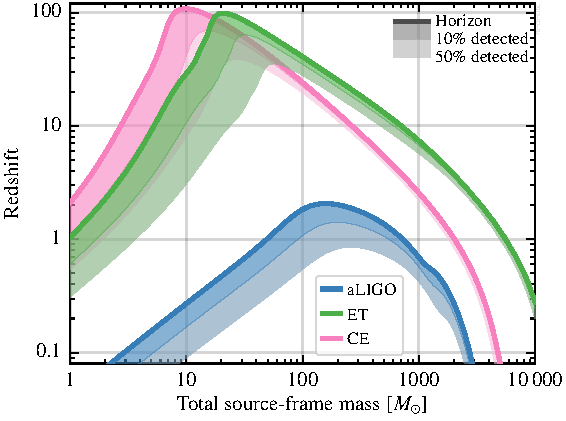
\includegraphics[width=0.6\textwidth]{Figures/gw_horizons_reduce.pdf}\qquad\qquad
% \hspace{-0.09\textwidth}
%  \includegraphics[width=0.4\textwidth]{Figures/waterfall_ET+2CE_maxspin0_q1.pdf}
 \caption{\small Astrophysical reach  for equal-mass, nonspinning binaries  for Advanced LIGO, Einstein Telescope and Cosmic Explorer. 
%Right: lines of constant signal-to-noise ratio in the  (total mass, redshift)  plane, for a network of one ET and two CE detectors. The curves shown assume equal-mass binary components.
}
\label{fig:gw_horizons}
\end{figure}


For NS-NS binaries, whose  total mass is around $3\,\Msun$,  ET will reach $z\simeq 2-3$; by comparison, the NS-NS binary GW170817 was at $z\simeq 0.01$ and, at final target sensitivity, 2G detectors should reach $z\simeq 0.2$.
The corresponding detection rates will be impressive, of order 
$O(10^6)$ BH-BH and $O(10^5)$ NS-NS
%$10^5-10^6$ BH-BH and NS-NS 
coalescences per year; depending on the network of electromagnetic
facilities operating at the time of 3G detectors, over a few years one might
collect $O(10^2-10^3)$     NS-NS GW events with  observed electromagnetic
counterpart. The signal-to-noise ratio of many of these events will be huge,
even for events at cosmological distances.


\emph{The combination of distances and masses explored, sheer number of detections, and detections with very high signal-to-noise ratio will provide a wealth of data that have the potential of triggering revolutions in astrophysics, cosmology and fundamental physics.} 


Beside coalescing binary systems, ET will be able to detect several other kinds of signals, such as stochastic backgrounds of GWs, signals from isolated pulsars, or supernovae, with a sensitivity that improves by orders of magnitude compared to 2G detectors.
Many of the possible achievements of ET, and other planned 3G detectors like Cosmic Explorer in the U.S., are only possible through gravitational waves. For others, GW detectors are complementary to  facilities exploiting electromagnetic radiation  or other messengers, such as neutrinos and cosmic rays. The combined observations through GWs, electromagnetic signals, neutrinos and/or cosmic rays, will give us a multi-messenger picture of many phenomena of the Universe.
Schematically, we can identify the following main items as part of the ET science case:

%\vspace{2mm}

\begin{itemize}
\item Astrophysics:
  \begin{itemize}
   \item black hole properties: origin (stellar vs. primordial), evolution, demography;
   \item neutron star properties: interior structure (QCD at ultra-high densities, exotic states of matter), demography;
   \item multi-messenger astronomy: nucleosynthesis, physics of jets, cosmic rays accelerations, role of neutrinos;
   \item detection of new astrophysical sources of GWs: core collapse supernovae, isolated neutron stars, stochastic background of astrophysical origin.
  \end{itemize}
\item Fundamental physics and cosmology:
  \begin{itemize}
   \item the nature of compact objects: near-horizon physics, tests of no-hair theorem, exotic compact objects;
 % \item Tests of  General Relativity (post-Newtonian expansion, strong field regime, no-hair theorem, ...)
  \item dark matter: primordial BHs, axion clouds, dark matter accreting on compact objects;
  \item dark energy and modifications of  gravity on cosmological scales;
   \item stochastic backgrounds of cosmological origin and connections with high-energy physics (inflation, phase transitions, cosmic strings).
  \end{itemize}
\end{itemize}

% \vspace{2mm}\noindent
It should  be stressed, however, that many questions cross the borders between  domains outlined above. For instance, understanding whether the BHs observed by GW detectors are of stellar or primordial origin obviously has an astrophysical interest, but a primordial origin would have deep consequences on  our understanding of early Universe physics, inflation, etc., subjects that belong to the domain of cosmology and of fundamental physics. As another example, determining the equation of state in the core of neutron stars is of great importance both in astrophysics and for understanding the theory of strong interactions, QCD, in the regime of ultra-high  density, where phase transitions can take place.
 
In the following we briefly discuss some of the science that ET will be able to address\footnote{For more
detailed information on the ET science case and full refereences
the reader is referred to M.~Maggiore \textit{et al.}, `Science Case for the Einstein Telescope', \url{https://arxiv.org/abs/1912.02622}.}.

%\cite{Maggiore:2019uih}.

%\section{Astrophysics}\label{sec:astrophy}

\section{Black hole binaries}\label{sect:Blackholebinaries}

Observationally, BHs have been first identified through X-ray binaries - binary systems in which a BH accretes matter from a companion star. The remarkable GW detections of Advanced LIGO/Virgo in the O1 and O2 runs have then revealed a whole new population of stellar-mass binary BHs with much higher masses, $O(20-80) \Msun$.
With BH-BH and BH-NS coalescence, 3G detectors will explore the Universe to
depths that go well beyond  what can be reached by electromagnetic observations
not only of single astrophysical sources, but even of whole
galaxies.\footnote{To understand how this is possible, it is useful to recall
that a BH-BH coalescence such as the first  detected event, GW150914, converted
into GWs an energy of  $3 \Msun c^2$  in just the last few milliseconds of the
coalescence. The peak luminosity of the event,  $3.6\times 10^{56}\, \mathrm{
erg/s}$, or  $200\, \Msun c^2/{\mathrm{s}}$, was an order of magnitude  larger than
the estimated combined electromagnetic luminosity of all star and galaxies in
the observable Universe!} \emph{ET will uncover the  full population of
coalescing stellar and intermediate mass BHs in the Universe, over the whole
epoch since the end of the cosmological dark ages.}
This will allow ET to answer several key questions about the origin and evolution of BH-BH systems. For instance:

%\vspace{1mm}\noindent
(1) The  observations of BH-BH binaries  across the whole epoch of star formation would contain evidence,  accessible in no other way, of the cosmic history of stellar evolution, including the earliest populations of stars formed in the Universe.   

%\vspace{1mm}\noindent
(2) The observations of BH-BH binaries probe the physics of BH formation in situations which lead to mergers.  ET will provide some events with extraordinarily well-measured properties, alongside large samples of mergers from which statistical population characteristics can be extracted.   
   
%\vspace{1mm}\noindent
(3) By comparing the redshift dependence of the BH-BH merger rate with the cosmic star formation rate it will be possible  to disentangle the contribution of BHs of stellar origin from that of  possible BHs of  primordial origin. 
\emph{Showing that at least a fraction of the observed BHs are of primordial origin would be a discovery of fundamental importance not only in astrophysics but also from the point of view of fundamental physics. }

%\vspace{1mm}\noindent
(4) The discovery of luminous quasars at redshift as large as $z\sim 7$ suggests
the existence, at redshifts $z>7$, of a population of `seed' BHs in the range
$(10^2-10^5) \msun$, from which supermassive BHs have grown through gas
accretion.   ET has the sensitivity necessary to detect  BH binary systems
containing  a  BH with mass between  $O(10^2)\,   \Msun$ and  a few times
$10^3\,\Msun$. \emph{Discovering BHs in this mass range and understanding their role as seed BHs would provide the key to understanding stellar and galactic evolution.}

   
\section{Neutron stars} 

%cold, dense matter and NSs
Neutron stars  are extraordinary laboratories for studying the fundamental properties of matter under conditions far from the realm accessible to experiments and first-principles theoretical calculations. In NSs, intense gravity compresses matter to several times the density of an atomic nucleus. Predicting the composition of such matter and the multi-body interactions that provide the pressure to prevent collapse to a BH requires large extrapolations from known physics, and has been a longstanding scientific frontier.   Neutron stars  provide a unique window onto the behavior of QCD, the fundamental theory of strong interactions, in a regime complementary to the higher temperatures and lower baryon densities accessible in collider experiments that probe the quark-gluon plasma. 

The fundamental properties of NS matter give rise to characteristic imprints in the GW signals from NS, both in  binary coalescences and in the GW signal from individual asymmetric NSs, making GWs unique probes of subatomic physics in unexplored regimes. A 3G GW detector with a high sensitivity and large frequency bandwidth such as ET will be critical to shed light on important fundamental physics questions. 
%In particular:

%\begin{figure}[t]
% \centering
% \includegraphics[width=0.40\textwidth]{Figures/NS_Pie.pdf}\qquad\qquad
%  \includegraphics[width=0.48\textwidth]{Figures/phase_diagram.pdf}
% \caption{\emph{Left}: Conjectured interior structure of a neutron star.  \emph{Right}:
%Matter encountered in neutron stars and binary mergers explores a large part of the QCD phase diagram in regimes that are inaccessible to terrestrial collider experiments. (credit: Sanjay Reddy)}
%\label{fig:NSs}
%\end{figure}

\subsection{Coalescing neutron star binaries} 

With 2G detectors, the first observed NS-NS coalescence
GW170817 demonstrated that useful limits on the NSs' tidal deformability, a characteristic parameter that depends on the properties of matter in their interiors, could be extracted from the inspiral part of the GW signal.%~\cite{TheLIGOScientific:2017qsa}. 
However, despite the proximity of GW170817, the inferred constraints on the equation of state of NS matter~\cite{Abbott:2018exr}
are too weak to discriminate between all realistic models, nor do they offer 
new insights about the possibility of phase transitions (e.g. to a deconfined quark phase) in the inner core.
%~\cite{Hebeler:2010jx,Gandolfi:2011xu,Tews:2018kmu}. 
To determine in detail the nature of matter and interactions in NS interiors requires measuring tidal deformability with an order of magnitude higher accuracy. In addition, such high-fidelity measurements must be obtained for a population of NSs spanning a wide range of masses to map out the parameter dependencies and identify potential signatures of phase transitions. Both can be achieved with ET, which will detect a huge number of NS-NS and NS-BH coalescences per year as quantified above, and will observe their signal with up to tenfold higher accuracy. 

A further unique capability of 3G detectors such as ET is the possibility of exploring in detail the signal after the inspiral part of the coalescence, which, for NS-NS binaries, is at frequencies too high for 2G detectors, but will be within the bandwidth of ET for NS-NS binaries within a few hundreds of Mpc. Witnessing the tidal disruption of a NS  will yield further insights into the properties of NS matter under extreme gravity, and tracking the violent collision of two NSs and its aftermath will provide an exceptional window onto fundamental properties of matter in a completely unexplored regime, at higher temperatures and yet greater densities than encountered in individual NSs. 

The coalescence events of NS-NS and NS-BH systems also have key significance as the principal production site of elements heavier than iron in the cosmos. Heavy elements can be synthesized from the neutron-rich material expelled during the merger or tidal disruption of NSs or through winds from the remnant accretion disk. The subsequent radioactive decay of the freshly synthesized elements leads to an electromagnetic transient known as a kilonova. Multi-messenger observations of a large sample of NS-NS binaries will provide the unique opportunity to study heavy element formation at its production site, to determine how the initial conditions of an astrophysical binary system map to the final nucleosynthetic yields, and the extent to which different NS-NS binary progenitors contribute to the cosmic abundances over time.

\subsection{Continuous waves from spinning neutron stars}

A spinning NS, isolated or in a binary system, if asymmetric with respect to its rotational axis, can also emit continuous semi-periodic GWs. Such asymmetry can derive from frozen deformations produced right after its violent birth, from a strong enough inner magnetic field, or from non-axisymmetric motions or density perturbations. 
No continuous gravitational wave signal has so far been observed  by Advanced LIGO/Virgo.
\emph{The detection of continuous GWs from NS by ET would be a fundamental breakthrough, that would provide   clues about  the condition of formation of isolated NS,  their spin, thermal evolution and magnetic field. Furthermore,  observing such signals with ET's exquisite sensitivity would again give information on the inner structure of NS and on the corresponding aspects of nuclear and particle physics, such as the existence of exotic matter in the NS core.} 
The maximum degree of deformation that a NS can sustain depends on the equation of state: for standard equations of state the maximum value of the ellipticity is $\epsilon_{max} \sim 10^{-6}$, but for exotic objects, containing hyperons or quark matter, is expected to be much higher, $\epsilon_{max}\sim 10^{-4}-10^{-3}$. In practice, it is difficult to predict the actual deformation of  a specific NS, that can depend on the star's history and could be well below the maximum sustainable value.   ET will be sensitive to ellipticities of the order of few times  $10^{-10}$ for the nearest millisecond pulsars, and of $\sim 10^{-6}-10^{-7}$ for young pulsars. 
 It is quite impressive to realize that detecting GWs due to an eccentricity of, say, $\epsilon=10^{-7}$ in a NS means that we would detect the effect  due to a ``mountain'' on a NS, with a  height of about $10^{-7}\times 10\, \mathrm{km}=1\, \mathrm{mm}$!  %(or $10^{-2}$\,mm, for $\epsilon=10^{-9}$).

The maximum distance at which a continuous wave source would be detected
%,  assuming that the source spin-down is dominated by the emission of GWs and an observation time of a few years, 
depends on both the ellipticity and the rotational frequency of the NS. For instance,  a neutron star spinning  at 50\,Hz (and then emitting a continuous GW signal at 100\,Hz) would be detectable by ET  in the whole Galaxy as long as its ellipticity is larger than $10^{-7}$. 
Very  fast spinning  and highly distorted neutron stars,  such as newborn magnetars produced in core collapses or as post-merger remnants of coalescing binaries, could lead to detectable emission at even higher frequencies. In this case the signal can only be observed for a shorter time, since these objects  
are characterized by a very high spin-down and the signal frequency eventually leaves   the detector sensitivity band within a  few days. However, at birth they could have ellipticities as large as $10^{-3}$ so,  even taking into account uncertainties in the data analysis due to the very large initial parameter space (initial frequency, spin-down, braking index), these objects could still be detected out to distances of  tens of megaparsecs.
 

\section{Multi-messenger astrophysics: synergies with other GW detectors and electromagnetic/neutrino observatories}
\label{sec:MM}
%\newcommand{\TOFIX}[1]{\textcolor{red}{#1}}
%\subsection{Synergies with other GW detectors and multi-messenger astrophysics}


ET, with its triangular configuration corresponding to three nested interferometers, is designed to have an extraordinary science output even when operated as a single GW detector. However, a further enhancement of its capabilities will take place when making use of  the synergies with other detectors that could be operating at the same time.

\subsection{Networks of 3G gravitational-wave detectors}

The first obvious synergy is with other GW detectors of third-generation, like the Cosmic Explorer (CE) under study in the US. The most important improvement of a network of three 3G detectors, compared to a single detector, concerns the accuracy in the localization of the sources. For the continuous GWs emitted by spinning NSs a single ET detector  already provides a very accurate parameter estimation - including position - thanks to the very specific modulation of the signals due to Doppler effect induced by the Earth motion.   For coalescing NS-NS binaries a single ET detector (especially in the ET-D configuration with low frequency cutoff in the sensitivity curve) still has some localization capability since, for a low-mass system such as a binary NS, the signal can stay in the detector bandwidth for a long time,  of order of a few days, and again the modulation due to  the Earth motion allows us to localize the source. In this case  an average angular resolution would be around  $150\deg^2$\, for a binary NS at $z=0.1$, but can become of order of just a few $\deg^2$ for the best localized 
sources.
%~\cite{Zhao:2017cbb,Chan2018}. 
No significant localization will be available for BH-BH and BH-NS binaries, that because of their higher total mass will stay in the detector bandwidth for a much shorter time.
A  network of three GW detectors, in contrast, will have quite  good localization accuracy  for all types of binary coalescences; for example a large fraction of NS-NS binaries will have sky localization smaller than 1 deg$^2$ up to $z=0.5$. 
In terms of science output, this means that a 3G detector network will be able to provide good localization information to electromagnetic telescopes, for the search of electromagnetic counterparts. 
%(in the case of systems involving NS; no electromagnetic counterpart is expected for BH-BH systems). 


On the other hand, the different sensitivity curves planned for  ET and CE imply that, from other points of view, these detectors will be complementary. For instance,  as can be seen from  Fig.~\ref{fig:gw_horizons}, ET will be  able to detect heavier systems, with total masses  higher than $10^3~\Msun$ (thanks to its sensitivity in the low frequency regime), while CE has a greater reach  for light systems such as NS-NS binaries.
The different sensitivity curves also mean that, for a given astrophysical system, the signal-to-noise ratio is accumulated differently in ET and in CE, providing complementary information.



\subsection{Joint gravitational and electromagnetic observations}
\label{sec:MM-EM}

The discovery and electromagnetic follow-up of GW170817 showed the enormous potential  of gravitational-wave observations for multi-messenger astrophysics. The gravitational-wave observations combined with the results from the extensive multi-wavelength observational campaign (still undergoing) had a huge impact on our knowledge of the physics of compact objects, relativistic jets, nucleosynthesis, and cosmology. Identifying the electromagnetic signatures of the gravitational-wave sources enables to maximize the science return from a gravitational-wave detection.  
Several future observatories, with a large involvement of the European community, will have strong synergies with ET. SKA, LSST, the THESEUS mission concept, and CTA will be able to observe large regions of the sky from the radio, optical to the X-ray and very high energy, going to deeper sensitivity than current observatories; a 40-meter class telescope such as ELT and a satellite like ATHENA will be able to characterize the source in the optical and X-ray band respectively. 

The ET lower frequency capability enables 
the accumulation of a significant signal-to-noise ratio before the merger, making possible an early detection and warning for the electromagnetic/neutrino followup. Requiring a signal-to-noise ratio of $\geq\,12$ and a sky localization smaller than 100\,deg$^2$, ET can send an early warning alert between 1 and 20 hours before the merger (with the mean of the distribution at about 5\,hours) for signals at 40\,Mpc. 
%\cite{Chan2018}. 
At 200\,Mpc, about 30\% of the detectable signals would accumulate enough SNR for early warning between 1 to 6 hours prior to the merger; about 10\% of the detectable sources within 400\,Mpc can still be announced with an early warning smaller than 1\,hour. This enables the detection of early electromagnetic emission, which is fundamental to understand the physics of the engine and the merger remnant.



%\subsubsection{Nucleosythesis and kilonova emission}
%The cosmic origin of elements heavier than iron has long been a mystery. The thermal emission in the ultraviolet, optical, and near-infrared detected with GW17017 is consistent with kilonova emission powered by the radioactive decay of  heavy nuclei synthesized in the merger ejected by the rapid neutron capture process (r-process). The kilonova associated with GW17017 provided the first observational test to theoretical models which predict r-process nucleosynthesis during  binary neutron star mergers. Spectra, emission timescale and color evolution are directly related with the amount of mass ejected during and after the merger, the ejected mass, velocity, the opacity of the sythetized elements, and the merger remnant. In contrast with supernovae, the spectra do not show narrow lines, but results in an initial featureless smooth optical spectrum due to the blending of lines coming from the high expansion speed of the photosphere, followed by broad absorption features in the near infrared due to lanthanide nuclei synthesized in the merger ejecta. On the basis of the merger rate estimated using the LIGO and Virgo observations and the amount of ejected mass estimated by the kilonova observations, binary neutron star mergers are now understood to be a major channel of r-process production, able to explain the r-process abundances in the Milky Way stellar population. However, it is still uncertain the role of rare classes of supernovae, such as the collapsars associated with long gamma ray bursts, which are expected to be an additional significant source of r-process elements \cite{Siegel2019}. Only a larger sample of kilonova, possibly extending to larger distance, will enable to probe the details of the kilonova emission mechanism, the role of the neutron/black hole merger, and the formation of heavy elements along the cosmic history. 
%
%When ET is expected to observe the sky, LSST will operate as a wide field-of-view survey able to detect kilonova emission up to 800 Mpc. Up to the same distance photometric and spectroscopic characterization will be possible using ground-based 30--40 m telescopes such as TMT and ELT, and the space telescope JWST.  The binary neutron star mergers detectable in this volume are order $10^3$ per year;  for a large fraction of these sources the error box in the  gravitational-wave localization at a distance $> 400$ Mpc  will make  difficult to identify the optical counterpart  among many optical transient contaminants. Still, a significant number of joint GW/electromagnetic detections are expected, in particular if there will  be a detection with an accurate sky localization at high-energy (see the following subsection). For joint gravitational wave/kilonova detection, the precision of parameter estimation for the progenitor system (total mass, mass ratio, spin, and neutron star tidal deformability) and the detection of the signal from the merger remnant made possible by ET represent an unprecedented opportunity to understand the physics governing the kilonova emission, and the nature and equation of state of neutron stars.

%\subsubsection{Relativistic astrophysics and short gamma-ray bursts}

A single ET detector, even in the absence of good source localization, will still be able to perform joint observations with gamma-ray burst (GRB) detectors, through  the observation of a temporally coincident GRB. In turn, this  can  allow for the measurement of the redshift of the source when the high-energy satellite is capable to precisely  localize it. Indeed, GRB satellites such as "Swift" regularly alert ground based spectrographs to obtain the redshifts of the host galaxies of the detected GRBs. 

%Approximately two seconds after GW170817, the Fermi space telescope detected a weak short-duration gamma-ray burst, GRB170817A. Even if it showed the classical observational features that led to classify it as a short GRB, its total gamma-ray energy of about $10^{46}$ erg was many orders of magnitude smaller than the typical energy of any GRB observed before. Nine and sixteen days after the  GW observation of the merger, X-ray and radio emissions were also detected. Over longer timescale the radio, optical, and X-ray observations showed a slow achromatic flux increase until about 150 days before starting to decline. High-resolution radio observations were able to constrain the source size and to show a source displacement consistent with the launch of a jet which successfully breaks through the ejecta developing an angular structure; a narrow ultra-relativistic jet surrounded by less-collimated and slower material. The  structured jet was observed off-axis (i.e. the observer was misaligned with respect to the collimated ultra-relativistic jet). However, while multi-wavelength observations over two years have built a broad consensus about the interpretation of the non-thermal afterglow emission, the origin of the extremely faint prompt gamma-ray emission observed far from the jet core is still under debate; a gamma-ray emission arising from the slower part of the jet or a gamma-ray emission due to shock breakout from thermal energy in a cocoon produced by the jet-ejecta interaction.


The discovery of the gamma-ray emission  associated with GW170817 and the following afterglow observations significantly improved our knowledge of short GRB jets. However, only a detector such as ET will provide the unprecedented capability to completely probe short GRB jet properties by exploring up to high redshift a large population of neutron star mergers observed perpendicular to the orbital plane (on-axis) and off-axis. Mission concepts such as THESEUS will be able to detect $20-40$ on-axis short GRB/year with a localization accuracy of $1-5$ arcmin up to a redshift $z\simeq 5$.
%~\cite{Stratta:2017bwq}.  
After each detection, the rapid alert system will enable to point ground-based spectrographs, such as the ones in ELT and satellites such as ATHENA. THESEUS will give the precise position of the source, and ET and the multi-wavelength follow-up will allow us to connect detailed information of the progenitors and merger remnant properties to the jet and environment properties. It will be possible to build a statistical sample of binary neutron star mergers  able to probe the shape of the jet structure, if it is universal, and investigate what is the typical opening angle for short GRBs. It will be possible  to constrain the  luminosity function  of short GRBs and its relation to the jet structure and the intrinsic luminosity evolution, and to understand what is the efficiency of the jet to break through the material surrounding the NS-NS mergers. Finally, we will understand  the role of NS-BH binaries as progenitor of short GRBs. ET will be crucial to identify the nature of the binary neutron star merger remnant (black-hole, unstable or stable neutron star) and how this is connected to the short GRB central engine and afterglow properties.

%ET will guarantee that instruments such as THESEUS will have a gravitational-wave detection for each detected on-axis GRB. Over a few years, it will be possible to build a sample of tens to $O(100)$  joint detections with luminosity distance measured by gravitational-waves and  redshift measured by ground-based telescopes, such as VLT and ELT. These detections will provide precise measurements of the Hubble constant, helping to break the degeneracies in determining other cosmological parameters obtained by CMB, SNIa and BAO surveys, and to study the nature of dark energy~\cite{Belgacem:2019tbw};  see section~\ref{sec:cosmos} for details.
%
%The detection of a faint off-axis gamma-ray signal such as the one observed by Fermi and INTEGRAL for GW170817, will be difficult for present and the planned future detectors at distances larger than 100 Mpc. However, a fraction of NS-NS merger are expected to produce long-lived neutron stars. In this case, soft X-ray transient can be powered by the new-born neutron star spin-down emission. Even if never observed so far, this emission is expected to be powerful and nearly isotropic \cite{Metzger2014,Siegel2016}. Large field of view instruments, such as the one on board of THESEUS, will allow to detect  the brighter emissions up to 1 Gpc, thereby increasing the numbers of joint GW/electromagnetic detections to a few hundreds per year. 


%\subsubsection{Multi-messenger observations and core collapse supernovae}
%
%Despite the remarkable progress of the theory, the explosion mechanism of supernovae is still an open question, and being able to measure the dynamics of matter at the onset of the phenomena would bring invaluable information to the understanding of the physics of gravitational core collapse. 
%What is fairly known since the 1970's is the role of the neutrinos in the explosion mechanism. During collapse, the stellar core becomes opaque to neutrinos, producing a degenerate sea of trapped neutrinos within it, which subsequently diffuses out of the core on a timescale of order tens of seconds as the nascent proto-neutron star  cools and deleptonizes.
%The three-flavor neutrino flux emanating from the proto-neutron star could power itself a core collapse supernova  via neutrino heating on delayed timescales of order one second. This phenomena is central to most models today, with the exception of models of rare events involving significant rotation, which may be powered magneto-hydrodynamically and where the dynamics proceeds  on shorter timescales. 
%
%Core collapse SNe are not a guaranteed source for ET. A general consensus from all modern numerical simulations is that the expected GW signal is weak (GW released energy of the order of $10^{-9}$~$M_\odot c^2$). Furthermore, the likely diversity of the GW emission mechanisms that are at play in SN explosion makes quite difficult to use matched filtering techniques for digging the signal out of the noise, contrary to what can be done with coalescing binaries or spinning neutron stars. As a consequence,
%the detection of a core collapse supernova GW signal is very challenging
%and the discovery horizon of the current 2G detectors is limited to our galaxy. The expected galactic rate of type II/Ib supernova is also rather small (~1 per 30 years). ET will extend the reach to our galactic neighborhood, so that the expected rate is such that, while detection is not assured, still it is a realistic possibility.  
%
%However, a detection of the GWs emitted in core collapse would be a milestone, revealing the inner mechanisms of core collapse and opening remarkable perspectives  in multi-messenger astronomy. In particular,
%the neutrino emission which will be in coincidence with the GW emission, within few milliseconds, should be detected by the current and future low energy neutrinos detectors (Super-K/Hyper-K, DUNE, JUNO, IceCube, the LVD, Borexino and KamLAND) with a higher signal to noise ratio than the GW signal and a very precise time resolution (few milliseconds) which is a fundamental information to search for a  signal with low 
%signal-to-noise ratio  in the GW data. The false alarm rate of GW searches can be significantly improved with the temporal localization given by the neutrino signal. Furthermore, there exists a strong correlation between the GW and neutrino signals as they are produced at the same interior location and will be powered by the downward accretion plumes associated with hydrodynamic instabilities present in the post-shock flow. These plumes and instabilities will modulate both signals.
%If the signal is likely to remain short (of the order of 1~s), it is expected to be wide band (from few Hz up to several kHz), with very different mechanism in each frequency band. The low frequency and high frequency ET conception design is very well suited for detecting such kind of GW signal.
%
% 

\subsection{Neutrinos and cosmic rays}

Shock-accelerated particles (protons and nuclei) interacting with matter and photons produce neutrinos. The astrophysical sources of gravitational-wave transient signals associated with gamma-ray bursts (GRBs), soft gamma-ray repeaters (SGRs), and core-collapse supernovae are expected to emit neutrinos. While gravitational waves produced by the bulk motion of matter carry information on the astrophysical source dynamics, neutrinos give direct information on interactions between accelerated particles with matter and radiation surrounding the sources. GWs and neutrinos probe the innermost regions of the source typically opaque to the electromagnetic emission. GRBs and SGRs are expected to emit high energy cosmic neutrinos (HEN) from MeV to PeV. In the GRBs, TeV-PeV HENs are expected to be produced in the baryon-loaded jets during the prompt gamma-ray emission, and PeV-EeV HENs during the afterglow phase. In SGRs, the HEN production is expected from protons accelerated by the sudden magnetic reconfiguration. 

When ET will be operational, the upcoming multi-cubic-kilometer neutrino detector KM3NET, and the 10\,km$^3$ facility in the Southern hemisphere IceCube-Gen2 are expected to observe the sky. The sensitivity of the neutrino detectors will make the simultaneous detection of neutrinos and GWs from on-axis short GRBs possible. The high-energy neutrinos would serve as a powerful probe of cosmic-ray acceleration in GRBs and of the physics of relativistic jets associated with NS–NS and NS-BH mergers. For long GRBs and SGRs, the joint detection is less likely and more uncertain. Some models predict that GRBs produce Ultra-High Energy Cosmic Rays (UHECR). In the case of cosmic ray, the astrophysical source identification is complicated by the cosmic ray deflection and the time delay between the arrival of cosmic rays and photons, GW and neutrinos imparted by magnetic fields in the galaxy hosting the source, our Galaxy, and in the intergalactic medium. In this context, ET together with gamma-ray observatories, such as Fermi, HESS, MAGIC, VERITAS, Fermi, CTA and neutrino detectors will make it possible to probe the GRB population, their progenitors, and the jet properties and composition. This will be crucial to probe the role of GRBs as possible sources of UHCRs.

Core-collapse supernovae emit low-energy neutrinos, as proved on February 23, 1987, when neutrinos with energies of a few tens of MeV emitted by the supernova SN1987A, exploded in the nearby Large Magellanic Cloud, were recorded simultaneously by the Kamiokande-II, IMB, and Baksan detectors a few hours before its optical counterpart was discovered. Simultaneous detection of GWs and neutrinos from core collapse of massive star would open remarkable perspectives in multi-messenger astronomy. They are unique probes to reveal the inner mechanisms of the explosion, the dynamics of the remnant (possible a newborn neutron star) and the physics of the post-shock region. The current and future low-energy neutrino detectors Super-K/Hyper-K, DUNE, JUNO, IceCube, the LVD, Borexino, SNO+ and KamLAND are expected to detect neutrinos from the core-collapse SNe, whose GW signal will be detectable by ET. The very short time delay among GW emission and neutrinos (expected to be less than a few milliseconds) represents also a fundamental information to search for signals with low signal-to-noise ratio in the GW/neutrino data.

\subsection{Multi-band GW observations with LISA}

Another potential very interesting synergy could take place with the space interferometer LISA, should ET be operational  by the time that LISA will take data (launch scheduled for 2034, operational from 2036 for a nominal duration of four years), or up to a few years  after the end of the mission. This would allow multi-band GW observations, i.e. the observation of GW signals in widely different frequency bands. In particular, from the rate of BH coalescences inferred by the Advanced LIGO/Virgo O1 and O2 runs, 
we expect that LISA, in a 4\,yr mission, will detect several tens of stellar-mass BH-BH binaries.
%we know that  LISA will detect at least $O(100)$ stellar-mass BH-BH  binaries during their inspiral phase, up to $z\simeq 0.4$.
%~\cite{Audley:2017drz}.   
Months to years later, several of these events will cross into the ET window, where they will coalesce. For instance, the first observed GW event, GW150914,  
would have been detected by LISA a few years before coalescence,
%~\cite{Sesana:2016ljz}, 
if  at that time LISA had already been  in orbit.


Multi-band observations would have many benefits: a joint LISA-ET detection would provide
sky localization of the source with an error of only a few square degrees, and 
would make it possible to alert telescopes and look for an electromagnetic counterpart, both  in the pre-merger and post-merger phases (which in principle is not expected for BH-BH coalescences, but could be present in BH-NS binaries); it
would improve parameter estimation, reducing the error on the luminosity distance to the source and on the initial spins  and  allowing to measure with extreme precision the sky position, mass and spin of the final BH. LISA and ET observations of such events would be highly complementary; for instance LISA, by observing the long inspiral phase, will measure very accurately the masses of the initial BHs, while ET  would detect  the last few cycles and the merger, and would therefore measure the final masses and spin from the ringdown of the final BH. Consistency tests  between the
inspiral part of the waveform and the merger-ringdown part, of the type performed 
%in \cite{TheLIGOScientific:2016src} 
for the first detection GW150914, would then provide very stringent tests of General Relativity.
%~\cite{Vitale:2016rfr}.
Furthermore, the early warning provided by LISA on particularly interesting events might allow real time optimization of ET  to improve sensitivity to the ringdown signal.
%~\cite{Tso:2018pdv}.

\section{Fundamental physics and cosmology}

The direct detection of gravitational waves has started to give us access to the genuinely
strong-field dynamics of spacetime. This is illustrated in Fig.~\ref{fig:phasediagram}, which shows how 
different kinds of observations (past, current, and future) will give us access to different
regimes, in terms of spacetime curvature $R$ and gravitational potential $\Phi$ (which for binary 
systems can be traded for $v^2/c^2$, where $v$ is the characteristic speed of the binary and $c$
is the speed of light). 

\begin{figure}[t]
\centering
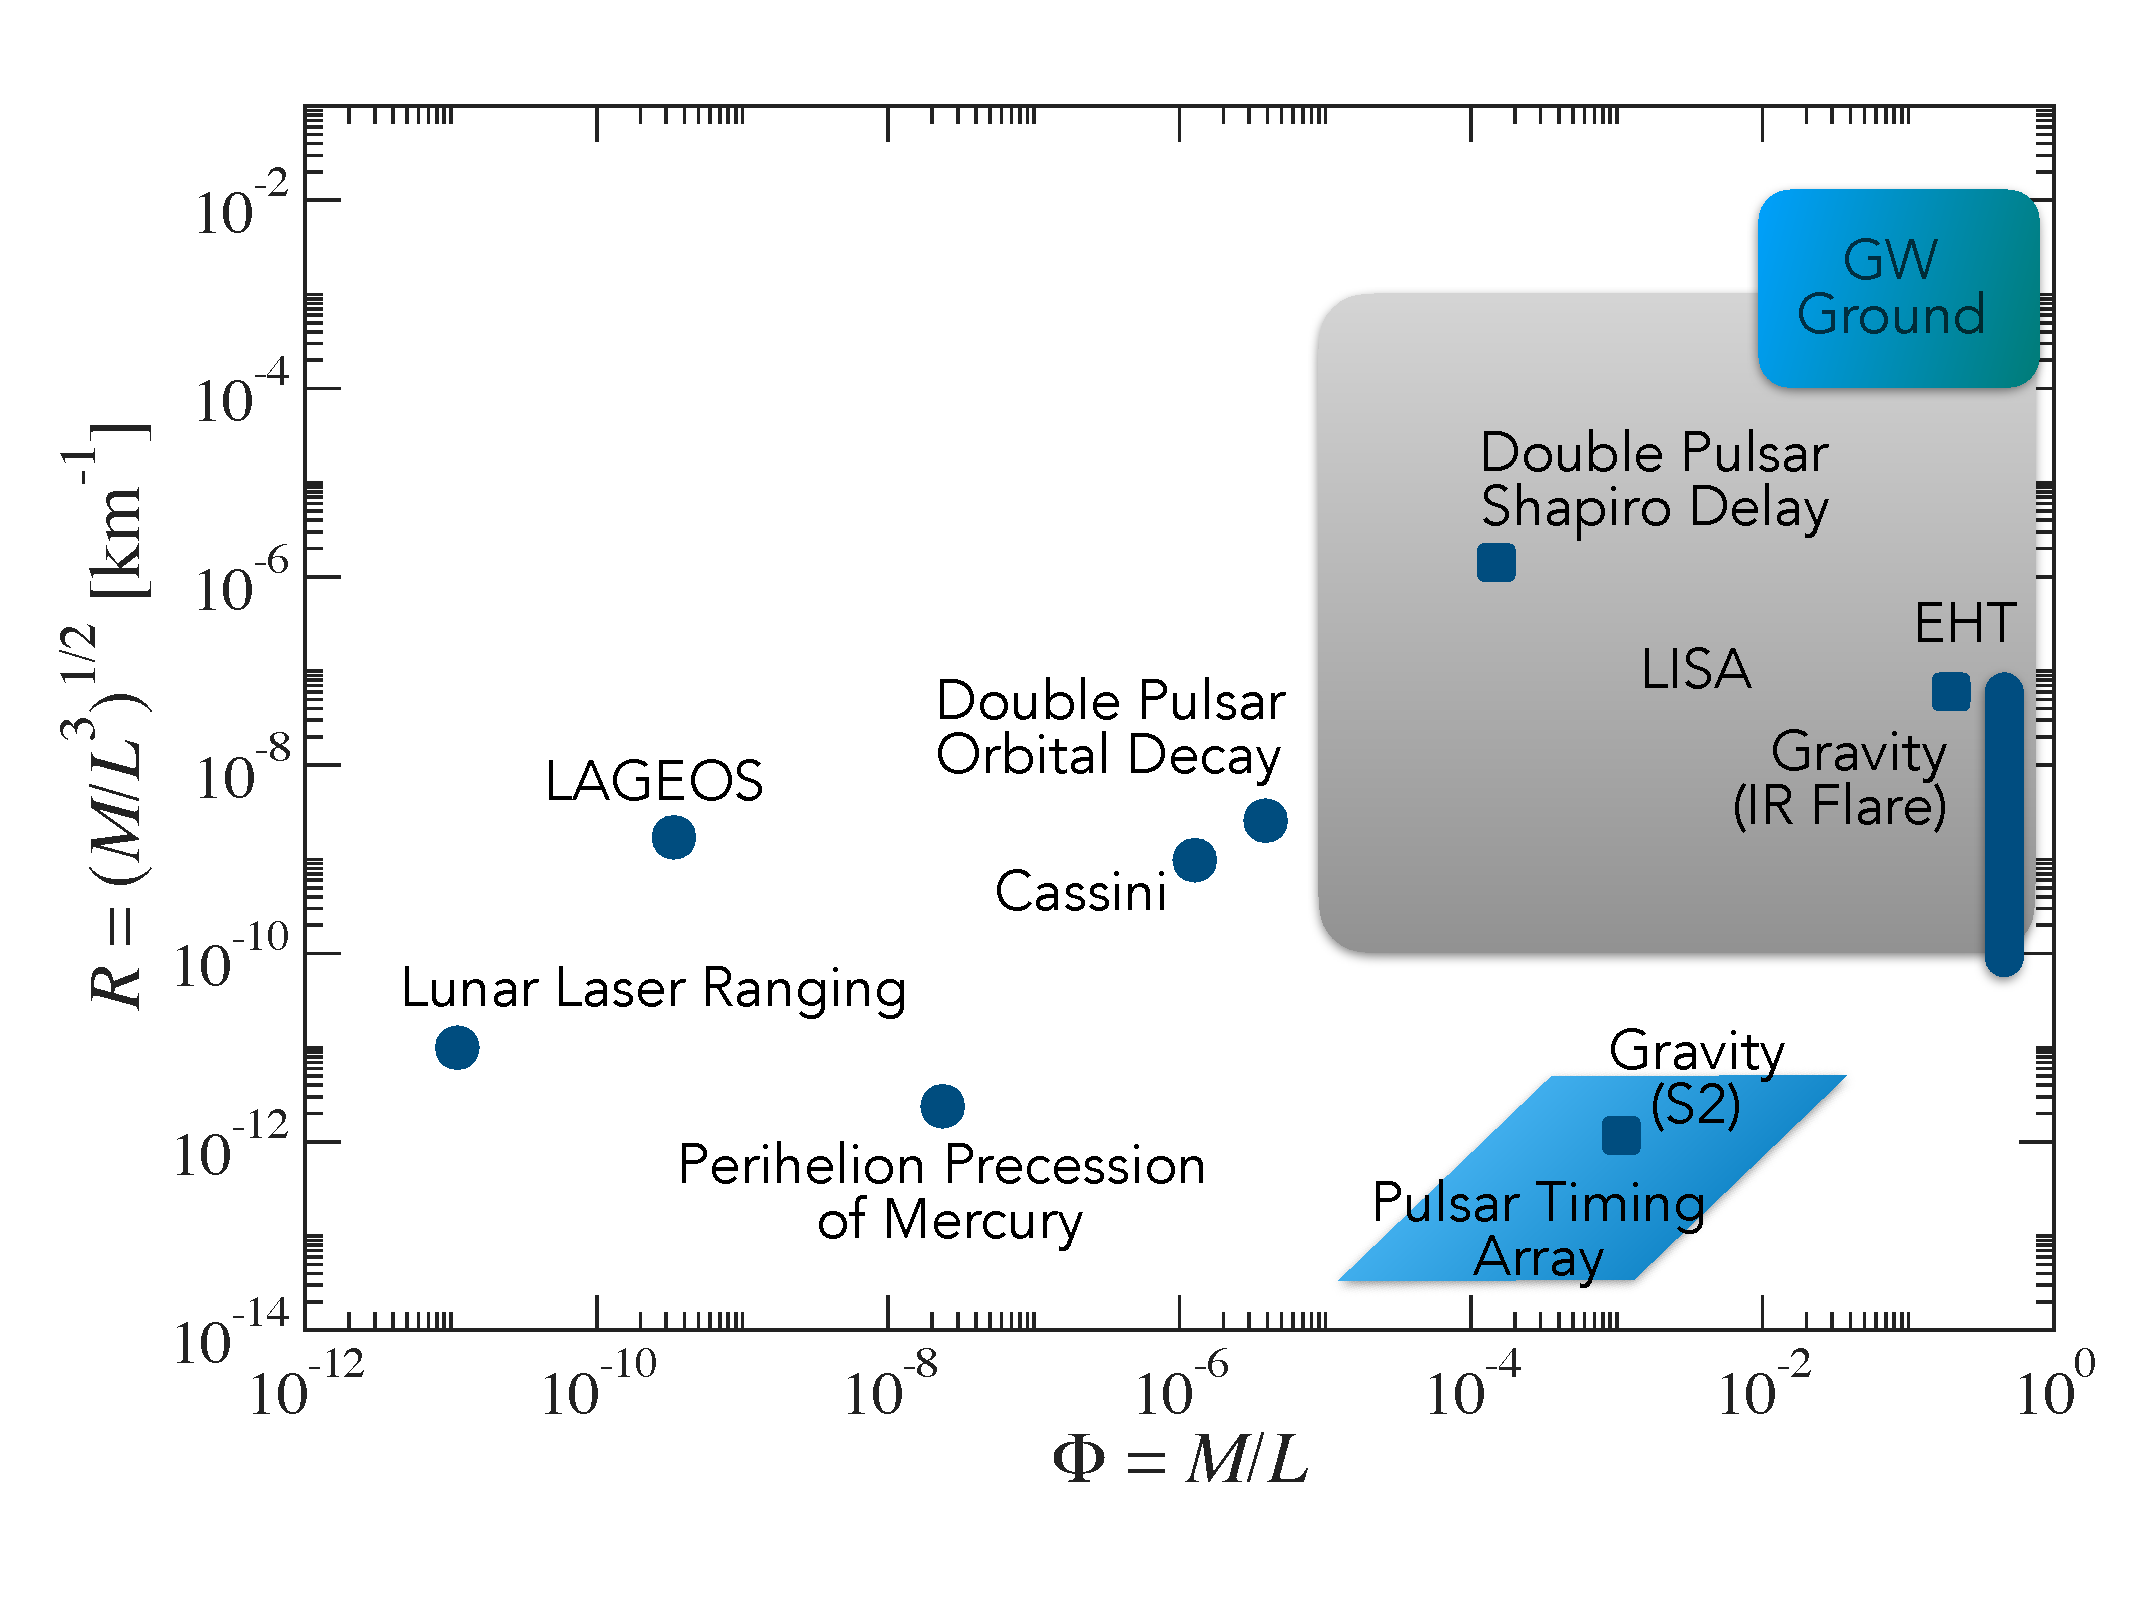
\includegraphics[width=0.8\textwidth]{Figures/ToG2_reduce.pdf}
\caption{\small Probing gravity at all scales: illustration of the reach in spacetime curvature versus potential energy targeted by different  kinds of observations. 
$M$ and $L$ are the characteristic mass and length involved in the system or process being observed. 
The genuinely strong-field dynamics of spacetime manifests itself in the top right of the diagram. The label EHT refers to the Event Horizon Telescope.
Image from the `3G Science Book' by the the GWIC 3G Science Case Team, and the International 3G Science Team Consortium (in preparation, 2020).
%From ref.~\cite{Sathyaprakash:2019yqt}.
}
\label{fig:phasediagram}
\end{figure}

Observations of GWs from binary BH and binary  NS coalescences with Advanced LIGO and Advanced Virgo have enabled us to probe for the first time the regime where both $R$ and $v/c$ are large. By observing the inspiral phase  we could test the predictions of GR (as encoded in the post-Newtonian coefficients) to a precision of about $10\%$.
By observing the full  inspiral-merger-ringdown process of binary black holes, we could perform a first study of the dynamics of vacuum spacetime. 
The observation of the binary neutron star inspiral GW170817 also gave us our empirical 
access to the interaction of spacetime with high-density matter. Because of the large 
distances that GWs have to travel from source to observer, we were able to
strongly constrain possible dispersion that might occur; the latter led to a bound on 
the mass of the graviton of $m_g \leq 5 \times 10^{-23}\,\mbox{eV}/c^2$. These examples
notwithstanding, on the whole the existing detectors lack the sensitivity to put very strong
constraints on possible deviations from Einstein's theory, particularly regarding 
the strong-field dynamics at the source, corresponding to the top right edge of 
Fig.~\ref{fig:phasediagram}. 
The situation will be quite different with Einstein Telescope. One reason is the much 
larger detection rate; especially for the purposes of fundamental physics, information 
from multiple sources can often be combined, and the measurement accuracy on 
common observables  
tends to improve with the square root of the number of detections. 
For example, the post-Newtonian coefficients that govern binary inspiral will be determined with sub-percent to sub-permille accuracy.
However, the fact that
the same GW source will be much louder in ET will also give us access to 
qualitatively new effects. Below we discuss in turn capabilities of ET in 
probing the properties of gravity, as well as unraveling the nature of ultra-compact
objects, with potentially game-changing implications for our understanding of black holes, 
the make-up of dark matter, dark energy, and maybe even quantum gravity itself.



\subsection{Physics near the black hole horizon}%: from tests of GR to quantum gravity}



%\vspace{2mm}
%\noindent
\emph{Testing the GR predictions for space-time dynamics near the horizon}.
Black holes are one of the most extraordinary predictions of General Relativity. They are identified through  their most striking property: in the case of stellar mass black holes, a mass $O(10-100)\,\Msun$ is concentrated in an extremely small volume; for instance, the Schwarzschild radius of a non-rotating BH with mass $10\msun$ is about 30\,km. However, how certain can we be that the massive compact objects that we saw merge with 2G detectors are really the standard black holes of classical General Relativity?

\begin{figure}[t]
\centering
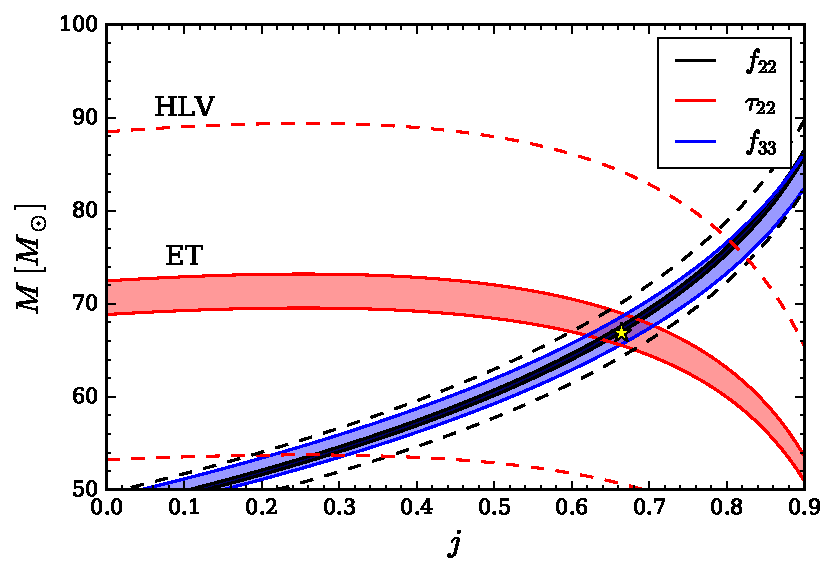
\includegraphics[width=0.7\textwidth]{Figures/3g_ringdown.pdf}
\caption{\small Testing the nature of black holes by using two quasi-normal modes and checking
that the characteristic frequencies $f_{22}$ and $f_{33}$ and the damping time $\tau_{22}$ are consistent
with each other, given that for ordinary black holes these can only depend on two numbers, namely
the final mass $M$ and final spin $j$. The estimates are for the ``ringdown" of the remnant
black hole arising from a binary similar to the source of GW150914. The dashed curves marked HLV 
are the 95\% confidence regions one would obtain from Advanced LIGO-Virgo, while the colored bands
are for ET. The star indicates the true values of $M$ and $j$.
}
\label{fig:ringdown}
\end{figure} 

General Relativity gives detailed and specific predictions on the nature of BHs that a 3G detector such as ET will be able to test. The celebrated no-hair theorem  of GR states that, in  a stationary situation, a BH is determined
by just two numbers: its mass and its spin (plus the electric charge, which however is not relevant in an astrophysical context, where it is quickly neutralized). However, when a BH is perturbed, it reacts in a very specific manner, relaxing to its stationary configuration by oscillating in a superposition of 
quasi-normal modes, which are damped by the emission of GWs. The fact that an elastic body has normal modes is a familiar notion from elementary mechanics. It is however quite fascinating to realize  that a BH, which is a pure space-time configuration, also has its quasi-normal modes. These represent pure space-time oscillations, in a regime of strong gravity, and, in a sense, describe the elasticity of space-time in a most extreme situation, in the region close to the BH horizon. The theory of BH quasi-normal modes is a classic chapter of GR,
%(see \cite{Berti:2009kk,Maggiore:2018zz} for reviews), 
and in particular predicts the spectrum of frequencies and damping times of the quasi-normal modes as a function of the mass and spin of the BH. Highly perturbed black holes arise as the 
remnants of binary BH or NS mergers, and relax to the final stationary BH configuration through GW emission in the quasi-normal modes, in the so-called `ringdown' phase of the coalescence, where the waveform is given by a superposition of damped sinusoids. Indeed, for the first observed BH-BH coalescence, GW150914, the final ringdown phase was just discernable, and was shown to be broadly consistent with the prediction of GR for the value of the parameters inferred from  the inspiral part of the waveform.
%~\cite{TheLIGOScientific:2016src}. 
Fig.~\ref{fig:ringdown} illustrates the difference in the accuracy of such a test between 2G and 3G detectors, for a single source such as GW150914. Furthermore, 
the accuracy of the measurement scales as $1/\sqrt{N}$, where $N$ is the number of detections;
as we saw, ET will detect $N\sim O(10^5-10^6)$ BH binaries, compared to several hundreds expected for 2G detectors.


%\vspace{1mm}
%\noindent 
\emph{Exploring the possibility of exotic compact objects}.
The observation of quasi-normal modes, besides providing a spectacular test of GR in the strong-field, near-horizon regime, could also potentially lead to the discovery of different types of compact objects.
Indeed, various exotic compact objects have been proposed that may act as ``black hole mimickers", such as boson stars, gravastars, etc.
%(see \cite{Cardoso:2019rvt} for review). 
When such  objects are part of a binary system that undergoes
coalescence, they can make their presence known through various possible imprints on 
the GW signal emitted. Already during the inspiral phase, these objects may get tidally deformed in a way that would be impossible 
for a standard, classical black hole. Unlike second generation detectors, ET will for instance be able 
to distinguish neutron stars from boson stars even for the most compact models of the latter.  
Another possibility is that an exotic object could be identified through 
an anomalous spin-induced quadrupole moment, which would again not be accessible with 
current detectors, but measurable with ET to the percent level.
%~\cite{Krishnendu:2017shb}.

If the outcome of a coalescence is different from a BH, this might leave an imprint on  the  ringdown phase, and could be tested by measuring quasi-normal mode frequencies and life-times, as in Fig.~\ref{fig:ringdown}. For exotic compact objects where the modifications take place only at  scales much shorter than the so-called light-ring (as in the case of quantum gravity effects discussed below), the ringdown signal will be very similar to a BH, but after the ringdown has died down, exotic compact objects may continue to 
emit bursts of gravitational waves at regular time intervals, called \emph{echoes}.
%~\cite{Cardoso:2016rao,Cardoso:2017cqb}. 

%\vspace{2mm}
%\noindent
\emph{Signals from quantum gravity?}
Prompted by Hawking's 
information paradox, modifications of the structure of space-time at the horizon scale have been proposed, such as firewalls~\cite{Almheiri:2012rt} and fuzzballs,
%~\cite{Mathur:2005zp}, 
for which the classical horizon is removed through macroscopic quantum effects. 
From a particle physics perspective, one is used to the fact that, at energies $E$ much below the Planck energy scale $M_{\mathrm{Pl}}$, quantum gravity effects are suppressed by powers of 
$E/M_{\mathrm{Pl}}$, and therefore, given that  the Planck scale $M_{\mathrm{Pl}}$ is of order $10^{19}$\,GeV, they are totally unaccessible at accelerators, even in any foreseeable future. Equivalently, at a macroscopic length-scale $L$, quantum gravity effects are suppressed by powers of $l_{\mathrm{Pl}}/L$, where $l_{\mathrm{Pl}}\sim 10^{-35}$\,m is the Planck length. In contrast, near the BH horizon, where the characteristic length-scale $L$ is given by the Schwarzschild radius $R_S$, effects due to quantum gravity  are governed  by a factor  $\log (l_{\mathrm{Pl}}/R_S)$, and can manifest themselves  through a series of echos after the initial ringdown signal,
%~\cite{Cardoso:2016rao,Cardoso:2016oxy,Cardoso:2019apo}, 
emitted with a time delay  $\tau_{\mathrm{echo}}\simeq (R_S/c) \log (R_S/l_{\mathrm{Pl}})$. For instance, for a final object with mass $M=60\Msun$, one has 
$\tau_{\mathrm{echo}}\simeq 16 \tau_{\mathrm{BH}}$, where $\tau_{\mathrm{BH}}\simeq 3$\,ms is the fundamental damping time of a Schwarzschild BH with this mass. Such signals 
 are potentially within the reach of ET, which raises the tantalizing possibility of accessing 
quantum gravity effects at ET.

To summarize, \emph{the transition from second generation observatories to Einstein Telescope
will lead to a qualitative leap in our ability to probe both the nature of gravity in the strong field regime 
and the structure of compact objects, and could even lead to exploring the quantum gravity regime.} 


\subsection{The nature of dark matter}

Understanding the nature of dark matter and of dark energy is one of the crucial problems in astrophysics, cosmology and fundamental physics.  ET will be able to address both questions. 
Observations at ET will allow us to attack the problem of the origin of dark matter from several different angles. Dark matter could be composed, at least in part, of \emph{primordial} black holes in the mass range $\sim 0.1 - 100\,M_\odot$.
%~\cite{Carr:2019hud,Garcia-Bellido:2019vlf,Clesse:2016vqa,Clesse:2016ajp,Garcia-Bellido:2017fdg}. 
Primordial BHs  could be seeded by fluctuations generated during the 
last stages of inflation, which then collapsed in later epochs as a consequence of drops in the pressure of the cosmic fluid, e.g. during the  QCD quark-hadron transition. Their mass distribution depends on the precise model 
of inflation and on the epoch when they  collapsed. The large number of mergers that ET
will see, together with its  ability to access a broad range of masses, would allow us to map the black hole mass distribution
and identify an excess of black holes in certain mass intervals. For black holes with masses well below a 
solar mass, no plausible astrophysical formation mechanism is available, so that their detection would
point to the existence of primordial black holes. A unique advantage of ET is the possibility of observing stellar mass black hole mergers at redshifts of $\sim 10-20$, before any stars had formed that could create black holes in the usual way; 
should such an event be observed then (irrespective of masses) the objects involved are bound to be of primordial origin.

If most of the dark matter occurs in the form of particles beyond the Standard Model, then also in that case gravitational wave observations can be used to search for them. Black holes could not only accrete dark matter particles, but also be subject to gravitational drag, which in a binary system would accumulate over the course of many orbits. 
If ET will be operational during the same period as LISA, joint LISA-ET observations of the same source will then be of great value.
%~\cite{Barausse:2016eii}.
There is also the possibility that dark matter particles are captured in astrophysical objects and thermalize with the star.
%~\cite{Gould:1989gw}. 
The presence of a dark matter core in a neutron star might again have an imprint upon the GW signal during binary inspiral and merger.
In some models,
%~\cite{Bramante:2017ulk,Kouvaris:2018wnh}, 
the accumulation of dark matter may lead to the formation of a black hole inside a neutron star, which then accretes the remaining neutron star matter, leading to black holes of $(1-2) \,M_\odot$ that could be observed by ET.

Finally, ultralight bosons have been proposed in various extensions of the Standard Model, and also as  dark matter candidates.
%~\cite{Essig:2013lka,Hui:2016ltb}. 
If their
Compton wavelength is comparable to the horizon size of a stellar or supermassive 
rotating black hole (\emph{i.e.}~for particle masses of $10^{-21} - 10^{-11}$\,eV),
they can extract rotational kinetic energy from the black hole through ``superradiance" to feed the formation of a bosonic ``cloud" with mass up to $\sim 10$\% of the black hole.
%~\cite{Arvanitaki:2010sy,Brito:2014wla, East:2017ovw}. 
These clouds annihilate over a much longer timescale than their formation, through the emission of nearly monochromatic gravitational waves, which could be detected either directly or as a stochastic background from a large number of such objects throughout the Universe.
Additionally, measuring the distribution of black hole masses and spins can yield an indication of the prevalence of superradiance through light scalars. 
Moreover, the presence of such clouds will again have an effect on binary orbital motion.%~\cite{Baumann:2018vus}. 
In this way GWs have the potential to provide a unique probe into 
an ultralight, weakly coupled regime of particle physics that can not easily be accessed in accelerator experiments.

\emph{To summarize, ET has the potential of discovering several dark-matter candidates that will be inaccessible by any other means.}

     
\subsection{The nature of dark energy}\label{sec:cosmos}

ET will be an outstanding discovery machine for studying the nature of dark energy, using binary NSs and binary BHs as cosmological probes.
Indeed, a remarkable feature of the GWs emitted in the coalescence of compact binaries is that  their signal   provides an absolute measurement of the luminosity distance to the source. The relation between the luminosity distance $d_L$ and redshift $z$ of the source carries crucial cosmological information and is among the main observables of modern cosmology. 

%Observations performed with electromagnetic waves can  infer the redshift of a source,  through spectroscopic or photometric observations; however, obtaining the absolute distance to a source at cosmological distances is much more difficult. Ideally, this requires the existence of a ``standard candle'', a class of sources whose intrinsic luminosity ${\cal L}$ is known, so that, from a measurement of the  energy flux ${\cal F}$  received by the observer, we can reconstruct the luminosity distance $d_L$ from ${\cal F}={\cal L}/(4\pi d_L^2)$.
%A classic example of standard candle in cosmology is provided by type~Ia supernovae: these are bright enough to be visible at cosmological distances, and, after some empirical corrections, their intrinsic luminosity can be considered as fixed; its value is then calibrated through the
% construction of a  ``cosmic distance ladder'', in which classes of sources at shorter distances are used to calibrate different sources at higher and higher distances. Indeed, type Ia Supernovae provided the first conclusive evidence for the  existence of dark energy~\cite{Riess:1998cb,Perlmutter:1998np}, a discovery that was awarded with the 2011 Nobel Prize in Physics.
% 
%GW observations of compact binary coalescences completely bypass the need for empirical corrections and the uncertainties in the  calibration of the cosmic distance ladder, since the observed waveform of the inspiral phase directly carries  the information on the luminosity distance $d_L$~\cite{Schutz:1986gp}. In this context, coalescing binaries are called ``standard sirens'', the GW analogue of standard candles. By contrast, the GW signal does not carry  direct information on the redshift, so the situation is reversed compared to electromagnetic observations. 
%The ideal situation then takes place when one has a joint GW-electromagnetic detection, as was the case for the NS-NS binary GW170817. In this case the GW signal gives $d_L$ and the electromagnetic observation  the redshift $z$. Even in the absence of a redshift determination from an electromagnetic counterpart, several statistical methods have been discussed in the literature, to extract cosmological information from purely GW observations~\cite{Schutz:1986gp,DelPozzo:2011yh,Taylor:2011fs,Taylor:2012db,Messenger:2011gi}.

In the low redshift  limit $z\ll  1$ accessible to 2G detectors, the relation between $d_L$ and $z$ reduces to the Hubble law $d_{L}(z)\simeq H^{-1}_0z$. Hence the observation of standard sirens  at low redshifts can provide  a measurement of  $H_0$. The possibility of measuring $H_0$  has already been demonstrated with  GW170817, from which a value  $H_0=70.0^{+12.0}_{-8.0}\,\mathrm{km}\, \mathrm{s}^{-1}\, \mathrm{Mpc}^{-1}$ was obtained.%~\cite{Abbott:2017xzu}.  
With $O(100)$ standard sirens with counterpart, a measurement of $H_0$ at the $1\%$ level could already be possible with 2G detectors. This would  allow us to  arbitrate the current discrepancy between the  value of the Hubble parameter $H_0$ obtained from  late-Universe probes,
%~\cite{Riess:2019cxk,Wong:2019kwg}, 
and the  value  inferred from early-Universe probes,
%~\cite{Aghanim:2018eyx,Abbott:2018xao}, 
which has currently reached the  $5.3\sigma$ level and can be an indication of deviations from $\Lambda$CDM, the standard cosmological model.


%\begin{figure}[t]
%%\includegraphics[width=0.48\textwidth]{Figures/dgw_su_dem.pdf}\quad\quad
%\centering
%\includegraphics[width=0.4\textwidth]{Figures/xi0_w0.pdf}
%\caption{\small Constraints on the parameters $(\Xi_0,w_0)$  that describe a non-trivial dark energy sector. Modified GW propagation is not accessible by electromagnetic observations from CMB, Baryon Acoustic Oscillations,  and Supernovae, whose contours (red) are flat along the $\Xi_0$ direction. Standard sirens at ET (gray), combined with these electromagnetic probes  allow a determination of $\Xi_0$ 
% to better than $1\%$ (blue). (From ref.~\cite{Belgacem:2018lbp}).
%\label{fig:xi0w0}}
%\end{figure}


With ET, given  the expected huge number of detections and the very high signal-to-noise ratios  of nearby  events, a sub-percent level accuracy on $H_0$  could be reached. However,
a much higher potential for discovery is provided by the fact
that ET will have access to standard sirens at much larger redshifts, where the luminosity distance-redshift relation will be sensitive  to effects  induced by a non-trivial  dark energy  sector and by modifications of General Relativity on cosmological scales. This would allow us to obtain a   measurement of the dark energy equation of state from GW observations.
%~\cite{Sathyaprakash:2009xt,Zhao:2010sz,Belgacem:2018lbp}. 
Actually, the situation for 3G detectors is even more interesting due to a phenomenon of modified GW propagation.  
%(see \cite{Belgacem:2017ihm,Belgacem:2018lbp} and references therein). 
Indeed, in generic theories where dark energy is dynamical and gravity is modified at cosmological scales,  the propagation of GWs over cosmological distances is also modified. 
As a result, the GW amplitude becomes inversely proportional to a ``GW luminosity distance'' $d_L^{\mathrm{gw}}(z)$, different from the standard electromagnetic one $d_L^{\mathrm{em}}(z)$;  the ratio
$d_L^{\mathrm{gw}}(z)/d_L^{\mathrm{em}}(z)$ carries distinctive imprints of the dark-energy sector of the theory. This behavior turns out to be  completely generic to  modified gravity models.%~\cite{Belgacem:2019pkk}. 
For most models, the deviations from GR can be parametrized in terms of two parameters $(\Xi_0,n)$   defined by
$d_L^{\mathrm{gw}}(z)/d_L^{\mathrm{em}}(z)=\Xi_0+(1-\Xi_0)(1+z)^{-n}$.%~\cite{Belgacem:2018lbp}. 
Measuring  modified GW propagation through its effect on the GW luminosity distance is a very powerful probe for the dark energy sector, which cannot be accessed at all with  electromagnetic  observations. With a few hundred standard sirens with counterpart, ET will constrain $\Xi_0$ to below 1\%, a level significantly  smaller than the deviation from GR foreseen by various alternative gravity theories. Indeed, the sector of tensor perturbations over a cosmological background  can only be explored with  GW detectors, and can lead to significant surprises. For instance, one can have a cosmological model that is  observationally indistinguishable from 
$\Lambda$CDM in terms of current electromagnetic observations,
 but still predicts a value of $\Xi_0$  as large as $\Xi_0\simeq 1.8$, representing a $80\%$ deviation from $\Lambda$CDM.%~\cite{Belgacem:2019lwx}.
Such a large effect could be detectable even with just a single standard siren at ET.
\emph{In summary, the sector of cosmological tensor perturbations is  virgin territory that can only be explored by third-generation GW detectors such as ET, and which could  offer the most powerful window for understanding the nature of dark energy and modifications of General Relativity at cosmological scales.}





\subsection{Toward the Big Bang: stochastic backgrounds of GWs}


The weakness of the gravitational interaction, which is responsible for the fact that  GW detection is such a challenging enterprise, 
also implies that the observed GW signals  carry uncorrupted information about their production mechanism. This is particularly significant for stochastic backgrounds of GWs of cosmological origin. For comparison, in the early Universe photons were kept in equilibrium with the primordial plasma by the electromagnetic interaction, and decoupled from it  at a redshift $z\simeq 1090$, when the Universe already had a rather low temperature $T\simeq 0.26$\,eV. The photons that we observe today from the cosmic microwave background  therefore give a snapshot of the Universe at this decoupling epoch, while all information about earlier epochs was obliterated by the photon collisions with the primordial plasma. Neutrinos, which interact through weak interactions, decoupled  when the Universe had a temperature $T\simeq 1$\,MeV.  By contrast, GWs were decoupled from the primordial plasma at all temperatures below the Planck scale $\sim 10^{19}$\,GeV,
corresponding to a far earlier epoch, and energies far exceeding  those accessible to particle accelerators. Gravitational waves from the early times of the universe imprint a signature on the B-mode of the cosmic microwave background, the analysis of which can provide valuable indirect indications of early physical processes. \emph{The direct observation of a stochastic background of gravitational waves of cosmological origin would provide us with an unaltered direct snapshot of the earliest moments after the Big Bang that could not be obtained like this with any other probe.} 
%The difference between these two methods is comparable to the indirect detection of GWs by the Hulse-Taylor pulsar on the one hand and the direct detection of GWs by advanced LIGO on the other.}

In order to detect a stochastic background one has to perform cross-correlation among the outputs of pairs of detectors, as would be possible with a single ET observatory, which is made of three non-parallel detectors.
On the cosmological side, while the background  generated  by the amplification of quantum vacuum fluctuations due to the inflationary expansion is expected to be too low to be detected by  3G detectors, there are several other inflation-related mechanisms that can produce detectable signals.%~\cite{Maggiore:1999vm, Caprini:2018mtu, Maggiore:2018zz}. 
For example,  large GW amplitudes are naturally produced in inflationary models where there are secondary fields coupled to the inflaton.%~\cite{Cook:2011hg,Bartolo:2015qvr}. 
On the other hand, also scenarios alternative to inflation, such as pre-Big-Bang models inspired by string theory,
%~\cite{Brustein:1995ah,Buonanno:1996xc,Gasperini:2002bn}, 
or models where the inflaton is coupled to an axion field,
%~\cite{Domcke:2019zls}, 
predict a spectrum which grows with frequency, resulting in a potentially detectable signal in the ET bandwidth.
Another source of GWs is expected during the preheating period of the Universe, following closely the end of inflation.
%~\cite{Kofman:1994rk,Kofman:1997yn,Greene:1998nh,Greene:2000ew}. 
In particular, when ``preheat'' fields are coupled to the inflaton, these may undergo
a non-perturbative excitation after inflation with the consequent generation of GWs. The amplitude of these backgrounds can be very large, and there are scenarios that can peak at frequencies in the Einstein Telescope range. 
The statistical properties (and, particularly, its deviation from Gaussianity) of the cosmological stochastic GW background will be another possible target for 3G detectors that will allow to distinguish a cosmological background from other stochastic signals.
%\cite{Bartolo:2019oiq}.



First order phase transitions are another potential source of  a stochastic background.
As the Universe expands, its temperature drops and it may undergo a series of phase transitions followed by spontaneous breaking of symmetries. If a phase transition is of first order,  a  stochastic GW background may be produced as true vacuum bubbles collide and convert the entire Universe to the symmetry-broken phase.
In the Standard Model  of particle physics, the electroweak and the QCD  transitions are just  cross-overs, hence any generated gravitational wave signal is not expected to be detectable. However, there are many extensions of the Standard Model (e.g., with additional scalar singlet or doublet, spontaneously broken conformal symmetry, or phase transitions in a hidden sector) which predict strong first-order phase transitions, not necessarily tied to either the electroweak or the QCD phase transition. 

Phase transitions followed by spontaneous breaking of symmetries may leave behind topological defects as relics of the previous more symmetric phase of the Universe.
In the context of Grand Unified Theories,   one-dimensional defects called cosmic strings are generically formed.%~\cite{Jeannerot:2003qv}. 
Cosmic string loops oscillate periodically in time, emitting GWs which depend on a single parameter, the string tension $\mu$, related to the energy scale $\eta$ of the symmetry breaking through $G\mu\sim 10^{-6}(\eta/10^{16}\, \mathrm{GeV})^2$. 
Cosmic strings may also emit bursts of beamed gravitational radiation. The incoherent superposition of these bursts generates a stationary and almost Gaussian stochastic GW background. Occasionally there may also be sharp and high-amplitude bursts of GWs above this stochastic background. 
ET  will be able to improve on 2G bounds on $G\mu$ by up to 8 orders of magnitudes: with just one year of data one can detect or exclude values of $G\mu$ down to  $10^{-17}-10^{-18}$, depending on the loop distribution.
      
%\subsubsection{Astrophysical backgrounds} 
In addition to the cosmological background, an astrophysical contribution will  result from the superposition of a large number of unresolved sources too faint to be detected individually. Examples include short-lived burst sources, such as core collapses to neutron stars  or black holes, oscillation modes of (proto)-neutron stars, or the  final stage of compact binary mergers; periodic long lived sources, typically pulsars; or  the early inspiral phase of compact binaries, whose frequency  evolves  slowly compared to the observation time.%~\cite{Regimbau:2011rp}. 
The strongest astrophysical background in the frequency region of terrestrial detectors is expected to be due to the coalescence of BH-BH and  NS-NS systems.   To separate the cosmological and the astrophysical backgrounds the first step will be to use any distinct spectral dependence of the average (monopole) amplitude $\Omega_{\mathrm{GW}}$.
%~\cite{Caprini:2019pxz}.   
However,  the better angular resolution of 3G detectors will most probably allow us to spot the anisotropies (directionality dependence) of the astrophysical background. Such anisotropies contain information about the angular distribution of the sources and can be used as a tool for source separation as well as a tracer of astrophysical or cosmological structure. The detection of the anisotropies will give the possibility to relate  the properties of GW sources with those of their host galaxies, and in particular their cross-correlation will provide a handle to discriminate the origin of black holes.  On the other hand the effects imprinted in the angular power spectrum of the stochastic background, due to the GW distorsion  by the intervening Large Scale Structure  distribution, like Kaiser, Doppler and gravitational potential effects, can be used to study the Large Scale Structure and  make precision cosmology with 3G detectors.
% \cite{Cusin:2017fwz, Jenkins:2018uac,Bertacca:2019fnt}. 







%\vspace{-20mm}
\vspace{0.5cm}
\chapter{Instrumentation, site and infrastructure}

\section{Detector instrumentation}
\label{chap:Detector}

{\begin{wrapfigure}{r}{0.4\textwidth}
\vspace{-0.5cm}
%\begin{figure}{H}
	\centering
		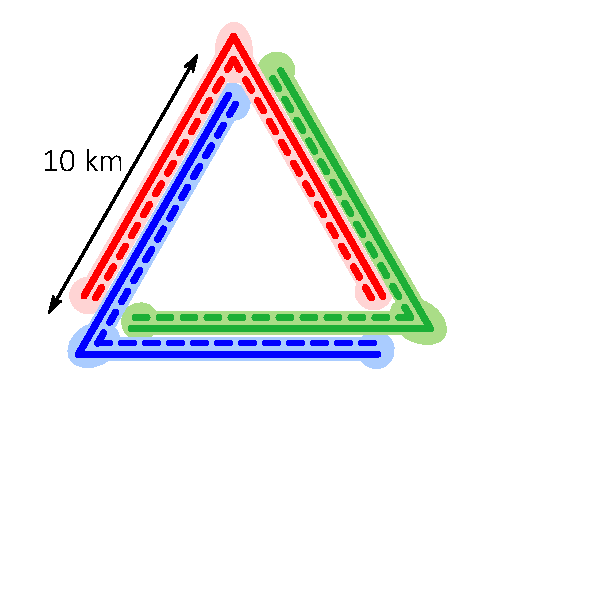
\includegraphics[width=0.35\textwidth]{Figures/ET_simpleB.pdf}
	\caption{The Einstein Telescope will consist of three nested detectors (blue, green, red) in a triangular arrangement. Each detector consists of two interferometers, one optimised for low (solid) and one for high frequency sensitivity (dashed).}
	\label{fig:NestedDetectors}
\end{wrapfigure}

The Einstein Telescope will be a new gravitational wave observatory with a unique design.
A project of this scale must be based on well proven and
experimentally tested technologies. On the other hand, to achieve the sensitivity that the Einstein Telescope
project aims for, it will be necessary to exploit many
state-of-the-art technologies and drive them to their physical limits.
The Einstein Telescope combines the proven concepts from current 
detectors such as LIGO and Virgo with advanced upgrades,
such as cryogenic mirrors, in a infrastructure designed to 
accommodate several technology upgrades over a period of 50 years.

\subsection {Optical Layout and Interferometery}
% Authors A. Freise
\label{Sec:Layout}

The Einstein Telescope aims at providing a significant increase in scientific 
reach through a tenfold improvement of the detector sensitivity in a wide
frequency band, and, in addition, by extending the range of the detector
to lower frequencies. 
The overall improvement can only be achieved by significantly increasing the
length of the detector beyond the size of currently available instruments (i.e.\
3\,km for advanced Virgo and KAGRA, and 4\,km for advanced LIGO) and going to an
underground location, where the seismic noise, and hence the level of gravity
gradient noise, is lower than at the surface. 


By increasing the arm length to 10\,km the influence of unavoidable displacement
noises can be lowered to allow a significant improvement in sensitivity, in
particular at low frequencies. Observing gravitational waves at frequencies well
below the limits of current detectors will also require advanced technologies
such as cryogenic mirrors and active noise cancellation.

The Einstein Telescope is a single-site observatory that will consist of three
nested detectors, arranged in a triangular pattern as shown in 
figure\,~\ref{fig:NestedDetectors}. 
}

The triangle shape, similar to the space-based LISA detector, represents the smallest layout for a single-site observatory that is equally sensitive
to both polarizations of the gravitational wave signal. It also provides
redundancy for continuous data taking during maintenance or upgrades of a single detector, and has the potential for exploiting elaborate data analysis techniques developed for LISA such as null-streams for noise identification and removal.

\subsubsection{A Configuration Covering Multiple-Spectral Bands}

In contrast to all currently existing detectors, each of the three ET detectors will be composed of two interferometers, one specialized for the detection of low-frequency gravitational waves and the other for high-frequency waves. The sensitivity goal for each interferometer is shown 
in figure\,\ref{fig:ET_sensitivity}. This so-called \textit{xylophone}
configuration separates the high laser power required for good high-frequency performance from the cryogenic mirror suspension systems employed for a good low frequency sensitivity into two separate, parallel systems.
In order to achieve a sufficient sensitivity at high frequencies the light power in the arms of the high-frequency interferometer needs to be in the megawatt range. Thermal noise considerations on the other hand require cryogenic optics to reach the sensitivity goal at low frequencies. 
Operating cryogenic optics at a level of several megawatts of light power presents a serious technological challenge that is extremely hard to master. 
Even for the best mirrors that state-of-the-art coating technology can produce, the residual absorption of only about one ppm leads to an absorbed power of several watts at a circulating light power level in the megawatt range. 
The resulting thickness of the suspension fibres, which would be needed to remove the heat, would spoil the performance of the ultra low loss suspension. 
The interferometer dedicated to detecting high-frequency gravitational waves (ET-HF) in the range from about 30\,Hz to 10\,kHz will be operated at room temperature, will use fused silica optics with a diameter of about 60\,cm and a mass of about 200 kg each, will have a light power of about 3\,megawatts in the interferometer arms, and will run with an interferometer configuration optimized for high frequencies (tuned Resonant Sideband Extraction). 
The cryogenic, low-frequency interferometer (ET-LF), operated at a temperature of 10\,K and aimed at the frequency range from 1.5\,Hz to 30\,Hz, will use signal recycling tuned to maximise low-frequency sensitivity, will have a light power of 18\,kW  in the interferometer arms, and silicon mirrors with a diameter of about 45\,cm and a mass of about 200\,kg. 
%\begin{wrapfigure}{r}{0.6\textwidth}
\begin{figure}[ht]
	\centering
		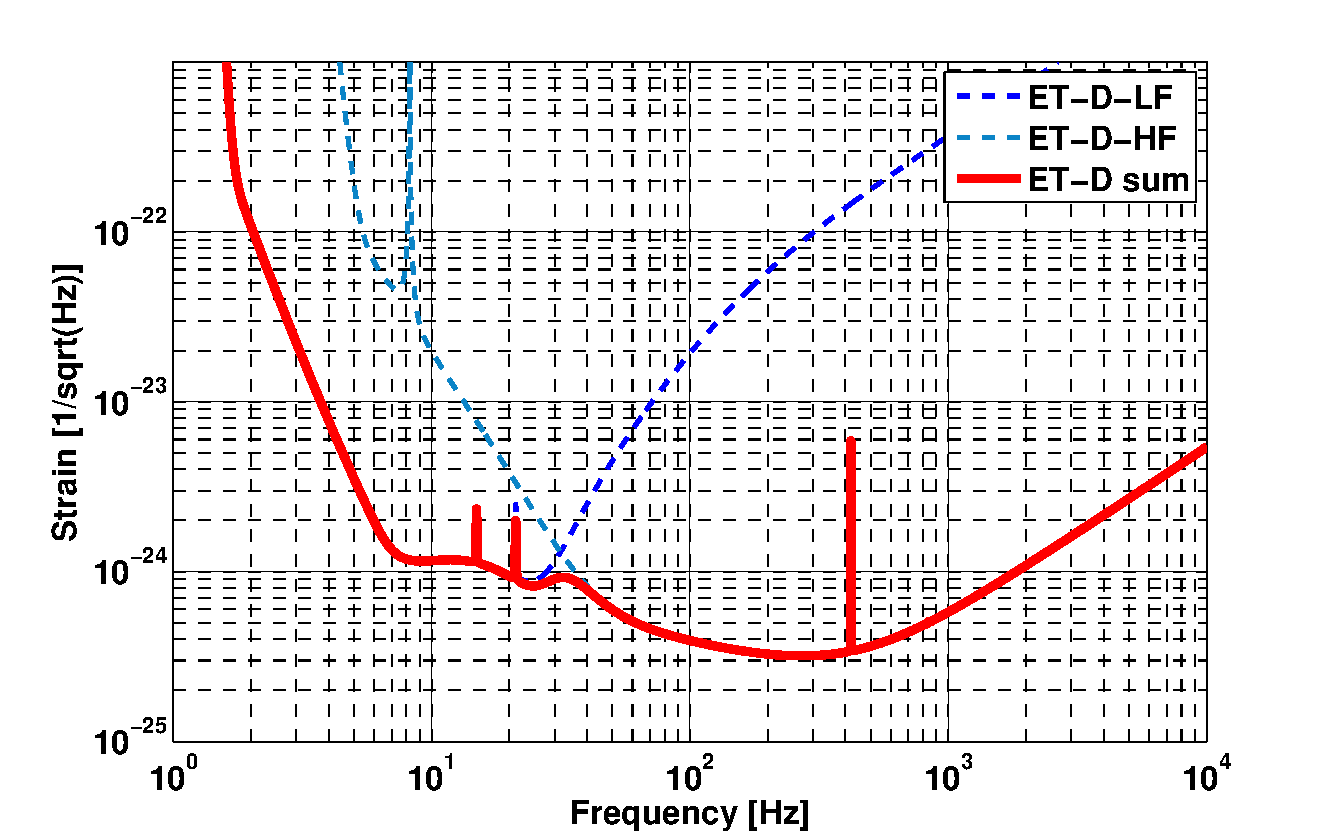
\includegraphics[width=0.6\textwidth]{Figures/ET_D_spectrum.pdf}
	\caption{Sensitivity of the Einstein Telescope. 
	%in the `xylophone' configuration. 
	% comment sth: deleted the last few words as it seemed to suggest that there also are other configurations than the xylophone.
	The sensitivity of the low-frequency cryogenic interferometer is shown in the 
	dashed dark blue curve and the one of the high-frequency room temperature 
	one in a dashed blue-green tone. The resulting total detector sensitivity is
	shown as the solid bright red curve.}
	\label{fig:ET_sensitivity}
%\end{wrapfigure}
\end{figure}

The xylophone configuration addresses two other challenges as well:

\textbf{Control Noises}: Many noise sources limiting the second generation GW detectors at the low frequency end become more challenging with increased optical power: classical radiation pressure forces and torques originating from residual misalignments and beam jitter dominate the dynamics of the interferometer mirrors and hence the local and global control loops. 
The xylophone concept will help ET to achieve its unprecedented low-frequency sensitivity target, by minimising the radiation pressure driven forces on the mirrors of the ET-LF detector.

\textbf{Shot Noise vs Radiation Pressure Noise:} Due to the fact that the shot noise contribution scales inversely with the square root of the optical power, but the photon radiation pressure noise contribution on the other hand scales proportional to the square root of the optical power, it will be hard to obtain the desired bandwidth with a single detector.
The xylophone allows us to optimise quantum noise through operating the high and low frequency interferometers at very different optical powers.

\subsubsection{Core Optics}
%  Author: Jerome
\label{Sec:CoreOptics}
The core optics are the four main mirrors making up the Fabry-Perot arm cavities and are the heart of the ET interferometers.
To ensure the best optics, the three ingredients of a mirror, i.e. substrate,
polishing and coating, must be manufactured using state-of-the-art technology. The temperature at which the mirror is operated has a strong impact on the technological choices to be made.
ET will require larger mirrors than current generation detectors. The large mirror mass will not only reduce radiation pressure effects but will also allow us to use larger sized beam spots on the mirror surfaces for lowering thermal noise  effects. 

\textbf{The mirror substrates} must meet some demanding specifications in terms of optical and mechanical specifications, and should be available in large sizes with surfaces polished to sub-atomic level accuracy. Due to these constraints, only a few specific materials are considered: special grades of fused silica for room temperature interferometer and ultra-pure silicon for cryogenic temperatures.
% comment sth: I added some adjectives to indicate that the reader understands already here that it is not any fused silica or any silicon we can use, but within these materials we still have very specific requirements like Suprasil 3001 or floatzone/magnetic CZ silicon.

Fused silica
is the substrate of choice for all the current room temperature interferometers.
Due to its use for first and second generation gravitational wave detectors, this material has been extensively characterised at room temperature.
Moreover the polishing and coating technologies are now highly developed for this material.
Serving as a pathfinder for ET, the upgrade of Advanced Virgo, called Advanced Virgo+ will use fused silica test masses with a diameter of  55\,cm and a weight of 100\,kg. 

Silicon is the preferred candidate material for the test masses for the cryogenic ET low-frequency interferometers. 
Unlike fused silica, silicon is not transparent at a laser wavelength of 1064\,nm and so the operating wavelength of the LF interferometers has to be shifted to 1550\,nm. 
In contrast to fused silica, silicon has excellent mechanical and thermal properties at cryogenic temperatures and is easily available in relatively high quality due to the large market of the semiconductor industry.
%The coefficient of thermal expansion is zero at two special
%temperatures around 18~K and 125~K \cite{lyon1977siliconexpansion}. At these
%temperatures the contribution of thermo-elastic noise will therefore vanish. 
%
%It was
%experimentally shown that silicon bulk samples can reach mechanical losses as
%low as $1 \times 10^{-9}$ at 10~K. \cite{mcguigan1978siliconQ}.
The maximum available diameter and purity of silicon depends on the fabrication
process. The two main growing processes for single crystal silicon used by the
semiconductor industry are the Czochralski (CZ) and the Float Zone (FZ) methods.
CZ silicon is grown from a silicon melt in a fused silica crucible, resulting in relatively large samples with reasonable purity. 
%The most dominant impurities
%in undoped CZ-grown silicon are carbon (typically 10$^{-18}$ cm$^{-3}$) and
%oxygen (typically up to 10$^{-19}$ cm$^{-3}$). 
In comparison, FZ silicon also contains impurities but in much smaller concentrations (up to 10$^{-3}$ times smaller). 
Using the CZ growth technique, silicon ingots up to 45~cm of diameter can be produced though 30\,cm is still the dominant wafer diameter in the semiconductor industry. For FZ silicon the diameter is currently limited to 20\,cm.
In the recent years the optical properties of silicon have been thouroughly characterised. According to the latest measurements, the magnetic Czochralski (mCz) growth technique is the most suitable approach for ET as it can combine large diameter ingots (45\,cm diameter) with very low impurities and absorption at the 20\,ppm/cm level. These level of absorption are promising but further developments are required, and the effects of residual birefringence intrinsic to crystalline materials have to be evaluated.
%has been achieved on one sample.
A backup substrate choice could be sapphire as a candidate material for ET-LF. Sapphire is already used in the Japanese cryogenic interferometer KAGRA, though much smaller in size than what is required for ET, and hence extensive experience has been acquired on operating those mirrors  in cold conditions.% \cite{Akutsu_2019}. 
Like for silicon, large sapphire boules with excellent optical properties still have to be demonstrated.

\textbf{Polishing of the surfaces} of fused silica substrates is well mastered
thanks to the current generation of room temperature interferometers as well as EUV
lithography optics and hence presents minimal risks. For the Einstein Telescope
main mirrors, the already-demonstrated surface quality such as surface
height errors below 0.3\,nm RMS for low spatial frequencies (flatness) and below\,0.1 nm
RMS for the roughness (smaller defects) will be enough, albeit it must be
achieved on a larger area since the ET mirrors will be bigger.

Polishing of silicon does not carry any difficulties as this substrate material is heavily used for X-ray mirrors, but demonstrator meeting all the ET polishing specifications will have to be produced. Experiences from polishing companies indicate that silicon could be polished the same way as fused silica and similar surface figure accuracy and roughness can be achieved (using also ion beam figuring to reach sub-nanometer flatness). The very low roughness is more challenging but 0.2\,nm RMS could be achieved and is acceptable for ET. 
%Andreas: The number comes from Jerome
%\todo[inline]{Not sure where this number comes from and about the fact that excellent micro-roughness is harder to achieve. I do not think that we would be happy with 0.2nm micro roughness even now for advanced optics... "roughness" per se is ill defined without saying which spatial frequencies we are talking about. Currently achievable values for surface figure errors are limited by the measurement capabilities and range in the 50 pm rms range.}

\textbf{Thin optical coatings}, a few microns in thickness, must be added to the surfaces of the mirrors to make them highly reflective for the used laser wavelength. 
Since the thermal noise from these coatings will limit the sensitivity of current room-temperature detectors at their most sensitive frequencies, it is essential to reduce coating thermal noise to achieve the ET design sensitivity.
To meet the goal of a factor of 25 improvement in sensitivity over Advanced LIGO design sensitivity at 10 Hz, ET-LF requires a reduction in coating displacement thermal noise by at least a factor of 10 with respect to Advanced LIGO.
Some of this improvement can be obtained from operating at low temperature and through the use of larger laser beam spots on the mirrors.
The target for ET-HF is a factor of 3.2 reduction in coating thermal noise
amplitude spectral density (ASD)
at 100 Hz compared to Advanced LIGO design sensitivity. Accounting for the slightly
larger laser beam in ET-HF, this sets a requirement of a reduction in ASD by a
factor of 2.7 from the coating materials. If we assume all coating properties
except the mechanical loss remain identical, then a reduction in mechanical loss
by a factor of 7.1 with respect to the Advanced LIGO coatings would be required.

Significant progress has been made towards development of coatings suitable for low temperatures in ET-LF. There are several highly-promising routes to meeting the coating thermal noise and optical absorption requirements. 
However, further studies are required optimising the trade-off between coating absorption requirements, suspension thermal noise, ultimate mirror temperature and substrate thermoelastic noise.
% – and it seems likely that lower absorption than 5 ppm may be required.
Achieving significant reductions in coating thermal noise at room temperature
may be more challenging than at low temperature. Work in this area is ongoing,
both for ET and for upgrades to the Advanced LIGO and Advanced Virgo detectors.
%, and there are several promising avenues which are currently being investigated. 

\subsubsection{Michelson interferometer}

Each individual interferometer has a classical dual-recycled Michelson topology with arm cavities. This is a mature technique, well tested by  
second-generation detectors, Advanced LIGO and Advanced Virgo. More elaborate topologies like Sagnac interferometers fit equally well into the planned infrastructure but are not considered for the initial installation, as they have not yet reached the required level of maturity.

Each of the ET interferometers will require a novel high power laser system with
low intrinsic noise called the high power laser (HPL) in the following. 
The ET-HF HPL has to operate in a single-frequency continuous-wave (cw) mode at a wavelength of 1064\,nm and needs to deliver 700\,W in a linear polarized fundamental spatial HG$_{00}$ mode. With the assumption of roughly 30\% loss in the injection path this leaves 500\,W at the input of the main interferometer. The higher order mode content of this laser should be below 10\% and the polarization purity at least 1/10. 
The ET-LF HPL needs to operate in a single-frequency continuous-wave (cw) mode at a wavelength of approximately 1550\,nm with similar spatial and polarization purities as the ET-HP HPL. This different wavelength for ET-LF follows from the material choice for the test masses.
A laser power of 5\,W is required to allow for 3\,W to be injected into the main interferometer. Both laser systems have to achieve demanding noise requirements for all frequencies in the observation band:
a frequency noise in the $10\,\mathrm{mHz} / \sqrt{\mathrm{Hz}}$, relative lateral
and angular beam fluctuations in the $10^{-6} / \sqrt{\mathrm{Hz}}$ range
and a laser power stability of roughly RPN $= 3\!\times\!10^{-10} /
\sqrt{\mathrm{Hz}}$. These requirements appear to be feasible using current approaches to stabilization.

Advanced detectors have recently been upgraded with \textit{squeezed light} which generates correlations between the phase and the amplitude quadratures. In the shot noise  dominated frequency range squeezed light is used which shows lower phase fluctuations (at the cost of the amplitude fluctuations) in comparison to classical  laser light in the interferometer arms. In the low-frequency, radiation pressure dominated range the fluctuations need to be lowered in the amplitude quadrature. 
%This goal can be 
Providing the right spectral dependence of the so-called \textit{squeezing angle} can be  achieved by reflecting squeezed light off a filter cavity. 
For the ET we assume 15\,dB initial squeezing level at the squeezing source and an effective squeezing level of 10\,dB to be 
available (equivalent in shot noise reduction to a laser power increase of a factor
of 10). 

The squeezing level, and with it the sensitivity improvement that can be reached, 
depends on the optical losses in the squeezer, the filtering optics, the interferometer, 
and all optical devices on the way to the photodetector, including the photodetector 
efficiency itself. It will therefore be essential 
to keep the optical losses as low as possible. 
These levels of squeezing, and maintaining the low losses required to preserve the squeezing, will require technology development.
%Optical losses of 75\,ppm per round 
%trip are currently achievable with state-of-the-art techniques and are used as a 
%conservative estimate for the filter cavities.


\subsection{Seismic Isolation and Suspension}
% Authors: Giovanni Losurdo, Giles Hammond, Conor Mow-Lowry
\label{Sec:SASandSUS}
%\subsection{Seismic Isolation System}


Seismic isolation refers to the stage(s) of isolation systems closest to the ground. It fulfills two main
functions: to suppress the seismic noise below the sensitivity requirements in the detection frequency range
(for ET at frequencies larger than 1-2\,Hz); and to reduce the RMS input motion to the suspension systems,
particularly at the suspension resonances and the micro-seismic peak(s). It also provides large-scale and
slow position control of the test-masses.

The baseline for ET, originally defined in the 2011 ET conceptual design report, consists in using a longer Virgo-style
Superattenuator. The increased length (17\,m) reduces the normal mode frequencies, pushing
the seismic wall down to $\sim 2$\,Hz. The main advantage for such a choice is that it employs a design
thoroughly tested during many years of operation in Virgo and it requires relatively little R\&D to be
adapted to ET. It therefore represents a safe pathway towards a 3G configuration.

A possible alternative to be investigated via a dedicated R\&D program is the
coupling of a Superattenuator to an inertial platform controlled in all 6
degrees of freedom. 
This configuration would make use of a combination
of technologies and expertise developed in the GW field in the last decade. The
inertial platform would support the Superattenuator, an approach that was
envisaged for use in Virgo. The Superattenuators are supported on a rigid
platform resting on 3 elastic feet that can be actuated by piezo actuators in
order to actively control of the ground tilt. The ET design would extend this concept to also improve horizontal performance.
An advantage of this alternate could be relaxed requirements on the physical infrastructure, providing an advantageous cost and risk trade.

%Such an approach could in principle allow to shorten the Superattenuator height and, consequently, the height of the caverns.
%Comment by stefan: While I completely agree with this statement, I am not sure if this sentence helps our ESFRI application and hence I would advocate to remove the previous sentence for now.)


%\subsection{Test Mass Suspension Systems}
\subsubsection{Thermal noise of the mirror suspensions}
The main requirements of a gravitational wave mirror suspension are to reduce seismic noise input from the ground and to provide a mechanism to steer the mirror via electromagnetic/electrostatic forces for alignment and control. This must all be done while minimising the thermal noise arising from the suspension. Suspension thermal noise arises due to mechanical dissipation in the materials which make up the suspension (Brownian noise) or through thermoelastic noise, the coupling of statistical temperature fluctuations through the thermo-mechanical properties of the suspension materials such as the thermal expansion coefficient and the Young's modulus. \\
{\bfseries High Frequency Suspension}: The current room temperature
interferometers (Advanced LIGO, Advanced Virgo, GEO) utilise fused silica as a material to
suspend the test masses. The suspensions were initially pioneered in GEO
around 1990-2000 (5.6~kg optics),  upscaled for use in Advanced LIGO and Advanced Virgo (both
40~kg optics) between 2000-2012, with installation occurring from 2015 onwards.
Fused silica is the material of choice as it can be pulled into long thin
fibres, can be welded to form monolithic structures, has extremely low internal
friction,  and has a breaking strength in excess of 4~GPa. The ET-HF
suspension mirror mass will be increased to 150~kg - 200~kg to provide lower
suspension thermal noise and also reduction of radiation pressure noise. There
is a mature technology in place to deliver the technology for a room temperature suspension, building on many years of heritage and proven technology in the field. The Heraeus Suprasil family of synthetic glasses will be utilised, and initial work has shown that fibres of suitable geometry can be pulled and
welded. While the fused silica solution is already well developed, there needs to
be work devoted towards the demonstration of a full scale ET HF prototype. Key
areas of future R\&D include
the testing of a full scale prototype suspension with fused silica fibres with
operating stresses of around 1 - 1.5~GPa;
activities to prove the stress-corrosion properties of fused silica, and the
techniques required to bond/attach the ear/fibres to the test mass; the
demonstration of sensors and actuators with sufficient sensitivity 
%and control authority 
for suspension local control and damping; and the demonstration of mitigating
excess charges in electrostatic actuation.\\
{\bfseries Low Frequency Suspension}: In addition to providing a low seismic/thermal noise platform, the ET Low Frequency suspension also has to fulfill a second crucial duty - to extract the thermal load that is put into the optical component by the laser beam ($\simeq 10 $mW). The materials of choice are crystalline materials that have a very high thermal conductivity at low temperatures and also display low mechanical loss. In particular, both silicon and sapphire are excellent materials in the temperature region of interest (typically below 20\,K). Sapphire has a higher thermal conductivity than silicon below 20\,K. Sapphire fibres for heat extraction have been investigated in detail by Japanese groups for KAGRA. At low temperatures the mechanical loss of the suspension, which defines the thermal noise performance, is a key driver for the suspension design. Heavy test masses will be utilised, with the addition of low temperature to provide enhanced thermal noise performance. Thermoelastic noise drops away sharply with decreasing temperature, and indeed for silicon is zero around 120~K and as $T<20$~K. While sapphire is the baseline for KAGRA, the need for large and heavy test masses (150~kg - 200~kg) highlights silicon as a preferred material for ET-LF.  Silicon suspension elements are currently under investigation in the form of fibres and ribbon-like geometries. Fabrication techniques include (i) Laser Heated Pedestal Growth, (ii) micro pull down and (iii) etching from wafers. R\&D activities are needed on several aspects of the low frequency suspension:
\begin{itemize}
\item fibre fabrication techniques, to develop long thin silicon or sapphire fibres, and to join the suspension elements to the ears and test masses;
\item detailed FEA modeling of the final stage suspension, in order to estimate the effects of real fibre geometries on the thermal noise performance;
\item inertial sensors and actuators, operating at cryogenic temperature, with high sensitivity and large bandwidth; 
\item prototyping the lower stage suspension, including a fast turnaround tabletop systems and small scale prototypes of 10\,m arm length with payload in the 1\,kg to 10\,kg range.%Gianluca: this last point is not clear. It means that we need to build a 10m arm ifo?
\end{itemize}

\subsection{Vacuum System}
% author G.Gemme
\label{Sec:Vacuum}
In laser interferometers for GW detection the instrument has to be kept under High-Vacuum or Ultra-High-Vacuum (HV, UHV) for several reasons: 
\begin{itemize}
\item reduce the noise due to residual gas fluctuations along the beam path to an acceptable level; \item isolate test masses and other optical elements from acoustic noise; 
\item reduce test mass motion excitation due to residual gas fluctuations;
\item reduce friction losses in the mirror suspensions  contribute to thermal isolation of test masses and of their support structures; 
\item contribute to preserve the cleanliness of optical elements. 
\end{itemize}
The power spectral density of gas-induced fluctuations in the optical path length has been calculated choosing conservative beam shape parameters and taking a safety factor of at least $10$ with respect to the pressure producing a phase noise at the limit of the best sensitivity for the ultimate detector envisioned for ET.
The residual gas composition will be dominated by hydrogen with presence of water and other gases; we will keep the total residual pressure at about $10^{-10}$~mbar, corresponding to a noise level below $10^{-25}$~Hz$^{-1/2}$.
The vacuum system will be extremely clean from heavy organic molecules, both to limit the phase noise and to prevent pollution of the optical components. Hydrocarbon partial pressure shall be at the level of $10^{-14}$~mbar.

The technologies that were developed and employed in the existing gravitational wave observatories have been shown to meet the stringent requirements of vacuum integrity, very low hydrogen and heavy molecule outgassing, minimal particulate generation, low vibration, and appropriate stray light optical absorbance for successful operation. However, straightforward extrapolation of the costs for extending the interferometer vacuum beam enclosures from the current lengths of 3-4~km/arm to $\sim10$~km/arm indicates the need for investigation of a range of technologies and materials that could significantly lower the final cost, facilitate construction and increase the life-cycle operation of vacuum systems for next generation observatories. 

\begin{comment}

The baseline choice for the material of the vacuum enclosure is stainless steel (304L), based on the experience of first-generation installations. Two alternative options are a low carbon, mild steel alloy and aluminum that could both offer significant cost savings. Regarding these options, some open issues need to be studied and clarified. These include choice of the mild steel alloy, potential surface treatments or coatings for the mild and stainless steel and the aluminum alloy, and the cost of incorporating the many transition elements (flanging and expansion joints) if aluminum is chosen as the base vessel material.

In order to minimize the cost of in-situ bake out systems for removal of adsorbed water following the initial or subsequent exposure to air, a number of potential surface coatings are being investigated for stainless and mild steels including TiC, diamond-like carbon (DLC), amorphous Silicon (a-Si) and a class of conversion coatings such as magnetite (Fe$_3$O$_4$) that could be applied during the mill processing of the steel (so-called conversion coatings). A number of characteristics of these coatings were identified for further study before their cost effectiveness could be quantified including additional H$_2$O adsorption studies, coating deposition costs at scale, film toughness, particulate generation, interference with vessel welding, and optical characteristics.

Viable first order pumping schemes are being considered. Specific pump-down routines were identified from atmospheric pressure to UHV using pumps that would minimize or eliminate hydrocarbon or particulate contamination. The continued use of large area liquid nitrogen panels is recommended based on the high-water pumping speed and satisfactory performance in current generation systems. UHV performance can be maintained with periodically spaced getter pumps and ion pumps. The availability of the new getter alloy from SAES (ZAO) is particular useful for this application because of its large pumping speed and capacity for H$_2$O and H$_2$. In addition, conventional titanium sublimation pumps (TSP) are not ruled out for consideration.

The use of clean, ultra-dry (ppb water), warm gas purging systems could significantly affect the need for in-situ bake-out systems for removal of adsorbed water following the initial or subsequent pump-downs from atmospheric pressure. The incorporation for such systems for the first-generation gravitational wave observatories can significantly shorten downtime in the event of a loss-of-vacuum incident.

Finally, the value of partnerships with industrial contractors with relevant expertise was demonstrated by the successful design, installation and operation of current installations. Such partnerships can be valuable in the pre-competitive phase to test the viability of the proposed concepts and they are certainly valuable in the final design and early constructions phases to test prototypes of full vessel segments.

\end{comment}

\section{Cryogenics}
%author F. Ricci
\label{Sec:Cryogenics}

The  low-frequency ET detector test masses will be cooled below 20\,K to reduce thermal noise, which represents a limit to the low-frequency sensitivity for the second generation of detectors.  The payload, i.e. the last stage of the test mass suspension, will include a mass used to steer the mirror, called marionette, where the thin wires used to suspend a massive silicon (or sapphire) mirror are attached. The payload mass will be about one ton and it will be cooled in a dedicated cryostat, which will include two radiation shields at 8\,K and 80\,K.  
The entire payload and cryostat will be hosted in the lower part of the vacuum tower hosting the long Superattenuator
% this tower base will be a cryostat with two radiation shields.
 The need to preserve the high mechanical quality factor of the mirror and the ultra-high  quality of the optics imposes the requirement to keep the mirror at low temperature in vacuum avoiding any mechanical contact or exchange gas. %even relying to a molecular conduction process via a residual helium gas pressure left on purpose in the inner vacuum chamber of the cryostat. 
 This imposes stringent dimensional requirements on the mirror suspension wires, that represent the only conductive path to transmit the refrigeration power and keep the optical element in thermal equilibrium. % when  kilowatts of light power are impinging on it, will be dimensioned on the base of this cryogenic constraint. 
In order to avoid the vibration noise generated by the cooling system, a cold-box will be connected to a marionette via extremely soft heat-links of high thermal conductivity (similar links have been developed already in KAGRA). The cold-box will host superfluid $^4$He provided by refrigeration plants installed on the surface in correspondence of each vertex of the detector, and connected with %so that the cryogenic fluids are sent to
the underground cryostat by long transfer lines. %, as done for LHC at CERN. 
Using similar thermal links we plan to cool the 8\,K shield, while for the outer shield the use of the cold He gas evaporated from the cold-boxes should be sufficient to guarantee thermal equilibrium around 80-100\,K.
This last shield will be wrapped by super-insulation sheets of special fabrication, as the standard super-insulation material can be a source of potential pollution of the inner vacuum where the mirror is hosted. 
Moreover, in order to reduce the thermal radiation from the beam duct into the cold mirror, liquid helium cryotraps, tens of meters long, will be installed along the vacuum tubes and appropriate low-emissivity coatings will be deposited on their inner walls. 

\section{Site and Infrastructure}
\label{chap:Site}

\subsection{Site requirements and characterisation}
% author J.Harms
\label{SiteReq}
The achievable detector sensitivity and duty cycle, infrastructure lifetime, and its construction cost depend strongly on the characteristics of the ET site. This concerns underground parameters such as rock quality, groundwater, and site stability, but also surface parameters such as remoteness of the site, accessibility, and connection to existing infrastructure including public utility. In addition, socio-economic criteria must be considered for a big infrastructure like the Einstein Telescope, and it is important to understand and respect the interest of the local population. 

The achievable detector sensitivity, duty cycle and infrastructure lifetime are of prime interest to the science community. The impact of environmental noise on detector sensitivity is discussed in Section \ref{sec:envnoise}. The duty cycle of a detector also depends on its environment since regional earthquakes, but potentially also major storms, railroad traffic and other anthropogenic sources can produce enough ground motion to make a continuous operation of the detector challenging or impossible. In terms of ET's immediate science return, site parameters affecting the sensitivity of the detector are most important, but infrastructure lifetime determines how many cycles of major detector upgrades leading to sensitivity improvements one will be able to realize, which means that infrastructure lifetime plays an equally important role. 

The lifetime of an underground infrastructure is above all influenced by groundwater conditions (hydrogeology) and geological stability. Water inflow into tunnels requires water-handling systems, which might act as underground sources of seismic noise. Water that is being moved to the surface typically must be considered waste and pass through a water-treatment plant. The presence of water in the tunnels increases the humidity of the tunnel air, which drives atmospheric corrosion potentially accelerated by the presence of certain elements in groundwater such as chloride, and of microbes, e.g., sulfate-reducing bacteria, leading to microbially induced corrosion. Air humidity is controlled by ventilation systems that may also act as sources of underground seismic noise. With time, drainage systems to prevent water inflow can deteriorate leading to water leaks and tunnel lining deformation, which means that monitoring and maintenance are necessary in aged tunnels. 

Geological conditions determine the site stability. The most stringent requirements on differential motion across the tunnels does not come from the tunnel construction itself, but from the hosted detector infrastructure. The vacuum pipe will be mounted as a series of modules welded at their interfaces. Stress on the welding lips needs to remain small over the infrastructure lifetime. For example, across the 15\,m modules used in the Virgo detector, only a few millimeters of integrated differential displacement is tolerable. Another requirement comes from the positioning of the optical axis inside the vacuum pipe, which means that one needs to impose a maximum differential displacement across the full tunnel length as well. Drilling of the tunnel through active shear zones must therefore be avoided, and subsidence should be limited by driving the excavation through high-quality rock, or by employing hydraulic pipe-alignment systems like in Virgo.

Characterization of the site will happen in two steps. A preliminary survey of both candidate sites is required for site selection, relying mostly on surface measurements and analyses, and on a collection of already available site data. A few boreholes are mandatory to have at least some information about groundwater conditions, local geology, and underground seismic spectra. This information will be used to obtain first construction-cost estimates and to predict eventual complications in tunnel construction and maintenance. Characterization of environmental noise over at least a year is important to make accurate noise predictions for ET. Generally, the impact of the candidate sites' environments on ET sensitivity and operation needs to be assessed and evaluated. Solutions need to be found for waste removal (rock from excavation and tunnel water), and local support needs to be secured for realizing the ET infrastructure and for preserving the site quality. Once the site is chosen, extensive borehole studies of the future ET site will be necessary for construction planning and for a detailed cost estimate. 

\subsection {Newtonian Noise and other Environmental Noise}
\label{sec:envnoise}
% Author:  Jan Harms
Several environmental factors can influence the sensitivity of a gravitational-wave detector. Most importantly, seismic fields produce ground vibration that needs to be filtered out by a seismic isolation system for the suspended test masses. Seismic fields also lead to perturbations of the gravity field, which produces another random force on the test masses. Detector noise produced by terrestrial gravity fluctuations is also known as Newtonian noise to distinguish it from the effect of gravitational waves, which are described by general relativity. Similarly, atmospheric gravity fluctuations from acoustic, temperature and humidity fields are sources of Newtonian noise. Acoustic fields also act as sources of vibration of detector structure together with seismic fields. Electromagnetic fluctuations can produce detector noise by coupling with magnetic components of the detector, or by inducing noise at connectors and in cables acting as antennas. Finally, cosmic rays might cause test-mass charging, which then leads to excess noise by altering the dynamics and thus impeding the performance of the seismic isolation system. 

None of these environmental factors can be neglected ad hoc in ET. It is likely that test-mass charging by cosmic rays will not play a role in ET, and possibly is not the dominant charging mechanism in surface detectors either, since the underground environment acts as a shield against cosmic rays. Newtonian noise from atmospheric fields is mitigated by constructing ET several hundred meters underground leaving only minor (but likely significant) contributions to Newtonian noise from acoustic fields in the caverns. The seismic isolation system will be designed with the goal to provide sufficient seismic isolation without depending significantly on properties of the seismic field. Electromagnetic fluctuations, either being produced by the detector electronics or associated with Schumann resonances, depend weakly on the site where the detector will be built leaving seismic Newtonian noise as the main site-selection criterion with respect to environmental noise. It is crucial though that the underground environment will not be perturbed by detector infrastructure like the cryogenic system, water pumps, ventilation, and other machinery required to operate the detector. Experience with the Japanese underground detector KAGRA will help to optimize the ET infrastructure design to avoid excess noise.

Only some contributions to seismic Newtonian noise decrease with increasing detector depth. The contributions suppressed underground are mostly associated with seismic surface waves. Contributions from so-called body waves, i.e., seismic waves able to propagate in all directions through Earth, depend weakly on detector depth. In other words, the body-wave contribution sets a lower limit to seismic Newtonian noise, which is reached when the detector is so deep that body waves dominate the local seismic field and surface contributions can be neglected. Underground levels of seismic displacement are therefore a strong site-selection criterion. Newtonian noise in ET from seismic surface waves can also be significant, even many 100\,m underground, depending on seismic speeds. However, while there is no known technology that could mitigate effectively Newtonian noise from body waves, surface waves could be easily monitored by seismometer arrays and the seismic data be used to subtract efficiently the associated Newtonian noise from ET data if necessary. 

\subsection{Tunnels and Caverns}
% author G.Losurdo, A Paoli
\label{Sec:TunnelsCaverns} 

The design of the underground infrastructure is based on a trade-off between the
cost of the realization and the fulfillment of several scientific requirements,
such as, the capability of hosting the 6 interferometers, the availability of free space, safety, 
etc. The main elements are: the tunnels, the caverns, the access routes. Important
works are also needed on surface, with the realization of buildings and roads.

The underground scheme consists of an equilateral triangle of an approximate side length of 11\,km. The access is granted in the form of an inclined access tunnel or a vertical shaft, which connects the caverns at the intersection points with the surface.
The access tunnels/shafts are the main points of access during construction and operation. Several caverns of various geometry are situated in the vicinity of the intersection points. An additionally lined borehole/service tunnel offside the crucial and vibrational sensitive cavern structure is foreseen for water management during operation.

\paragraph{Tunnels}

%The three 10\,km tunnels will be excavated by TBMs, producing an inner free
%diameter of 6.5\,m.  
Due to the length of the tunnels, a mechanised excavation method utilising Tunnel Boring Machines (TBMs) is considered for the design stage. It is envisaged to excavate the whole length of the tunnel in one stretch without further points of intermediate access.
%\todo{Add a mentioning of mini-caverns every now and then (say 1\,km) for gate valves and pumping stations}
The inner diameter will be 6.5\,m, needed to host 4 vacuum pipes, which must be straight to several\,cm (and not follow Earth's curvature). The outer diameter could vary in a range between 7.3\,m and 8.4\,m depending on the type of TBM excavation (shielded or open TBM) and consequently by the kind of lining of the excavated tunnel (segmental pre-cast or shotcrete lining). 
The concept of the shielded TBM type considers a continuous mining process with parallel installation of a segmental lining, which takes over the support of the rock mass. A single-layer segmental lining with all-rounded preformed elastomer gaskets would be used to control water inflow to the tunnel. Thus the thickness of the reinforced concrete segments is at least 30\,cm.
Contrary to a shielded TBM, the open TBM is based on applying shotcrete, steel ribs and rock bolts. As part of the excavation concept, rock mass grouting is considered, to decrease the overall inflow of groundwater to the tunnel, since the shotcrete support is more prone to water inflow.
The overall thickness of the shotcrete support layers is also of the order of 30\,cm thick consisting of two layers. Regardless of the straight direction demanded for the subsequent installation of the vacuum pipes in the tunnels, the TBM excavation implies an inherent meandering of the tunnel axis as a reaction to heterogeneous geological conditions while driving. 
%A predefined additional over-excavation should be considered, to avoid interference of the clearance profile of the tunnel with needed space the steel tubes, which is of the order of 10 cm for the open TBM, while 65 cm for the shielded one [TBD].
 \begin{figure}[tbh]
	\centering
		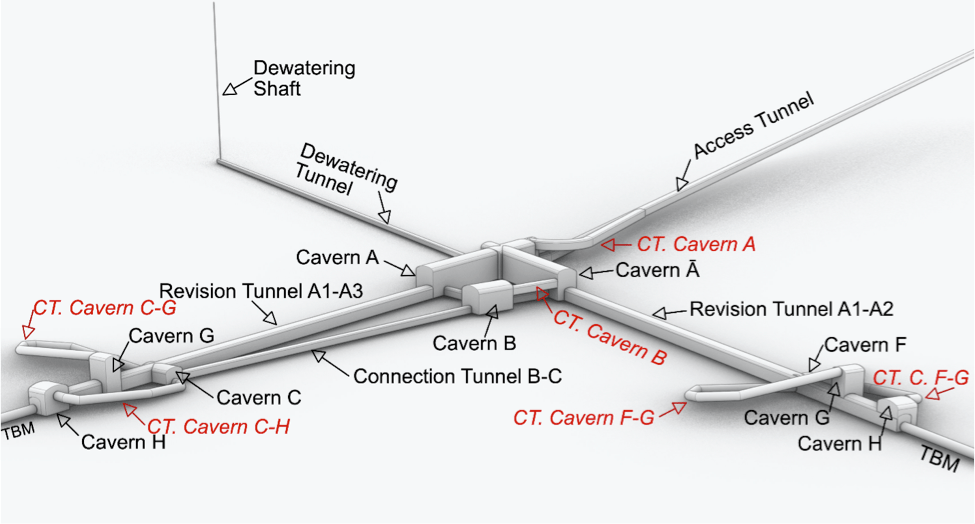
\includegraphics[width=0.9\textwidth]{Figures/ET_caverns.png}
	\caption{Sketch of the cavern layout of the ET in one corner of the
	triangle. 
	All labels in red refer to constructionally required galleries or tunnels.
	\label{fig:ET_caverns}}
\end{figure}

\paragraph{Caverns}

For each vertex of the triangle layout, “Cavern A” (see Figure~\ref{fig:ET_caverns}) indicates the main cavern structure of the underground laboratory and is formed by an intersection of two caverns with an identical layout at an angle of 60°, with lengths of about 190 m and 160 m.
The smaller cavern branch (Cross-Cavern A) includes a prolongation tunnel about 1 km long, hosting the Filter Cavity. 
Two identical connecting 465\,m long tunnels run in the prolongation of the branches of “Cavern A”. Each connecting tunnel contains a series of three caverns (Cavern C-F/G/H) at the transition to the TBM tunnel. The three caverns have a spacing of 35\,m in between them. 
%The distance between the caverns is mainly required from an operational point of view but will be also deemed to be adequate from a geomechanical perspective.
The “Cavern B” is located within the bisection line of the two branches of the “connecting tunnels”. It is linked to the two branches of the “Cavern A” and carries an additional connection tunnel to the Cavern C. 
%The Cavern C is situated 316 m offside the Cavern B and the connection tunnel will host the filter cavity reserved to the “calibration” of the interferometer [TBD].
The caverns and the connecting tunnel are of various shapes and will be excavated by drill and blast. The design foresees a horseshoe-shaped design of all cavern, tunnels and galleries. The shape of these caverns and tunnels might be redesigned to fit the geomechanical requirements.

\paragraph{Access}
    
The underground infrastructure can be accessed by elongated inclined tunnel ramps or large vertical shafts. The best option may strongly depend on the geography, geology and surface land use and will therefore be finalized after the choice of the site. 

Three construction methods are available: access by inclined elongated ramp; access by inclined helical ramp; access by vertical shaft.
An “inclined elongated ramp” equally to an “inclined helical ramp” connects the
surface with the cavern structure situated a few 100\,m below the ground surface. The length of the access tunnel is considered based an overall slope of max. 10\%. It is not required to drive the access tunnel as a straight line, any combination of the straight and curved section is possible.
The clearance profile of any inclined tunnel shall support all aspects of construction, mucking and ventilation. 

Daylighting shafts are the shortest connection of the surface to the underground structure. The vertical shaft is considered as the single line of access during construction and operation. Nevertheless, for the long-term service, changes to the shaft hauling system are necessary to comply with the demands of the laboratory.

The decision on the best type of access depends on a combination of ecological, logistical (connecting roads), geological/hydro-geological, safety and monetary aspects. 
Due to further site-dependent impact factors, currently only the monetary
aspects of the access have been analysed. 
%In any way from a constructional point of
%view, the inclined access tunnel is the most conservative layout. 
Both types of access can be accomplished with standard tunnelling equipment.
The shaft solution implies the utilisation of specialised equipment for shaft lowering, while the inclined access tunnel can be excavated with standard tunnelling equipment, as foreseen in any way for the excavation of the underground caverns.

\subsection{Roads and buildings}
% author G.Losurdo, A Paoli
\label{Sec:RoadsBuildings}

The construction of the ET facility will include all the surface technical and general buildings needed for the construction and operation of the research centre.
The surface buildings will be located mainly in correspondence of the access points to the underground infrastructure and consist of the following list, with the corresponding estimated volume at this stage of the project: laboratories for the construction and the installation, warehouses, clean rooms, mechanical and electrical workshops, control buildings, office buildings, technical buildings for plants, visitor centre, access buildings.
%TODO  [Volume per category to be added].


\section{Computing Infrastructure}
\label{chap:GlobalComputingInfrastructure}
As with most large experiments, the scale of ET computational challenges is such that the computing infrastructure architecture cannot be solely based on local resources. 
We expect that most of ET computing will be done off-site in external computing centres, also including much of the low-latency searches. 
So, the on-site computing infrastructure will be limited to what is needed for detector control, data buffering, preparation and transfer, unless special needs will be discovered (for example, the need for sizable AI clusters to manage some aspect of detector control such as alignement optimization). The physics community at large has a long experience in designing, building and managing global-scale computing infrastructures that can be exploited to cater to such needs; the main GW peculiarity here is the need to generate low-latency alerts
for the wider astronomical community.  

\subsection[Computing challenges and strategies]{Computing challenges and strategies}
\label{sec:Computing challenges and strategies}
ET will not, even by today's standards, generate a huge data volume with respect to the 1\,PB of data per year produced by a 2G interferometer; it is the quantity of valuable scientific information hidden in the data that will grow, and with it the amount of computational power needed to extract it.  Factoring in the expected technological developments in computing hardware (Moore's law is starting to fail for CPU performance, whereas its network capacity equivalent is not), it turns out that data management will most likely not be an outstanding issue; computing power itself, however, will be challenging, particularly for Compact Binary Coalescence matched-filter searches and parameter estimation. The better sensitivity implies a larger parameter space to explore, so much larger template libraries have to be used for matched-filter searches;  the computing power needed for parameter estimation of course scales with the expected event rate. 


Even not taking into account complications such as the analysis of day-long
signal candidates, for which the detector moves with respect to the source, a naive extrapolation from current activities gives an increase of \emph{at least} three orders of magnitude in computing power from 2G to 3G data. This is clearly out of reach, and a number of mitigation actions need to be planned (exactly like what is being done today in the HEP community for High-Luminosity LHC).

A community of computing experts needs to be created alongside the GW scientists to optimize code and efficiently exploit heterogeneous hardware and software platforms: plain high throughput facilities for embarrassingly parallel workloads, high performance facilities for lower-level parallelism, hardware accelerators for e.g. Deep Learning training, and possibly, in the decade timescale, also more exotic technologies like quantum computing or neuromorphic processors. Again, this must be done in synergy with the larger physics community, which is facing similar issues.
Activities such as mock data challenges will need to be planned very early in the project to explore possible data analysis strategies and optimise the scientific output of the available computing power. 

\subsection[Distributed computing infrastructure]{Distributed computing infrastructure}
\label{sec:Distributed computing infrastructure}
Before and during the Advanced Detectors Era, distributed scientific computing activities in the EU and worldwide were mostly driven by LHC requirements, which led to the design and deployment of the WLCG infrastructure.
In the timeframe of the initial ET phases, several other collaborations will reach LHC-like scales both in data sample size and computing power requirements, e.g. SKA and CTA, but also outside of the physics community, e.g. with the Human Brain project. Furthermore, High Luminosity LHC runs will increase both its data volume and computing requirements by large factors.
We therefore expect that a large scale shared European computing infrastructure will be available to meet the needs of all these collaborations; several R\&D projects already exist or are being proposed to develop %the tools to build 
such an infrastructure. We plan to use the services offered by the European Open Science Cloud as much as possible, since the ET requirements will represent only a fraction of the total computing activities.

Some of the services that will form the framework for an ET Distributed
Computing Infrastructure, either coming from the EOSC or evolution of existing
services, include:
\begin{itemize}
\item archival storage services, with non-reproducible data duplicated over
several ``core'' data centres;
\item Data Management services to timely and reliably transfer raw data from the facility to the relevant external data centres, with functionalities for automatic issue detection and data loss recovery;
\item network services, provided by NRENs and G\'{e}ant, possibly with dedicated links between the facility and the core data centres and/or a network environment similar to LHC-ONE, for data transfer, access and access to GPN;
\item a data distribution infrastructure based on the concept of Data Lake and cache-based Content Delivery Network;
\item cloud access to heterogeneous, distributed HTC and HPC resources and services in a set of core data centres and a network of other resource providers;
\item a common AAI infrastructure, based on trusted IdPs and an ET authorization service, federated with the equivalent for existing 2G and other 3G collaborations;
\item a public alert generation network, with event database services;
\item an Open Data platform for general release of public data, compliant with FAIR principles, evolution of the existing GWOSC infrastructure and integrated with the Virtual Observatory platforms that will be available.
\end{itemize}

Most of the GW computing workloads are embarrassingly parallel, and so well suited to be run on conventional high-throughput distributed infrastructures, with the exception of the numerical relativity simulations used to prepare the template libraries. Several currently used analysis pipelines, and Deep Learning algorithm training, can profit from the use of GPUs and hardware accelerators.  The exact mix of  architectures needed will depend upon what will be available in ten years from now both in terms of computing technology and GW data analysis techniques.


%\appendix
%\input{Appendix.tex}
%\clearpage % works better than \FloatBarrier here
%\phantomsection
%\addcontentsline{toc}{section}{Bibliography}
% \bibliographystyle{ieeetr} % changed to have numerical sorting of the citations
%\bibliographystyle{et_dsd} %peter Wessels custom made style file for ET DS%commented by MM
% Andreas: commented out for now
%\bibliographystyle{utphys}
%\bibliography{bibFiles/ET_CDR_2019_References,bibFiles/refsScienceCase}

% Choose Phys. Rev. style for bibliography
%\bibliographystyle{authordate2}

%\newpage
%%%%%%%%%%Abbreviations%%%%%%%%%%

%%%%%%%%%Symbols%%%%%%%%%%

\nomenclature[sD]{$D_{\rm L}$}{ Luminosity distance to the source}
\nomenclature[sh]{$h$}{ Gravitational wave amplitude, usually denoting
the detector response}
\nomenclature[sz]{$z$}{ Cosmological redshift to the source}
\nomenclature[sM]{$M$}{ Total mass of a binary or a black hole}
\nomenclature[sn]{$\nu$}{ Symmetric mass ratio: for a binary composed of
compact stars of masses $m_1$ and $m_2$ the symmetric mass ratio is
$\nu=m_1m_2/(m_1+m_2)^2$.}
\nomenclature[sG]{$\gamma_{\rm fc}$}{Half-bandwidth (pole-frequency) of a filter cavity}
\nomenclature[sF]{$\Phi_{\rm fc}$}{Detuning of a filter cavity}
\nomenclature[sl]{$l_{\rm rt, fc}$}{Optical amplitude round-trip loss in a filter cavity}
\nomenclature[sL]{$L_{\rm fc}$}{Baseline length of a filter cavity}
\nomenclature[sr]{$\rho_{\rm c}$}{Amplitude reflectance factor of a filter cavity's 
coupling mirror}
\nomenclature[sr]{$R_{\rm c}$}{Power reflectance factor ($\rho_{\rm c}^2$)  
of a filter cavity's coupling mirror}
\nomenclature[sF]{$\mathcal{F}_{\rm fc}$}{Finesse of a filter cavity}
\nomenclature[sF]{$\mathcal{F}^\prime$}{$\pi/\mathcal{F}_{\rm fc}$}
\nomenclature[sO]{$\Omega$}{Angular sideband frequency}
\nomenclature[sL]{$L_{\rm{min}}$}{Minimum possible length of a filter cavity that can be realised to match the target bandwidth in presence of optical loss}
\nomenclature[sL]{$L_{\rm{cc}}$}{Critical length of a filter cavity}
\nomenclature[sL]{$\lambda(\Omega)$}{Frequency-dependent squeezing angle}
\nomenclature[sT]{$\mathbf{T}$}{$2\times 2$-matrix describing the input-output 
relation of an optical device}
\nomenclature[sZ]{$\zeta$}{Homodyning angle}
\nomenclature[sI]{$\mathrm{i}$}{Imaginary unit}
\nomenclature[sL]{$L$}{Geometric length}
\nomenclature[st]{$\tau_{\rm c}$}{Amplitude transmittance of a cavity's coupling mirror}
\nomenclature[sC]{$c$}{Speed of light}
\nomenclature[sF]{$f_{\rm res}$}{Resonance frequency}
\nomenclature[sV]{$V$}{Variance}
\nomenclature[sV]{$V_s$}{Variance in the squeezed quadrature}
\nomenclature[sV]{$V_a$}{Variance in the anti-squeezed quadrature}
\nomenclature[sW]{$W$}{Wigner function}
\nomenclature[sX]{$X_1$}{Amplitude quadrature}
\nomenclature[sX]{$X_2$}{Phase quadrature}
\nomenclature[sP]{$P$}{Probability distribution}
\nomenclature[sS]{$\sigma$}{Standard deviation}
\nomenclature[sFplus]{$F_{+}$}{Detector response to $+$ polarized GWs}
\nomenclature[sFcross]{$F_{\times}$}{Detector response to $\times$ polarized GWs}


%%%%%%%%%Abbreviations%%%%%%%%%%

\nomenclature[aFP7]{FP7}{ Seventh Framework Programme: \textquotedblleft 
Framework programmes (FPs) are the main financial tools 
through which the European Union supports research and development 
activities covering almost all scientific disciplines 
(\url{http://cordis.europa.eu/fp7/home\_en.html}). }

\nomenclature[aBD]{BD}{ Brans-Dicke (theory), an alternative to general relativity}
\nomenclature[aGR]{GR}{ General Relativity }
\nomenclature[aGWD]{GWD}{ Gravitational Wave Detector}
\nomenclature[aMI]{MI}{Michelson Interferometer}
\nomenclature[aSI]{SI}{Sagnac Interferometer}
\nomenclature[aLSO]{LSO}{ Last Stable Orbit}
\nomenclature[aPN]{PN}{ Post-Newtonian, an approximation to Einstein's field equations}
\nomenclature[apc]{pc}{ Parsec, a unit of distance; $1\,\mathrm{pc}=3.086 \times 10^{16}$\,m}
\nomenclature[akpc]{kpc}{ Kiloparsec, $1\,\mathrm{kpc} =10^3$\,pc}
\nomenclature[aMpc]{Mpc}{ Megaparsec, $1\,\mathrm{Mpc} =10^6$\,pc}
\nomenclature[aEoS]{EoS}{ Equation of State}
\nomenclature[aBH]{BH}{ Black Hole}
\nomenclature[aNS]{NS}{ Neutron Star}
\nomenclature[aBNS]{BNS}{ Binary Neutron Star}
\nomenclature[aBBH]{BBH}{ Binary Black Hole}
\nomenclature[aNSBH]{NSBH}{ Neutron Star -- Black Hole }
\nomenclature[aSMBH]{SMBH}{ Super Massive Black Hole }
\nomenclature[aMBH]{MBH}{ Massive Black Hole }
\nomenclature[aLF]{LF}{Low Frequency}
\nomenclature[aHF]{HF}{High Frequency}
\nomenclature[aF]{FC}{Filter Cavity}
\nomenclature[aESFRI]{ESFRI}{ European Strategy Forum on Research Infrastructures }
\nomenclature[aASPERA]{ASPERA}{AStroParticle ERAnet (\url{http://www.aspera-eu.org/}) }
\nomenclature[aGWIC]{GWIC}{Gravitational Wave International Committee (\url{https://gwic.ligo.org/})}
\nomenclature[aGPU]{GPU}{Graphic Processing Unit}
\nomenclature[aHPC]{HPC}{ High Performance Computer}
\nomenclature[aALU]{ALU}{Arithmetic and Logical Unit }
\nomenclature[aFPU]{FPU}{Floating Point Unit }
\nomenclature[aSIMD]{SIMD}{ Single Instruction, Multiple Data}
\nomenclature[aSMT]{SMT}{ Simultaneous multithreading}
\nomenclature[aHTT]{HTT}{Hyper-Threading Technology, called also HT}
\nomenclature[aLHC]{LHC}{Large Hadron Collider }
\nomenclature[aWLCG]{WLCG}{ Worldwide LHC Computing Grid}
\nomenclature[aCERN]{CERN}{European Organization for Nuclear Research }
\nomenclature[aORFEUS]{ORFEUS}{Observatories and Research Facilities for EUropean Seismology}
\nomenclature[aKNMI]{KNMI}{Royal Dutch Meteorological Institute}
\nomenclature[aLNGS]{LNGS}{Laboratori Nazionali del Gran Sasso}
\nomenclature[aLSM]{LSM}{Laboratory for Surface Modification }
\nomenclature[aHADES]{HADES}{High Activity Disposal Experimental Site, an underground research facility studying geological disposal of radioactive waste}
\nomenclature[aDESY]{DESY}{German Electron Synchrotron}
\nomenclature[aILC]{ILC}{International Linear Collider}
\nomenclature[aEC2]{EC2}{Amazon Elastic Compute Cloud}
\nomenclature[aS3]{S3}{ Amazon Simple Storage Service}
\nomenclature[aGAE]{GAE}{ Google App Engine}
\nomenclature[aAPU]{APU}{Accelerated Processing Unit }
\nomenclature[aMIC]{MIC}{Many Integrated Core }
\nomenclature[aDEG]{DEG}{Digital Enterprise Group }
\nomenclature[aCPU]{CPU}{ Central Processing Unit }
\nomenclature[aCMP]{CMP}{ Chip-Level Multiprocessing }
\nomenclature[aFlops]{Flops}{Floating point operations per second (a common measure of the computing system speed) }
\nomenclature[aIMBH]{IMBH}{ Intermediate Mass Black Hole}
\nomenclature[aIMRI]{IMRI}{ Intermediate Mass Ratio Inspiral}
\nomenclature[aEMRI]{EMRI}{ Extreme Mass Ratio Inspiral }
\nomenclature[aLISA]{LISA}{Laser Space Interferometer Antenna }
\nomenclature[aMCMC]{MCMC}{Markov Chain Monte Carlo method }
\nomenclature[aMHMC]{MHMC}{Metropolis  Hastings Monte Carlo method }
\nomenclature[aGA]{GA}{Genetic Algorithm }
\nomenclature[aFFT]{FFT}{ Fast Fourier Transform}
\nomenclature[aIO]{IO}{Input/Output }
\nomenclature[aSAN]{SAN}{Storage Attached Network }
\nomenclature[aIFO]{IFO}{Interferometer }
\nomenclature[aCW]{CW}{Continuous Waves }
\nomenclature[aEM]{EM}{Electromagnetic }
\nomenclature[aGW]{GW}{Gravitational Wave }
\nomenclature[aGRB]{GRB}{Gamma-Ray Burst }
\nomenclature[acWB]{cWB}{coherent Wave Burst }
\nomenclature[aLIGO]{LIGO}{Laser Interferometer Gravitational-Wave Observatory }
\nomenclature[aS5]{S5}{LIGO's Fifth Science Run}
\nomenclature[aeLIGO]{eLIGO}{The enhanced LIGO observatory }
\nomenclature[aaLIGO]{aLIGO}{ The advanced LIGO observatory }
\nomenclature[aSSE]{SSE}{intel's Streaming SIMD Extension }
\nomenclature[aSSE4]{SSE4}{Streaming SIMD Extensions version 4 }
\nomenclature[aET]{ET}{Einstein Telescope}
\nomenclature[aSNR]{SNR}{ Signal to Noise Ratio} 
\nomenclature[aOPL]{OPL}{Optical Path Length}
\nomenclature[aTCS]{TCS}{Thermal Compensation System}
\nomenclature[aDOF]{DOF}{Degree(s) Of Freedom}
\nomenclature[arms]{rms}{Root-mean-square}
\nomenclature[aPLL]{PLL}{Phase Locked Loop}
\nomenclature[aPRC]{PRC}{Power Recycling Cavity}
\nomenclature[aSRC]{SRC}{Signal Recycling Cavity}
\nomenclature[aDARM]{DARM}{Differential Arm Length}
\nomenclature[aCARM]{CARM}{Common Mode Arm Length}
\nomenclature[aALS]{ALS}{Arm Length Stabilisation}
\nomenclature[aOMC]{OMC}{Output Mode Cleaner}
\nomenclature[aSBS]{SBS}{Stimulated Brillouin Scattering}
\nomenclature[aPCF]{PCF}{Photonic Crystal Fibre}
\nomenclature[aLMA]{LMA}{Large Mode Area (fibre)}
\nomenclature[aMFC]{MFC}{Multifilament-Core (fibre)}
\nomenclature[aASE]{ASE}{Amplified Spontaneous Emission}
\nomenclature[aIO]{IO}{Input Optics}
\nomenclature[aEOM]{EOM}{Electro-Optic Modulator}
\nomenclature[aIMC]{IMC}{Input Mode Cleaner}
\nomenclature[aRIN]{RIN}{Relative Intensity Noise}
\nomenclature[aFI]{FI}{Faraday Isolator}
\nomenclature[aRF]{RF}{Radio Frequency}
\nomenclature[aSR]{SR}{Signal Recycling}
\nomenclature[aRSE]{RSE}{Resonant Sideband Extraction}
\nomenclature[aPR]{PR}{Power Recycling}
\nomenclature[aQND]{QND}{Quantum Non-Demolition}
\nomenclature[aSQL]{SQL}{Standard Quantum Limit} 
\nomenclature[aLCGT]{LCGT}{Large Scale Cryogenic Gravitational Wave Telescope: 
a second-generation gravitational wave detector under construction in Japan} 
\nomenclature[aCLIO]{CLIO}{Cryogenic Laser Interferometer Observatory: A prototype gravitational wave detector in Japan }
\nomenclature[aAIGO]{AIGO}{Australian International Gravitational Observatory}
\nomenclature[aCMB]{CMB}{Cosmic Microwave Background radiation}
\nomenclature[aGUT]{GUT}{Grand Unified Theory}
\nomenclature[appm]{ppm}{Parts per million}
\nomenclature[aR\&D]{R\&D}{Research and Development}
\nomenclature[aLMXB]{LMXB}{ Low Mass X-ray Binaries }
\nomenclature[aSN]{SN}{ Supernova }
\nomenclature[aPSD]{PSD}{ Power Spectral Density }
\nomenclature[aRPSD]{RPSD}{ Root PSD }
\nomenclature[aCCH]{CCH}{ Cosmic Censorship Hypothesis }
\nomenclature[aSGR]{SGR}{ Soft Gamma Repeaters }
\nomenclature[aCCSN]{CCSN}{ Core Collapse Supernova}
\nomenclature[aDE]{DE}{ Dark Energy }
\nomenclature[aDM]{DM}{Dark Matter }
\nomenclature[aSFR]{SFR}{ Star Formation Rate }
\nomenclature[aSUSY]{SUSY}{ Supersymmetry }
\nomenclature[aBBN]{BBN}{ Big Bang Nucleosynthesis }
\nomenclature[aNHNM]{NHNM}{ New High Noise Model }
\nomenclature[aNLNM]{NLNM}{ New Low Noise Model }
\nomenclature[aIP]{IP}{ Inverted Pendulum }
\nomenclature[aLSS]{LSS}{ Last Stage Suspension }
\nomenclature[aRM]{RM}{ Recoil Mass or Reference Mass }
\nomenclature[aMRM]{MRM}{ Marionette Reference Mass }
\nomenclature[aCP]{CP}{ Compensation Plate }
\nomenclature[aBS]{BS}{ Beam Splitter }
\nomenclature[aSA]{SA}{ Super-Attenuator}
\nomenclature[aEA]{EA}{ Electrostatic Actuators }
\nomenclature[aFP]{FP}{ Folded Pendulum }
\nomenclature[aGAS]{GAS}{Geometric Anti-Spring}
\nomenclature[aLVDT]{LVDT}{Linear Variable Differential Transformers}
\nomenclature[aGIPC]{GIPC}{ Global Inverted-Pendulum Control }
\nomenclature[aCCD]{CCD}{Charge-Coupled Device}
\nomenclature[aFS]{FS}{Fused Silica}
\nomenclature[aUHV]{UHV}{Ultra-high vacuum}
\nomenclature[aCTE]{CTE}{ Coefficient of Thermal Expansion }
\nomenclature[aMEMS]{MEMS}{ Micro-Electric Mechanical Systems}
\nomenclature[aFDT]{FDT}{ Fluctuation Dissipation Theorem }
\nomenclature[aSRS]{SRS}{ Stimulated Raman Scattering}
\nomenclature[aEDM]{EDM}{Electric Discharge Machining }
\nomenclature[aNIR]{NIR}{ Near Infrared }
\nomenclature[aMWIR]{MWIR}{ Mid Infrared }

\nomenclature[aIM]{IM}{Input Mirrors}
\nomenclature[aEM]{EM}{End Mirrors}
\nomenclature[aITM]{ITM}{Input Test Mass}
\nomenclature[aETM]{ETM}{End Test Mass}
\nomenclature[aPRM]{PRM}{Power Recycling Mirror}
\nomenclature[aROC]{ROC}{Radius Of Curvature}
\nomenclature[aSHG]{SHG}{Second Harmonic Generation}
\nomenclature[aOPA]{OPA}{Optical Parametric Amplification}
\nomenclature[aBHD]{BHD}{Balanced Homodyne Detector}
\nomenclature[aTE]{TE}{Thermo-Elastic}
\nomenclature[SLM]{SLM}{Spatial-Light modulator}

\nomenclature[aLG]{LG}{Laguerre-Gauss}
\nomenclature[aTEM]{TEM}{Transverse Electromagnetic}
\nomenclature[aCZ]{CZ}{Czochralski}
\nomenclature[aFZ]{FZ}{Float Zone}
\nomenclature[aIBS]{IBS}{Ion Beam Sputtering}
\nomenclature[aRDF]{RDF}{Reduced Density Function}
\nomenclature[aSQUID]{SQUID}{Superconducting Quantum Interference Device, a magnetometer based on Josephson effect}
\nomenclature[aPT]{PT}{ Pulse Tube cryogenic refrigerator}

%%%%%%%%%Glossary%%%%%%%%%%

\nomenclature[gC]{Compact star}{ Throughout this document a compact star
stands for a neutron star or a black hole}
\nomenclature[gC]{Compact binary}{ A compact binary is an astronomical
binary consisting of a pair of compact stars}
\nomenclature[gCMOS]{CMOS}{Complementary metal-oxide-semiconductor   
is a technology for constructing integrated circuits like microprocessors, static RAM, \dots }
\nomenclature[gMC]{Multi-Core}{ Multi-core processors are single components 
with two or more independent actual processors, called cores}
\nomenclature[gIB]{InfiniBand}{ is a switched fabric communications 
link used in high-performance computing and enterprise data centers. 
It is  especially used in  connections between processor nodes and  
high performance I/O nodes such as storage device. }
\nomenclature[g500]{Top500}{ Top500 is a project which ranks and details 
twice a year the 500 (non-distributed) most powerful known computer systems in the world. }
\nomenclature[gG1]{G1}{ The GEO600 detector near Hannover in Germany}
\nomenclature[gH1]{H1}{ The LIGO 4-kilometre interferometer at Hanford, USA}
\nomenclature[gH2]{H2}{ The LIGO 2-kilometre interferometer at Hanford, USA}
\nomenclature[gL1]{L1}{ The LIGO 4-kilometre interferometer at Livingston Parish, Louisiana, USA}
\nomenclature[gV1]{V1}{ The Virgo gravitational wave detector in Italy }
\nomenclature[gVirgo]{Virgo}{ Virgo is a 3-kilometre gravitational wave detector located near Pisa, Italy}
\nomenclature[gdualrec]{Dual Recycling}{Using Power- and Signal-Recycling at the same time}
\nomenclature[gpowerrec]{Power Recycling}{Re-using the light reflected back to the interferometer input by placing a mirror there and resonantly enhancing the circulating light power. Has the same effect as using a more powerful laser.}
\nomenclature[gsignalrec]{Signal Recycling}{Resonantly enhancing the GW signals exiting the interferometer through the output port by placing a mirror there. This increases the sensitivity at the cost of the bandwidth. With a different (anti-resonant) tuning the same technique can be used for widening the bandwidth at the expense of the sensitivity (RSE). SR can optimize the sensitivity for an arbitrary frequency.}
\nomenclature[gRSE]{Resonant Sideband Extraction}{The same technique as SR but operated anti-resonant, i.e.\ widening and/or detuning the bandwidth by reducing the reflectivity of the compound mirror formed by the inboard cavity mirror and the SR mirror.}
\nomenclature[gQND]{QND}{
Typically the term quantum nondemolition (QND) measurement is used to 
describe a measurement of a quantum
system which preserves the integrity of the system and the value of
the measured observable. In the literature on gravitational
wave detectors this term is often used to describe a variety of
interferometer schemes in which shot noise and radiation pressure 
noise can be simultaneously suppressed. Such systems are typically not performing a
strict QND measurement, thus they may more appropriately be referred to
as Quantum Noise Reduction (QNR) systems.
}
\nomenclature[gVACFLUC]{Vacuum fluctuations}{Fluctuations that result from 
the quantum nature of an electromagnetic field even at the lowest possible 
energy level (zero mean energy = vacuum).} 
\nomenclature[gWigner]{Wigner function}{The Wigner function is a quasi-probability 
density distribution in phase space describing the probability of an outcome of a 
measurement of phase and amplitude of a quantized harmonic oscillator. For a light 
field in a quantum noise limited classical state, i.e.\ a coherent state, the 
fluctuations are equally distributed between amplitude and phase. Equi-probability 
lines of the Wigner function would be circles. In a squeezed state fluctuations in 
one quadrature are decreased at the cost of increased fluctuations in the other 
quadrature thereby obeying Heisenberg's Uncertainty relation. For squeezed states, 
the equi-probability lines of the Wigner function become ellipses. 
%See also \cite{WignerFunctionWebLink}
}
\nomenclature[gET-HF]{ET-HF}{The high frequency ET detector in the xylophone design}
\nomenclature[gET-HF]{ET-LF}{The low frequency ET detector in the xylophone design}
\nomenclature[gET-A]{ET-A}{An ET design curve, as described in the introduction}
\nomenclature[gET-B]{ET-B}{An ET design curve, as described in the introduction}
\nomenclature[gET-C]{ET-C}{An ET design curve, as described in the introduction}
\nomenclature[gET-D]{ET-D}{An ET design curve, as described in the introduction}
\nomenclature[gGEO600]{GEO600}{The GEO600 detector located near Hannover in Germany}
\nomenclature[gATNF]{ATNF}{The Australia Telescope National Facility Pulsar Catalog is a catalog of known pulsars.}
\nomenclature[gWMAP]{WMAP}{The Wilkinson Microwave Anisotropy Probe, a NASA Explorer mission that launched June 2001 to make fundamental measurements of cosmology}
\nomenclature[gFLRW]{FLRW}{The Friedmann-Lemaitre-Robertson-Walker metric is an exact solution of Einstein's field equations of general relativity}
\nomenclature[gRHIC]{RHIC}{The Relativistic Heavy Ion Collider }
\nomenclature[gURCA]{URCA}{ An URCA process is one that emits neutrinos and is believed to take part in the cooling of BHs and NSs. }
\nomenclature[gSNAP]{SNAP}{ The SuperNova Acceleration Probe, a proposed space observatory designed to measure the expansion of the universe and discover the nature of dark energy }
\nomenclature[gJDEM]{JDEM}{ The Joint Dark Energy Mission, a proposed space based observatory, designed to explore the properties of dark energy and measure how cosmic expansion has changed over time }
\nomenclature[gREGIO]{REGIO}{ The REGIO database of Eurostat contains the statistical information of the major financial and social aspects of the European Union}
\nomenclature[gHorizon]{Horizon Distance}{ The distance at which a
gravitational wave detector would measure a matched-filter
signal-to-noise ratio of 8 for an optimally oriented (i.e.\ face-on) 
compact binary source located in a direction perpendicular to the plane of the
detector}

%\printnomenclature[0.75in] 
%\newpage
%\section*{Impressum}
\include{impressum.tex}
\end{document}

